\documentclass[a4paper,oneside,12pt]{article}
\usepackage[slovene]{babel}
\usepackage[utf8]{inputenc}
\usepackage[T1]{fontenc}
\usepackage{url}
\usepackage{graphicx}
\usepackage{epstopdf}
\usepackage[usenames]{color}
\usepackage[reqno]{amsmath}
\usepackage{amssymb}
\usepackage{fancybox}
\usepackage{listings}
\usepackage{enumerate}
\usepackage{array}
\usepackage{textcomp}
\usepackage{caption}

\usepackage[bookmarks, colorlinks=true, %
linkcolor=black, anchorcolor=black, citecolor=black, filecolor=black,%
menucolor=black, runcolor=black, urlcolor=black%
]{hyperref}
\hypersetup{pdftitle={Iskanje optimalnega splošnega kompozitnega sortirnega algoritma}}
\hypersetup{pdfauthor={Jure Slak}}
\hypersetup{pdfsubject={Raziskovalna naloga}}
\usepackage[
    paper=a4paper,
    top=2.5cm,
    bottom=2.5cm,
%    textheight=24cm,
    textwidth=15cm,
    ]{geometry}


\usepackage{amsthm}
{
\newtheorem{izrek}{Izrek}[section]
\newtheorem{lema}[izrek]{Lema}
\newtheorem{trditev}[izrek]{Trditev}
\newtheorem{posledica}[izrek]{Posledica}
{
\theoremstyle{definition}
\newtheorem{definicija}{Definicija}
}
}

\def\R{\mathbb R}
\def\N{\mathbb N}
\def\Z{\mathbb Z}
\def\C{\mathbb C}
\def\Q{\mathbb Q}
\def\ali{\;|\;}
\mathchardef\mhyphen="2D
\def\False{\texttt{false}}
\def\True{\texttt{true}}

\usepackage{algorithm}
\usepackage{algpseudocode}

\algnewcommand\algorithmicto{\textbf{to}}
\algnewcommand\algorithmicswap{\textsc{swap}}
\algnewcommand\Swap[2]{\State \ensuremath{\algorithmicswap(#1,\ #2)}}
\algrenewtext{For}[3]{$\algorithmicfor\ #1 \gets #2\ \algorithmicto\ #3\ \algorithmicdo$}

\newenvironment{BNF}{
    \\
    \Sbox
    \minipage{12cm}
}{
    \endminipage
    \endSbox
    \minipage{\textwidth}
    \vspace*{5pt}
    \begin{center}
        \fcolorbox{white}{white}{
            \TheSbox
        }
    \end{center}
    \vspace*{5pt}
    \endminipage
}

\def\:{\,::=\,}
\def\bnfassign:{\,::=&\,}
\def\para{\ensuremath{\,|\,}}
\newcommand{\q}[1]{\text{``}#1\text{''}}
\newcommand{\ntm}[1]{\ensuremath{<\!\!\text{#1}\!\!>}}
\newcommand{\bnf}[2]{\ensuremath{\ntm{#1} \: #2}}
\newcommand{\abnf}[2]{\ensuremath{\ntm{#1} \bnfassign: #2}}
\newcommand{\konfarrow}{\mbox{--}~\mbox{--}~\mbox{\ensuremath{>}}}
\newcommand{\lra}{\ensuremath{\longrightarrow}}
\newcommand{\subsubsubsection}[1]{\vspace*{1ex}\textbf{#1}\\}

\floatname{algorithm}{Algoritem}

\newcommand{\edot}{\;\;\;.}
\newcommand{\bmu}{\ensuremath{\boldsymbol{\mu}}}
\newcommand{\usec}{\ensuremath{\bmu}s}
% your definitions here ... 


\title{Iskanje optimalnega splošnega kompozitnega sortirnega algoritma}
\author{Jure Slak}
\date{\today}

\begin{document}

\renewcommand{\listfigurename}{Kazalo slik} 
\renewcommand{\listtablename}{Kazalo tabel} 
\renewcommand{\listalgorithmname}{Kazalo algoritmov}

\addto\captionsslovene { %
\renewcommand\bibname{} %
}
\renewcommand\refname{}

\lstset{language=c++, morekeywords={function, swap, to, conf_t, container_t, size_t,
cmp_t, RAI}}

\thispagestyle{empty}

\begin{center}{\large
  Gimnazija Vič
  \vfill
  {\Large Jure Slak}\\[20mm]
  {\bf \huge Iskanje optimalnega splošnega kompozitnega sortirnega algoritma}\\[10mm]
  raziskovalna naloga na področju računalništva in telekomunikacij\\[1cm]
  mentor: Klemen Bajec, prof.  \\[2mm]
  mentor: Gašper Ažman, dipl. mat. (UN)}
  \vfill
  \vfill
  {\large Ljubljana, 2011}
\end{center}
\pagebreak

\noindent {\Large \bf Povzetek}\\[5mm]
Namen raziskovalne naloge je poiskati optimalen sortirni algoritem.
V prvem delu raziskovalne naloge je opisana teorija urejanja, različni sortirni
algoritmi in njihovo pričakovano obnašanje na dejanskih podatkih. Postavljeni sta tudi dve 
hipotezi glede učinkovitosti sortirnih algoritmov. 
V nadaljevanju je opisana ideja, na
kateri temelji kompozitni sortirni algoritem in konfiguracija, s katero nadzorujemo
njegovo delovanje. Pomemben del je teoretična izpeljava
algoritma, ki s primerjanjem učinkovitosti posameznih sortirnih algoritmov poišče
optimalno konfiguracijo za kompozitni sortirni algoritem. Podan je tudi opis 
implementacije tega algoritma, ki mu sledi 
predstavitev rezultatov. Rezultati prikazujejo primerjavo učinkovitosti posameznih 
sortirnih algoritmov na različnih vrstah podatkov. 
Dobljene rezultate razložimo z vidika teoretičnih osnov in na podlagi naših ugotovitev 
ovrednotimo hipotezi. Rezultat raziskovalne naloge je učinkovit in izjemno prilagodljiv
kompozitni sortirni algoritem, ki se lahko prilagodi tako zmogljivosti strojne opreme
kot podatkom, ki jih ureja.

\vfill

\noindent {\Large \bf Abstract}\\[5mm]
This is an abstract.

\vfill
\noindent \textbf{Ključne besede:} kompozitni sortirni algoritem, prilagodljivo urejanje, optimizacija urejanja \\[2mm]
\textbf{Keywords:} composite sorting algorithm, adaptive sorting, sorting optimization

\pagebreak

\noindent {\Large \bf Zahvale}\\[5mm]
Zahvaljujem se mojemu šolskemu mentorju Klemnu Bajcu za vso pomoč in podporo,
ki mi jo je nudil ob izdelavi te seminarske naloge.  Posebna zahvala gre tudi zunanjemu
mentorju Gašperju Ažmanu za vzpodbudo in vse koristne napotke pri nastajanju
naloge, strokovno pomoč in veliko prizadevnost od začetka do konca. Zahvaljujem
se tudi koordinatorici raziskovalne dejavnosti Majdi Šajn
Stjepić za organizacijske napotke in knjižničarki Lidiji Vidmar za napotke pri
navajanju virov.
\pagebreak

\thispagestyle{empty}
\tableofcontents
\pagebreak
\thispagestyle{empty}
\listoffigures
\pagebreak
\thispagestyle{empty}
\listoftables
\pagebreak
\thispagestyle{empty}
\listofalgorithms
\pagebreak

% kaj gre v uvod - nameni in ciji
\section{Uvod}
\label{chapter:uvod}
Problem urejanja me je zanimal že vse odkar sem se naučil osnov programiranja,
verjetno zato, ker je bil program, ki je urejal koledar na moji spletni strani
pravzaprav prvi uporaben program, ki sem ga napisal. Preden je bil koledar 
avtomatsko sortiran sem moral vedno paziti, da bom novico ročno vstavil na pravo
mesto. S tem programom, ki je bil sicer dolg le nekaj vrstic, saj je klical
vgrajeno funkcijo \emph{sort} v PHP-ju, sem si precej olajšal dodajanje novic in dogodkov.  
Tako sem iz zanimanja do urejanja spoznal veliko različnih sortirnih metod.

Urejanje ali sortiranje na splošno pomeni preurejanje dane množice objektov
v nek določen vrstni red.
Namen urejanja je ponavadi olajšati kasnejše iskanje pripadnikov take urejene množice. Kot tako je
v vsesplošni uporabi in ima velik pomen. Objekti so urejeni v telefonskih imenikih,
davčnih registrih, stvarnih kazalih, knjižnicah, slovarjih, skladiščih in skoraj povsod tam,
kjer moramo shranjene predmete iskati in dosegati. Že majhne otroke učimo, da stvari spravljajo
``v red'', in tako z neke vrste urejanje prihajajo v stik daleč preden se naučijo kaj
aritmetike.

\subsection{Teoretični uvod}
\label{chapter:teoreticni}
Urejanje je torej pogosto in pomembno opravilo zaradi česar se je je skozi čas
razvilo veliko različnih postopkov za čimbolj učinkovito urejanje. Eden izmed razlogov za
veliko število postopkov je tudi ta, da ima prav vsak od njih neko prednost pred ostalimi in je
zaradi tega v določenih primerih bolj primeren. V nadaljevanju bom opisal nekaj najbolj znanih, 
vendar jih obstaja še mnogo več. 

\subsubsection{Definicija algoritma}

\begin{definicija}
\textbf{Algoritem} je končno zaporedje ukazov, ki, če jih ubogamo, opravijo neko nalogo.
Zanj velja:
\begin{itemize}
  \item \textbf{Ima podatke.} Množica podatkov je lahko tudi prazna.
  \item \textbf{Vrne rezultat.} Vrne vsaj eno izračunano vrednost ali kaj stori, kot na primer
    napiše besedilo v datoteko ali na zaslon.
  \item \textbf{Je natančno določen.} Vsak ukaz mora nedvoumno povedati kaj storiti.
  \item \textbf{Se vedno konča.} Končati se mora pri vseh možnih naborih vhodnih podatkov.
  \item \textbf{Mogoče ga je opraviti.} V načelu ga je mogoče izpeljati ``peš'', s papirjem in
    svinčnikom.
\end{itemize}
\end{definicija}
(povz. po Kozak, 1986, str. 11.)

\begin{definicija}
  Algoritem je \textbf{kompoziten} oziroma \textbf{sestavljen}, če je sestavljen iz večih
  drugih algoritmov.
\end{definicija}

\subsubsection{Definicija urejanja}
\label{chapter:sortdef}
Naj bo dan končen vektor elementov $\vec{a}$ z elementi iz $A$, linearno urejena množica ključev $(K,
\leq)$ in funkcija $f\!\!: A \rightarrow K, f\!\!: a \mapsto k$\footnote{
$f$ je ponavadi trivialen, ker je $f(a)$ ponavadi kar del
$a$-ja in nam ga ni treba računati, lahko pa to ni res.}, ki vsakemu $a \in A$ priredi
njegov ključ $k \in K$.
Tedaj lahko definiramo relacijo linearne urejenosti $\leq$ med elementi $A$.
\[ a \leq a' \overset{\text{def}}{\Longleftrightarrow} f(a) \leq f(a') \hspace{3em} \forall\ a, a' \in A \]

Urejanja pomeni permutiranje elementov vektorja $\vec{a}$ tako, da velja:
\[ a_1 \leq a_2 \leq \cdots \leq a_n.\]
(povz. po Knuth, 1998, str. 4.) \\

Za potrebe psevdokode definirajmo še tip \emph{item}, ki naj ponazarja elemente
\mbox{$A$-ja}.
Naj bo $k$ ključ elementa tipa \emph{cmp\_\!t}, na katerem je definirana relacija
linearne urejenosti. Tip \emph{cmp\_\!t} predstavlja množico linearno urejenih ključev,
v definiciji urejanja imenovano $K$.

\begin{lstlisting}
struct item {
    cmp_t k;
    /* ostale komponente */
};
\end{lstlisting}

Ostale komponente predstavljajo s stališča urejanja nepomembne podatke o elementih v
polju.
S stališča sortirnih algoritmov je ključ torej \emph{edini} pomemben podatek in zato
ostalih komponent ni treba podrobno definirati.

\begin{definicija}
  \textbf{Sortirni algoritem} je algoritem, ki prejme neko podatkovno strukturo s podatki
  in neko relacijo linearne urejenosti med njimi ter jih uredi po vrstnem redu, ki ga določa ta
  relacija.
\end{definicija}

\begin{definicija}
  Za sortirni algoritem pravimo, da je \textbf{stabilen}, če ostane po končanem urejanju
  relativni vrstni red elementov z istim ključem nespremenjen.
  Stabilnost urejanja je pogosto zaželena, če so elementi že urejeni po neki
  sekundarni $\leq$ relaciji, torej glede lastnosti, ki je (primarni) ključ ne izraža.
\end{definicija}

\begin{definicija}
  O sortirni metodi pravimo, da se dogaja \textbf{na mestu}, če se med izvajanjem podatki, ki
  jih urejamo, ne kopirajo v dodaten pomnilnik.
\end{definicija}

\begin{definicija}
  Sortirni algoritem je \textbf{primerjalen}, če ureja elemente tako, da jih primerja med seboj.
\end{definicija}

Vsi nadaljnji sortirni algoritmi bodo definirani kot procedure s tremi parametri, $a$, $prvi$,
$zadnji$, ki predstavljajo:
\begin{itemize}
  \item $a$: polje, ki ga urejamo. V splošnem zahtevamo, da je to katerakoli podatkovna
    struktura, ki podpira neko vrsto naključnega dostopa. Le-tega uporabljamo, kadar 
    uporabljamo operator $[\cdot]$. Zaradi časovne analize algoritmov zahtevamo, da operator 
    $[\cdot]$ deluje v konstantnem času. Indeksiranje elementov polja se začne z 0.
    V nadaljnjem opisovanju bomo uporabljali besedo
    \textbf{polje} za katerokoli podatkovno strukturo, ki ustreza zgornjim zahtevam.
  \item $prvi$: indeks prvega elementa polja, ki ga želimo urediti.
  \item $zadnji$: indeks elementa, ki je \emph{za} zadnjim elementom polja, ki ga urejamo. Lahko ni
    veljaven indeks v $a$.
\end{itemize}
Vse procedure bodo spremenile polje $a$, nobena ne bo ničesar vrnila.

Pri definiciji časovne in prostorske zahtevnosti algoritma bo za prostorsko zahtevnost 
navedena zgolj dodatna poraba pomnilnika, saj vsi algoritmi porabijo $\mathcal{O}(n)$ pomnilnika za
shranjevanje celotnega polja, kjer $n$ predstavlja število elementov v polju, ali razliko
$zadnji - prvi$.

\subsubsection{Rekurzija}
\label{chapter:rekurzija}
Rekurzija je proces ponavljanja elementov na nek samopodoben način. V matematiki in 
računalništvu se nanaša na način definicije funkcij. Rekurzivna funkcija je tista, 
ki se v svoji definiciji sklicuje sama nase. Če želimo, da je taka definicija sploh 
smiselna, moramo podati vsaj en osnoven nerekurziven primer in še množico pravil, 
ki vse ostale primere prevedejo na osnovni primer.

Poglejmo si primer definicije fakultete\footnote{Bolj običajno se fakulteto definira kot:
$n! = \displaystyle\prod_{k=1}^{n} k = 1 \cdot 2 \cdot 3 \cdot \ \cdots\  \cdot n$}. Fakulteta naravnega števila $n$ je v matematiki
funkcija, ki določa zmnožek vseh celih števil, manjših ali enakih $n$. Označi se jo z $n!$.
\[
n! = \left\{ 
\begin{array}{rl}
     1             \ ;& \mbox{če $n = 1$} \\
     n \cdot (n-1)!\ ;& \mbox{sicer}
\end{array} \right.
\]
Pri fakulteti imamo definiran en osnovni primer ($1! = 1$), vsi ostali primeri pa se prej
ali slej pretvorijo v ta primer. Poglejmo si primer števila 4.
\begin{enumerate}
  \item Ker 4 ni enako 1, gledamo drugo pravilo za izračun fakultete: $4!$ je torej $4
    \cdot \left(4 - 1\right)!$
  \item V izračunu imamo še vedno fakulteto, torej pogledamo kako se izračuna $3!$, da
    lahko izračunamo $4 \cdot \left(3!\right)$.
  \item 3 ni enako 1, torej gledamo drugo pravilo, $3! = 3 \cdot (2!)$. Iz tega
    torej sledi \mbox{$4! =
    4 \cdot \left(3 \cdot \left(2!\right)\right)$}. V računu nastopa $2!$, izračunamo jo po drugem pravilu.
  \item $2!$ izračunamo kot $2 \cdot 1!$, $4! = 4 \cdot \left(3 \cdot \left(2 \cdot \left(1!\right)\right)\right)$. V računu še
    vedno nastopa fakulteta, torej jo izračunamo.
  \item $1!$ je po prvem pravilu enaka $1$. $4!$ smo prevedli v $4 \cdot \left(3 \cdot \left(2 \cdot
    \left(1\right)\right)\right)$. Zdaj lahko brez problemov izračunamo $4!$.
  \item Zmnožimo in dobimo rezultat $4! = 24$.
\end{enumerate}

\subsubsection{Psevdokoda}
Psevdokoda je neformalen zapis nekega algoritma, ki uporablja strukture iz programskih
jezikov in je pomensko pravilen, namenjen predvsem lažjemu razumevanju algoritma.

Pri opisu algoritmov v psevdokodi bom uporabljal prireditve (označene s $\gets$), 
\emph{while} zanke, \emph{for} zanke, vejitve (\emph{if} stavke), klice 
funkcij in osnovne  matematične ($+, -, \cdot, /$) in logične operatorje ($=, 
\neq, \wedge, \vee, \neg, <, \leq, >, \geq$), oklepaje ($()$) ter simbol za zaokroževanje
navzdol ($\lfloor\rfloor$). 
Za polja $a[i]$ pomeni element polja na indeksu $i$, polja se začnejo z indeksom $0$.
Predpostavil bom tudi, da že obstaja funkcija \textsc{swap}, ki zamenja vrednosti dveh
spremenljivk. Uporabljal bom tudi Boolovi vrednosti (\True\ in \False).

\subsubsection{Bisekcija}
Bisekcija je postopek za iskanje ničel zveznih funkcij. Denimo, da poznamo tak interval $[a, b]$,
da je zvezna funkcija $f\!\!: \R \rightarrow \R$ v krajiščih različno predznačena.
Potem iz zveznosti sledi, da ima $f$ na
intervalu $(a, b)$ vsaj eno ničlo. Če vzamemo sredinsko točko $s = \frac{a + b}{2}$, potem bo, razen,
če je $f(s) = 0$, kar pomeni, da smo imeli srečo in zadeli ničlo, na enem izmed intervalov $[a, s]$
ali $[s, b]$ funkcija spet različno predznačena v krajiščih in to vzamemo za nov interval $[a, b]$. 
Postopek rekurzivno ponavljamo in v vsakem koraku nadaljujemo z razpolovljenim intervalom,
ki zagotovo vsebuje vsaj eno ničlo. Ko je interval dovolj majhen (manjši od želene vrednosti $\epsilon$), končamo in vrnemo točko s
sredine intervala kot približek za ničlo funkcije $f$. Algoritem bisekcije je zapisan v psevdokodi kot 
algoritem~\ref{algo:bisekcija}.
(povz. po Plestenjak, 2010, str. 36.) 

V našem primeru bomo iskali presečišče funkcij povprečnega časa izvajanja v odvisnosti od dolžine polja, $T_1(n)$ in 
$T_2(n)$ dveh sortirnih algoritmov. Iskali bomo torej tisti $n$, pri katerem moramo zamenjati sortirni algoritem. 
Tako za funkcijo $f$ lahko vzamemo kar razliko v času urejanja med tema algoritmoma.
Ko sta razliki nasprotno predznačeni,
smo dobili željeni interval $[a, b]$. Naš $\epsilon$ bo enak 1, saj so dolžine polj lahko le cela števila
in je ena najmanjša dolžina, pri kateri se predznaka še lahko razlikujeta.
Možno je sicer, da imata algoritma na intervalu $[a, b]$ več kot eno ničlo. 
Vemo le, da je ničel liho mnogo, bisekcija pa lahko najde katerokoli izmed njih.
To za našo želeno natančnost presečišča ne bo predstavljalo večjega problema, katerakoli 
ničla iz intervala bo dovolj dobra.

\begin{algorithm}[h!t!]
  \caption{Bisekcija}\label{algo:bisekcija}
  \begin{algorithmic}[1]
    \While{$|b-a| < \epsilon$}
        \State $s \gets \frac{a+b}{2}$
        \If{\textsc{predznak}$(f(a)) =\ $\textsc{predznak}$(f(b))$}
          \State $a \gets s$
        \Else
          \State $b \gets s$
        \EndIf
    \EndWhile
  \end{algorithmic}
\end{algorithm}

\subsubsection{Urejanje z navadnim vstavljanjem}
\label{chapter:insertionsort}
Urejanje z navadnim vstavljanjem (\emph{angl.} insertion sort) je metoda,
podobna tisti, ki jo na široko uporabljajo igralci kart. Je primerjalni sortirni algoritem.

Zaporedje $a_1, a_2, \ldots, a_n$ razdelimo na že urejeni del $a_1, a_2, \ldots, a_{i-1}$
in še neurejeni del $a_i, \ldots a_n$. Na vsakem koraku, začenši z $i = 2$ in
prirastkom ena, vstavimo $i$-ti element začetnega zaporedja na ustrezno mesto v končnem
zaporedju. Ko je $i$ enak 2, je prvi del trivialno urejen, saj vsebuje le en element.
Postopek urejanja z vstavljanjem je prikazan na
sliki~\ref{fig:insertionsortimage}.

\begin{figure}[ht]
    \begin{center}
        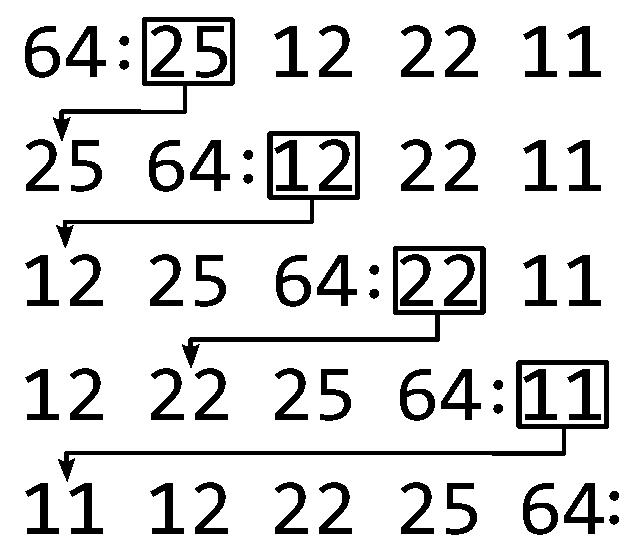
\includegraphics[height=45mm]{slike/insertionsort.pdf}
    \end{center}
    \vspace{-0.7cm}
    \caption[Urejanje z vstavljanjem]{Grafična predstavitev urejanja z navadnim
    vstavljanjem.}
    \caption*{{ \small Urejanje z vstavljanjem je prikazano 
    na petih naključno razporejenih številih.
    Urejeni del je od neurejenega ločen z dvopičjem, puščice nakazujejo mesto,
    na katerega smo vstavili trenutni element.}}
    \label{fig:insertionsortimage}
\end{figure}

Algoritem navadnega vstavljanja je v psevdokodi napisan kot algoritem~\ref{algo:insertionsort}.

\begin{algorithm}[h!t!]
  \caption{Urejanje z vstavljanjem}\label{algo:insertionsort}
  \begin{algorithmic}[1]
    \Function{insertionsort}{a, prvi, zadnji}
        \For{i}{prvi + 1}{zadnji}
            \State $x \gets a[i]$
            \State $j \gets i - 1$
            \While{$(x < a[j]) \wedge (j \geq 0)$} \label{line:insertionsortwhile} 
                \State $a[j+1] \gets a[j]$
                \State $j \gets j - 1$
            \EndWhile
            \State $a[j+1] \gets x$
        \EndFor
    \EndFunction
  \end{algorithmic}
\end{algorithm}

Med postopkom iskanja pravega mesta je dobro med izvajanji primerjanj 
sproti premikati elemente. Z drugimi besedami pustiti $x$, da se ``pogrezne'' tako, da $x$
primerjamo z naslednjim elementom $a_j$ in ga bodisi vstavimo, če je ključ $a_j$ manjši
ali enak $x$ ali pa $a_j$ premaknemo na desno ter nadaljujemo proti levi, če še nismo pri
levem robu polja. Postopek ``pogrezanja'' lahko ustavita ta dva ločena
pogoja, kot je prikazano v \emph{while} zanki v
algoritmu~\ref{algo:insertionsort} na vrstici~\ref{line:insertionsortwhile}.  Ko vstavimo še zadnji element v že 
urejeno zaporedje, smo z urejanjem zaključili.

\subsubsubsection{Časovna in prostorska zahtevnost} \nopagebreak
Časovna zahtevnost je v 
\begin{itemize}
  \item najboljšem primeru $\mathcal{O}(n)$
  \item povprečnem primeru $\mathcal{O}(n^2)$
  \item najslabšem primeru $\mathcal{O}(n^2)$
\end{itemize}

Prostorska zahtevnost je v vsakem primeru $\mathcal{O}(1)$, saj se vse premene dogajajo na
mestu.
(povz. po Wirth, 1985, str. 109.)

Spodnja časovna meja ustreza primeru, ko so elementi na začetku že urejeni, zgornja pa primeru,
ko so elementi na začetku nasprotno urejeni. Podani algoritem opisuje tudi stabilen postopek urejanja, kajti medsebojni
vrstni red elementov z enakimi ključi ostane nespremenjen.

Urejanje z navadnim vstavljanjem je zelo učinkovito na majhnih poljih. Učinkovito je tudi na že
skoraj urejenih poljih, saj se s tem približujemo obnašanju v najboljšem primeru.
Zaradi kvadratne časovne zahtevnosti je urejanje z navadnim vstavljanjem zelo neučinkovito na
dolgih poljih, če ta niso že skoraj urejena.

\subsubsection{Urejanje z izbiranjem}
\label{chapter:selectionsort}
Urejanje z izbiranjem (\emph{angl.} selection sort) je eden najenostavnejših primerjalnih sortirnih
algoritmov.

Algoritem je sledeč:\vspace{-1ex}
\begin{enumerate}\addtolength{\itemsep}{-0.65\baselineskip}
  \item najdi element z najmanjšim ključem
  \item zamenjaj ga s prvim elementom
  \item ponovi zgornja koraka za ostanek polja.
\end{enumerate}

Polje je med urejanjem razdeljeno na dva dela: podpolje že urejenih elementov, ki se
nahaja na začetku in podpolje elementov, ki jih je še potrebno urejati in zasedajo
preostali del polja. Postopek urejanja z izbiranjem je prikazan na
sliki~\ref{fig:selectionsortimage}. \\

\begin{figure}[ht]
    \begin{center}
        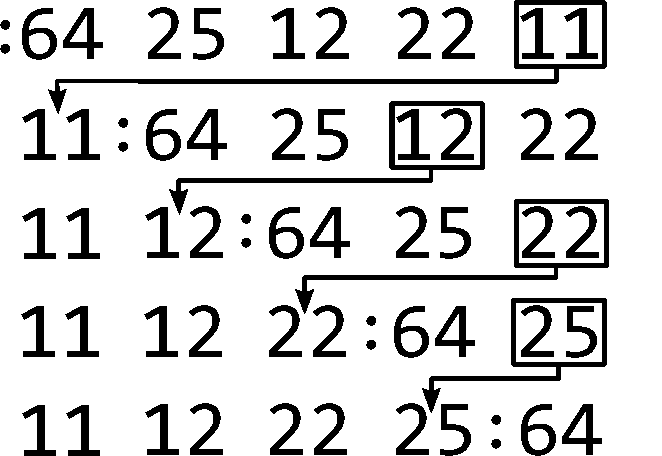
\includegraphics[height=40mm]{slike/selectionsort.pdf}
    \end{center}
    \vspace{-0.7cm}
    \caption[Urejanje z izbiranjem]{Grafična predstavitev urejanja z izbiranjem.}
    \caption*{{\small Najmanjši elementi v drugem delu polja so obkroženi, puščica ponazarja, kako jih
    vstavimo na konec prvega dela. Dela sta ločena z dvopičjem.}}
    \label{fig:selectionsortimage}
\end{figure}

V psevdokodi je urejanje z izbiranjem zapisano kot algoritem~\ref{algo:selectionsort}.

\begin{algorithm}[h!t!]
  \caption{Urejanje z izbiranjem}\label{algo:selectionsort}
  \begin{algorithmic}[1]
    \Function{selectionsort}{a, prvi, zadnji}
        \For{i}{prvi}{zadnji}
            \State $x \gets i$
            \For{j}{i + 1}{zadnji}
                \If{$a[j] < a[x]$}
                    \State $x \gets j$
                \EndIf
            \EndFor
            \Swap{a[x]}{a[i]}
        \EndFor
    \EndFunction
  \end{algorithmic}
\end{algorithm}

\subsubsubsection{Časovna in prostorska zahtevnost} \nopagebreak
Časovna zahtevnost je v vsakem primeru enaka in sicer $\mathcal{O}(n^2)$.

Prostorska zahtevnost je v najboljšem, povprečnem in najslabšem primeru $\mathcal{O}(1)$, 
saj algoritem opravlja vse premene na mestu.
(povz. po Wirth, 1985, str. 113.) 

Ker ima urejanje z izbiranjem v vsakem primeru kvadratno časovno zahtevnost, je neprimerno
za daljša polja. Urejanje z izbiranjem tudi ni odvisno od prvotnega vrstnega reda,
saj mora za iskanje najmanjšega elementa vedno pregledati celoten ostanek polja.
Njegova prednost je v tem, da stori zelo malo zamenjav elementov, kar je še posebej
primerno takrat, ko je premikanje elementov drago (imamo velike elemente).

\subsubsection{Hitro urejanje}
\label{chapter:quicksort}
Hitro urejanje ali urejanje s porazdelitvami\footnote{vir: IJS-jev slovar računalniških izrazov
\url{http://www.ijs.si/cgi-bin/rac-slovar}}(\emph{angl.} quicksort) je eden izmed
najučinkovitejših sortirnih algoritmov, ki jih poznamo, razvil pa ga je C. A. R. Hoare.
Je primerjalni sortirni algoritem, ki je zgrajen na principu deli in vladaj.

Sortiranje s porazdelitvami temelji na dejstvu, da moramo premene opravljati na večje
razdalje, da bi bile učinkovitejše. Recimo, da imamo $n$ nasprotno urejenih elementov.
V tem primeru jih lahko urejamo z le $^n/_2$ premenami tako, da najprej premenjamo prvega
in zadnjega in se postopoma pomikamo proti sredini. Seveda je to možno le, če vemo, da so 
elementi natanko nasprotno urejeni.

Prejšnji primer nas napelje na naslednji algoritem: 
izberemo poljuben element (recimo mu pivot in ga označimo z $x$), nato začnemo 
polje $a$ pregledovati z leve, dokler ne najdemo elementa $a_i > x$ in nato z desne dokler ne 
najdemo elementa $a_i < x$. Elementa sedaj medsebojno zamenjamo in nadaljujemo s 
pregledovanjem in premenami, dokler se ne srečamo nekje na sredi polja.
Polje je sedaj razdeljeno na levi del s ključi manjšimi od $x$ in na desni del
s ključi večjimi od $x$. Pivot nato umestimo med oba dela, kar je tudi njegovo končno
mesto, in metodo ponovimo na delih levo in desno od pivota, dokler ne pridemo do že urejenih
podpolj, torej tistih z dolžino manjšo ali enako 1. 

Iz prejšnjega algoritma ugotovimo, da je izbira pivota zelo
pomembna. Pogosto je, da za pivot vzamemo kar zadnji element, vendar to sproži ravno
najslabšo možnost izvajanja programa, če so elementi že urejeni. Zato sem v svoji
implementaciji za pivot vzel mediano prvega, srednjega in zadnjega elementa oziroma t.i.
mediano treh. Pogosta izbira je tudi naključni pivot. Postopek urejanja s
porazdelitvami je prikazan na sliki~\ref{fig:quicksortimage}.
V psevdokodi je algoritem hitrega urejanja zapisan kot algoritem~\ref{algo:quicksort}.

\begin{figure}[ht]
    \begin{center}
        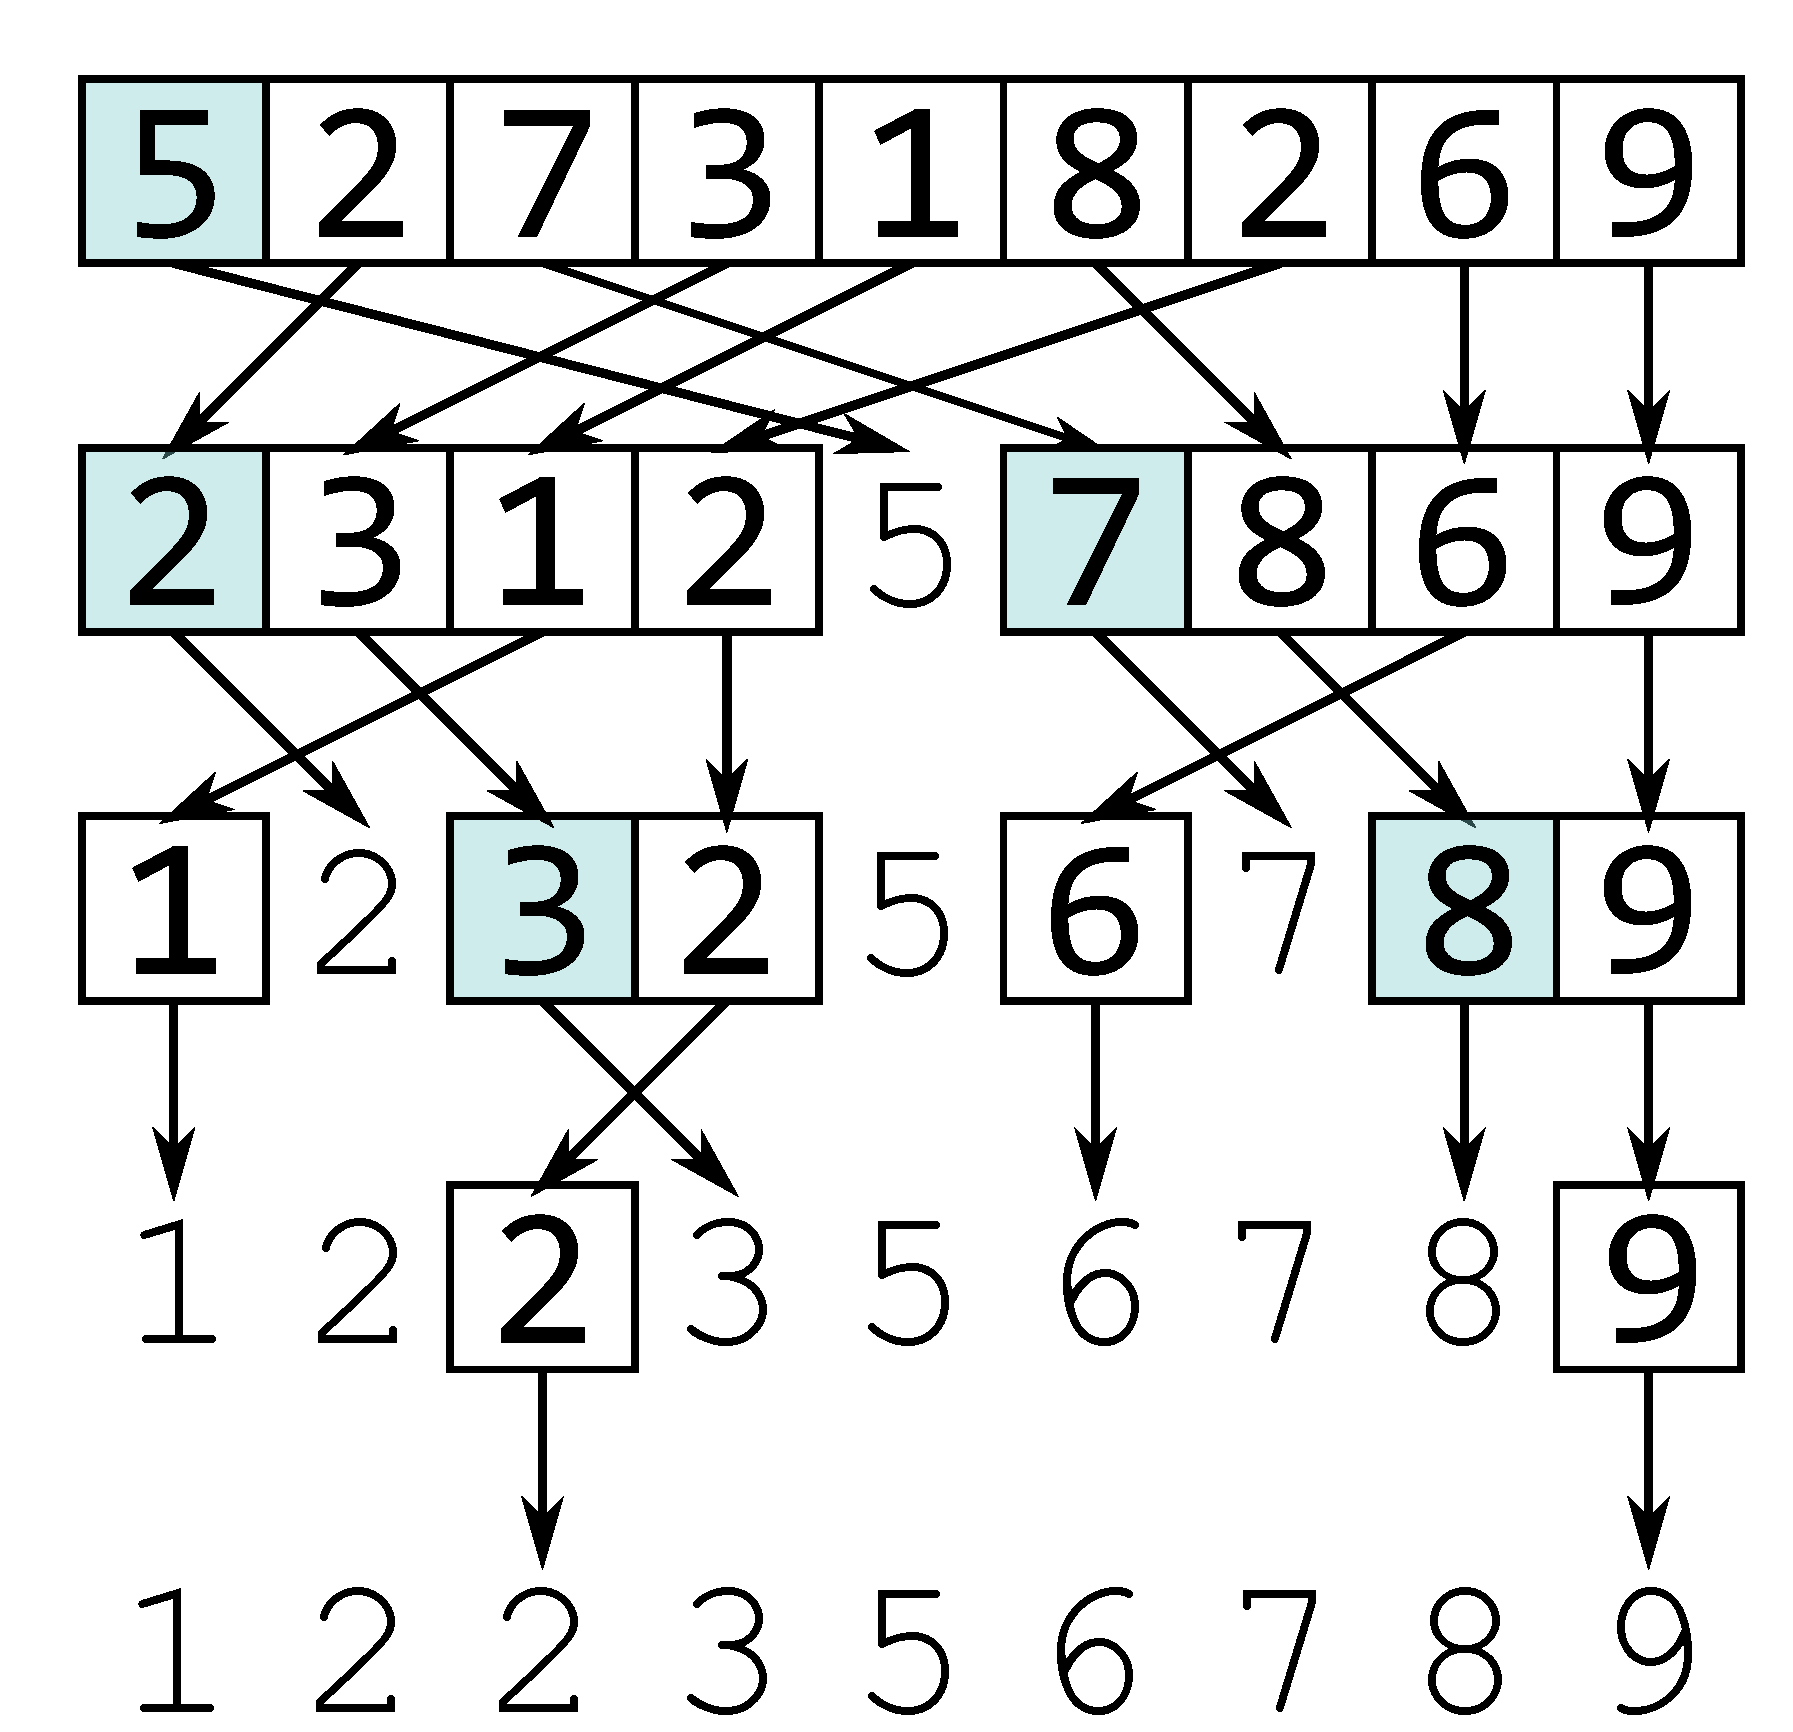
\includegraphics[height=50mm]{slike/quicksort.pdf}
    \end{center}
    \vspace{-0.6cm}
    \caption[Hitro urejanje]{Grafična predstavitev hitrega urejanja.}
    \caption*{{\small Hitro urejanje je prikazano na primeru devetih naključno razporejenih 
števil. Izbrani pivoti so obarvani. Vsaka vrstica predstavlja svojo globino rekurzije.}}
    \label{fig:quicksortimage}
\end{figure}

\begin{algorithm}[h!t!]
  \caption{Hitro urejanje}\label{algo:quicksort}
  \begin{algorithmic}[1]
    \Function{quicksort}{a, prvi, zadnji}
        \If{$zadnji - prvi < 2$} \Return \EndIf
        \State $s \gets prvi$
        \State $e \gets zadnji - 1$
        \State $m \gets \lfloor(s+e)/2\rfloor$
        \If{$(a[m] < a[s] < a[e]) \vee (a[e] < a[s] < a[m])$}
            \Swap{a[s]}{a[e]}
            \Comment{a[s] je mediana treh}
        \ElsIf{$(a[e] < a[m] < a[s]) \vee (a[s] < a[m] < a[e])$}
            \Swap{a[m]}{a[e]}
            \Comment{a[m] je mediana treh}
        \EndIf

        \State $pivot \gets a[e]$
        \State $e \gets e - 1$

        \While{$s \leq e$}
            \While{$(s \leq e) \wedge (a[s] < pivot)$}
                \Comment{prvi element z leve, večji od pivota}
                \State $s \gets s + 1$
            \EndWhile
            \While{$(s \leq e) \wedge (a[e] \geq pivot)$}
                \Comment{prvi z desne, ki je  manjši od pivota}
                \State $e \gets e - 1$
            \EndWhile
            \If{$s < e$}
                \Swap{a[s]}{a[e]}
            \EndIf
        \EndWhile
        \State $a[zadnji - 1] \gets a[s]$
        \State $a[s] \gets pivot$
        \State \textsc{quicksort}$(a, prvi, s)$
        \State \textsc{quicksort}$(a, s + 1, zadnji)$
    \EndFunction
  \end{algorithmic}
\end{algorithm}

\subsubsubsection{Časovna in prostorska zahtevnost}
Časovna zahtevnost je v
\begin{itemize}
  \item najboljšem primeru $\mathcal{O}(n\log_2 n)$
  \item povprečnem primeru $\mathcal{O}(n\log_2 n)$
  \item najslabšem primeru $\mathcal{O}(n^2)$
\end{itemize}

Prostorska zahtevnost je v najboljšem in povprečnem primeru $\mathcal{O}(\log_2 n)$, 
saj algoritem opravlja premene na mestu, vsak rekurziven klic pa zahteva $\mathcal{O}(1)$ prostora.
V najslabšem primeru je rekurzivnih klicev $n$, zato zahteva algoritem
$\mathcal{O}(n)$ prostora.
(povz. po Wirth, 1985, str. 128.)

Hitro urejanje je eden najhitrejših sortirnih algoritmov, kar jih
poznamo. Svojo hitrost dolguje arhitekturi današnjih procesorjev, ki imajo
malo registrov in precej notranjega pomnilnika, saj lahko pivot ponavadi shranimo v
register, kar prihrani veliko poizvedb do pomnilnika. Dober je na enakomerno
porazdeljenih podatkih, a kljub pazljivemu izbiranju pivotov obstaja možnost neželenega
najslabšega primera, čeprav je zelo neverjetna. Znana izboljšava hitrega
urejanja je tudi, da krajših polja ne uredimo spet z hitrim urejanjem temveč s
kakšnim hitrejšim algoritmom za kratka polja, na primer z urejanjem z
vstavljanjem.

\subsubsection{Urejanje s kopico}
\label{chapter:heapsort}
Urejanje s kopico (\emph{angl.} heapsort) je sortirni algoritem,
ki si pri urejanju pomaga s kopico.

Maksimalna kopica je dvojiško drevo, pri katerem velja, da je ključ očeta
vedno večji od ključa otroka. Privzemimo, da je levo poravnano.
Maksimalno kopico lahko predstavimo v polju, kjer je koren kopice na mestu 
1, in velja, da sta otroka elementa na mestu $i$ na mestih $2i$ in $2i + 1$.
Maksimalno kopico, prikazano na sliki~\ref{fig:kopica}, tako predstavimo kot tako zaporedje elementov $a_i, a_{i+1}, \ldots,
a_n$, da za njih velja:
\begin{align*}
  a_i &\geq a_{2i} \\
  a_i &\geq a_{2i+1}
\end{align*}
pri vseh $i = 1 \ldots \lfloor ^n/_2 \rfloor$.
(povz. po Kozak, 1986, str. 104.)

\begin{figure}[ht]
    \begin{center}
        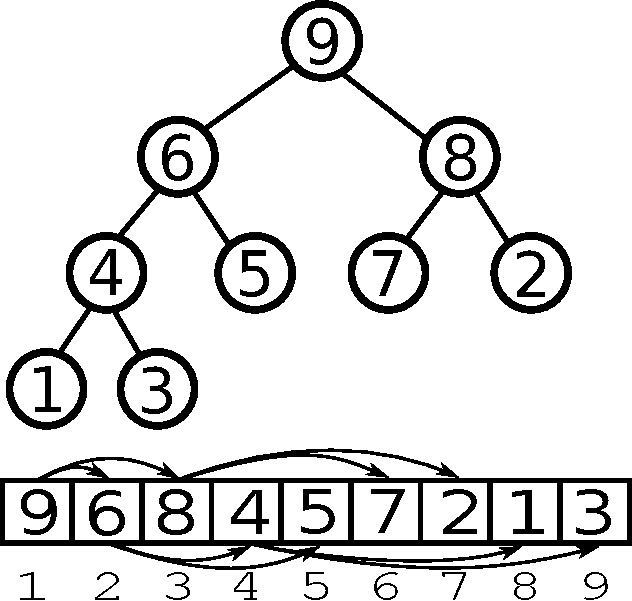
\includegraphics[height=45mm]{slike/heap.pdf}
    \end{center}
    \vspace{-0.7cm}
    \caption[Kopica]{Kopica.}
    \caption*{{\small Predstavitev maksimalne kopice kot dvojiškega
    drevesa (zgoraj) in predstavitev maksimalne kopice v polju (spodaj). Vidimo,
    da je invarianta kopice vzpostavljena v obeh primerih. Pri predstavitvi
    kopice v polju so pod poljem prikazani tudi indeksi posameznih elementov.}}
    \label{fig:kopica}
\end{figure}


Urejanje s kopico podatke najprej preuredi v maksimalno kopico. To naredimo tako,
da za vse elemente, ki imajo otroke, ponovimo naslednji postopek:
Če je katerih izmed otrok večji od očeta, potem očeta zamenjamo z večjim izmed
obeh otrok, ter ponovimo postopek dokler ni zadoščeno invarianti kopice.
Nato odstranimo koren kopice -- največji element -- in ga zamenjamo z zadnjim
elementom kopice. Potem ponovno vzpostavimo invarianto kopice na preostanku
elementov in zopet odstranimo korenski element ter ga
zamenjamo s tistim na predzadnjem mestu. To ponavljamo, dokler ni kopica dolga le en
element. Urejanje s kopico je prikazano na sliki~\ref{fig:heapsortimage}.
V psevdokodi je algoritem urejanja s kopico prikazan kot
algoritem~\ref{algo:heapsort}. \\

\begin{figure}[ht]
    \begin{center}
        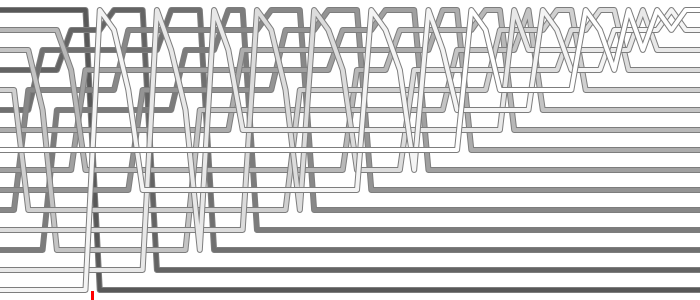
\includegraphics[height=45mm]{slike/Heap.png}
    \end{center}
    \vspace{-0.7cm}
    \caption[Urejanje s kopico]{Grafična predstavitev urejanja s kopico.}
    \caption*{{\small Vsaka črta predstavlja svoj element; temnejša kot je črta,
    večji je element. Do pike na dnu slike poteka urejanje podatkov v kopico, 
    nato pa odstranjevanje največjega elementa in ponovna vzpostavitev kopice 
    vse do konca. Slika je bila ustvarjena s programsko kodo, dostopno na spletnem
    naslovu: \url{http://corte.si/posts/code/visualisingsorting/index.html.}}}
    \label{fig:heapsortimage}
\end{figure}

\begin{algorithm}[h!t!]
  \caption{Urejanje s kopico}\label{algo:heapsort}
  \begin{algorithmic}[1]
    \Function{heapsort}{a, prvi, zadnji}
        \State \textsc{nakopiči}$(a, prvi, zadnji)$
        \While{$prvi < zadnji$}
            \Swap{a[prvi]}{a[zadnji]};
            \State $zadnji \gets zadnji - 1$
            \State \textsc{pogrezni}$(a, prvi, prvi, zadnji)$
        \EndWhile
    \EndFunction
    \\
    \Function{nakopiči}{a, prvi, zadnji}
        \State $zacetek \gets \lfloor(prvi + zadnji) / 2\rfloor - 1$
        \While{$zacetek \geq prvi$} \Comment{pogreznemo vse elemente, ki imajo otroke}
            \State $odmik \gets koren - prvi$
            \State \textsc{pogrezni}$(a, prvi, zacetek, zadnji)$
            \State $zadnji \gets zadnji - 1$
        \EndWhile
    \EndFunction
    \\
    \Function{pogrezni}{a, prvi, koren, zadnji}
        \State $odmik \gets koren - prvi$
        \While{$koren + odmik < zadnji$} \Comment{dokler ima koren vsaj enega otroka}
            \State $otrok \gets koren + odmik + 1$
            \State $zamenjava \gets koren$ \Comment{zapomnimo si, s čim naj zamenjamo koren}
            \If{$a[koren] < a[otrok]$} \Comment{če je otrok večji od korena}
            \State $zamenjava = otrok$\Comment{potem moramo zamenjati prvega otroka}
            \EndIf \Comment{če drugi otrok obstaja in je večji od trenutne zamenjave}
            \If{$(otrok + 1) \leq (zadnji \wedge zamenjava < a[otrok + 1])$}
                \State $zamenjava = otrok + 1$\Comment{potem zamenjamo njega}
            \EndIf
            \If{$zamenjava \neq koren$}
                \Swap{a[zam]}{a[koren]}
                \State $koren \gets zamenjava$
                \State $odmik \gets koren - prvi$
            \Else
                \State \Return 
            \EndIf
        \EndWhile
    \EndFunction
  \end{algorithmic}
\end{algorithm}

\subsubsubsection{Časovna in prostorska zahtevnost}
Časovna zahtevnost je v najboljšem, povprečnem in najslabšem primeru $\mathcal{O}(n\log_2 n)$.

Prostorska zahtevnost je v vsakem primeru $\mathcal{O}(1)$, saj je kopica predstavljena kar v
polju, ki ga urejamo, in ker se vse premene dogajajo na mestu.
(povz. po Wirth, 1985, str. 123.)

Čas izvajanja urejanja s kopico je neodvisen od morebitne urejenosti podatkov v polju,
kot lahko razberemo iz časovne zahtevnosti. Zaradi dokaj zapletenega postopka urejanja
na manjših poljih ni tako hiter, je pa čedalje hitrejši, ko se dolžina polja
povečuje.

\subsubsection{Urejanje z zlivanjem}
\label{chapter:mergesort}
Urejanje z zlivanjem (\emph{angl.} merge sort) je primerjalni sortirni algoritem, 
zgrajen na principu deli in vladaj. Razvil ga je John von Neumann leta 1945.
Urejanje z zlivanjem uporablja idejo, da je v urejeno polje hitreje združiti dve že
urejeni polji, kot pa dve še ne urejeni. 
Algoritem urejanja z zlivanjem ureja tako:
\begin{enumerate}
  \item če je polje dolgo 0 ali 1, je že urejeno, če ne:
  \item razdeli polje v dve približno enako dolgi podpolji
  \item urejaj podpolji 
  \item združi podpolji nazaj v celotno urejeno polje.
\end{enumerate}
Algoritem je grafično prikazan na sliki~\ref{fig:mergesortimage} na primeru sedmih
naključno izbranih števil.
V psevdokodi je urejanje z zlivanjem zapisano kot algoritem~\ref{algo:mergesort}. 

\begin{figure}[ht]
    \begin{center}
        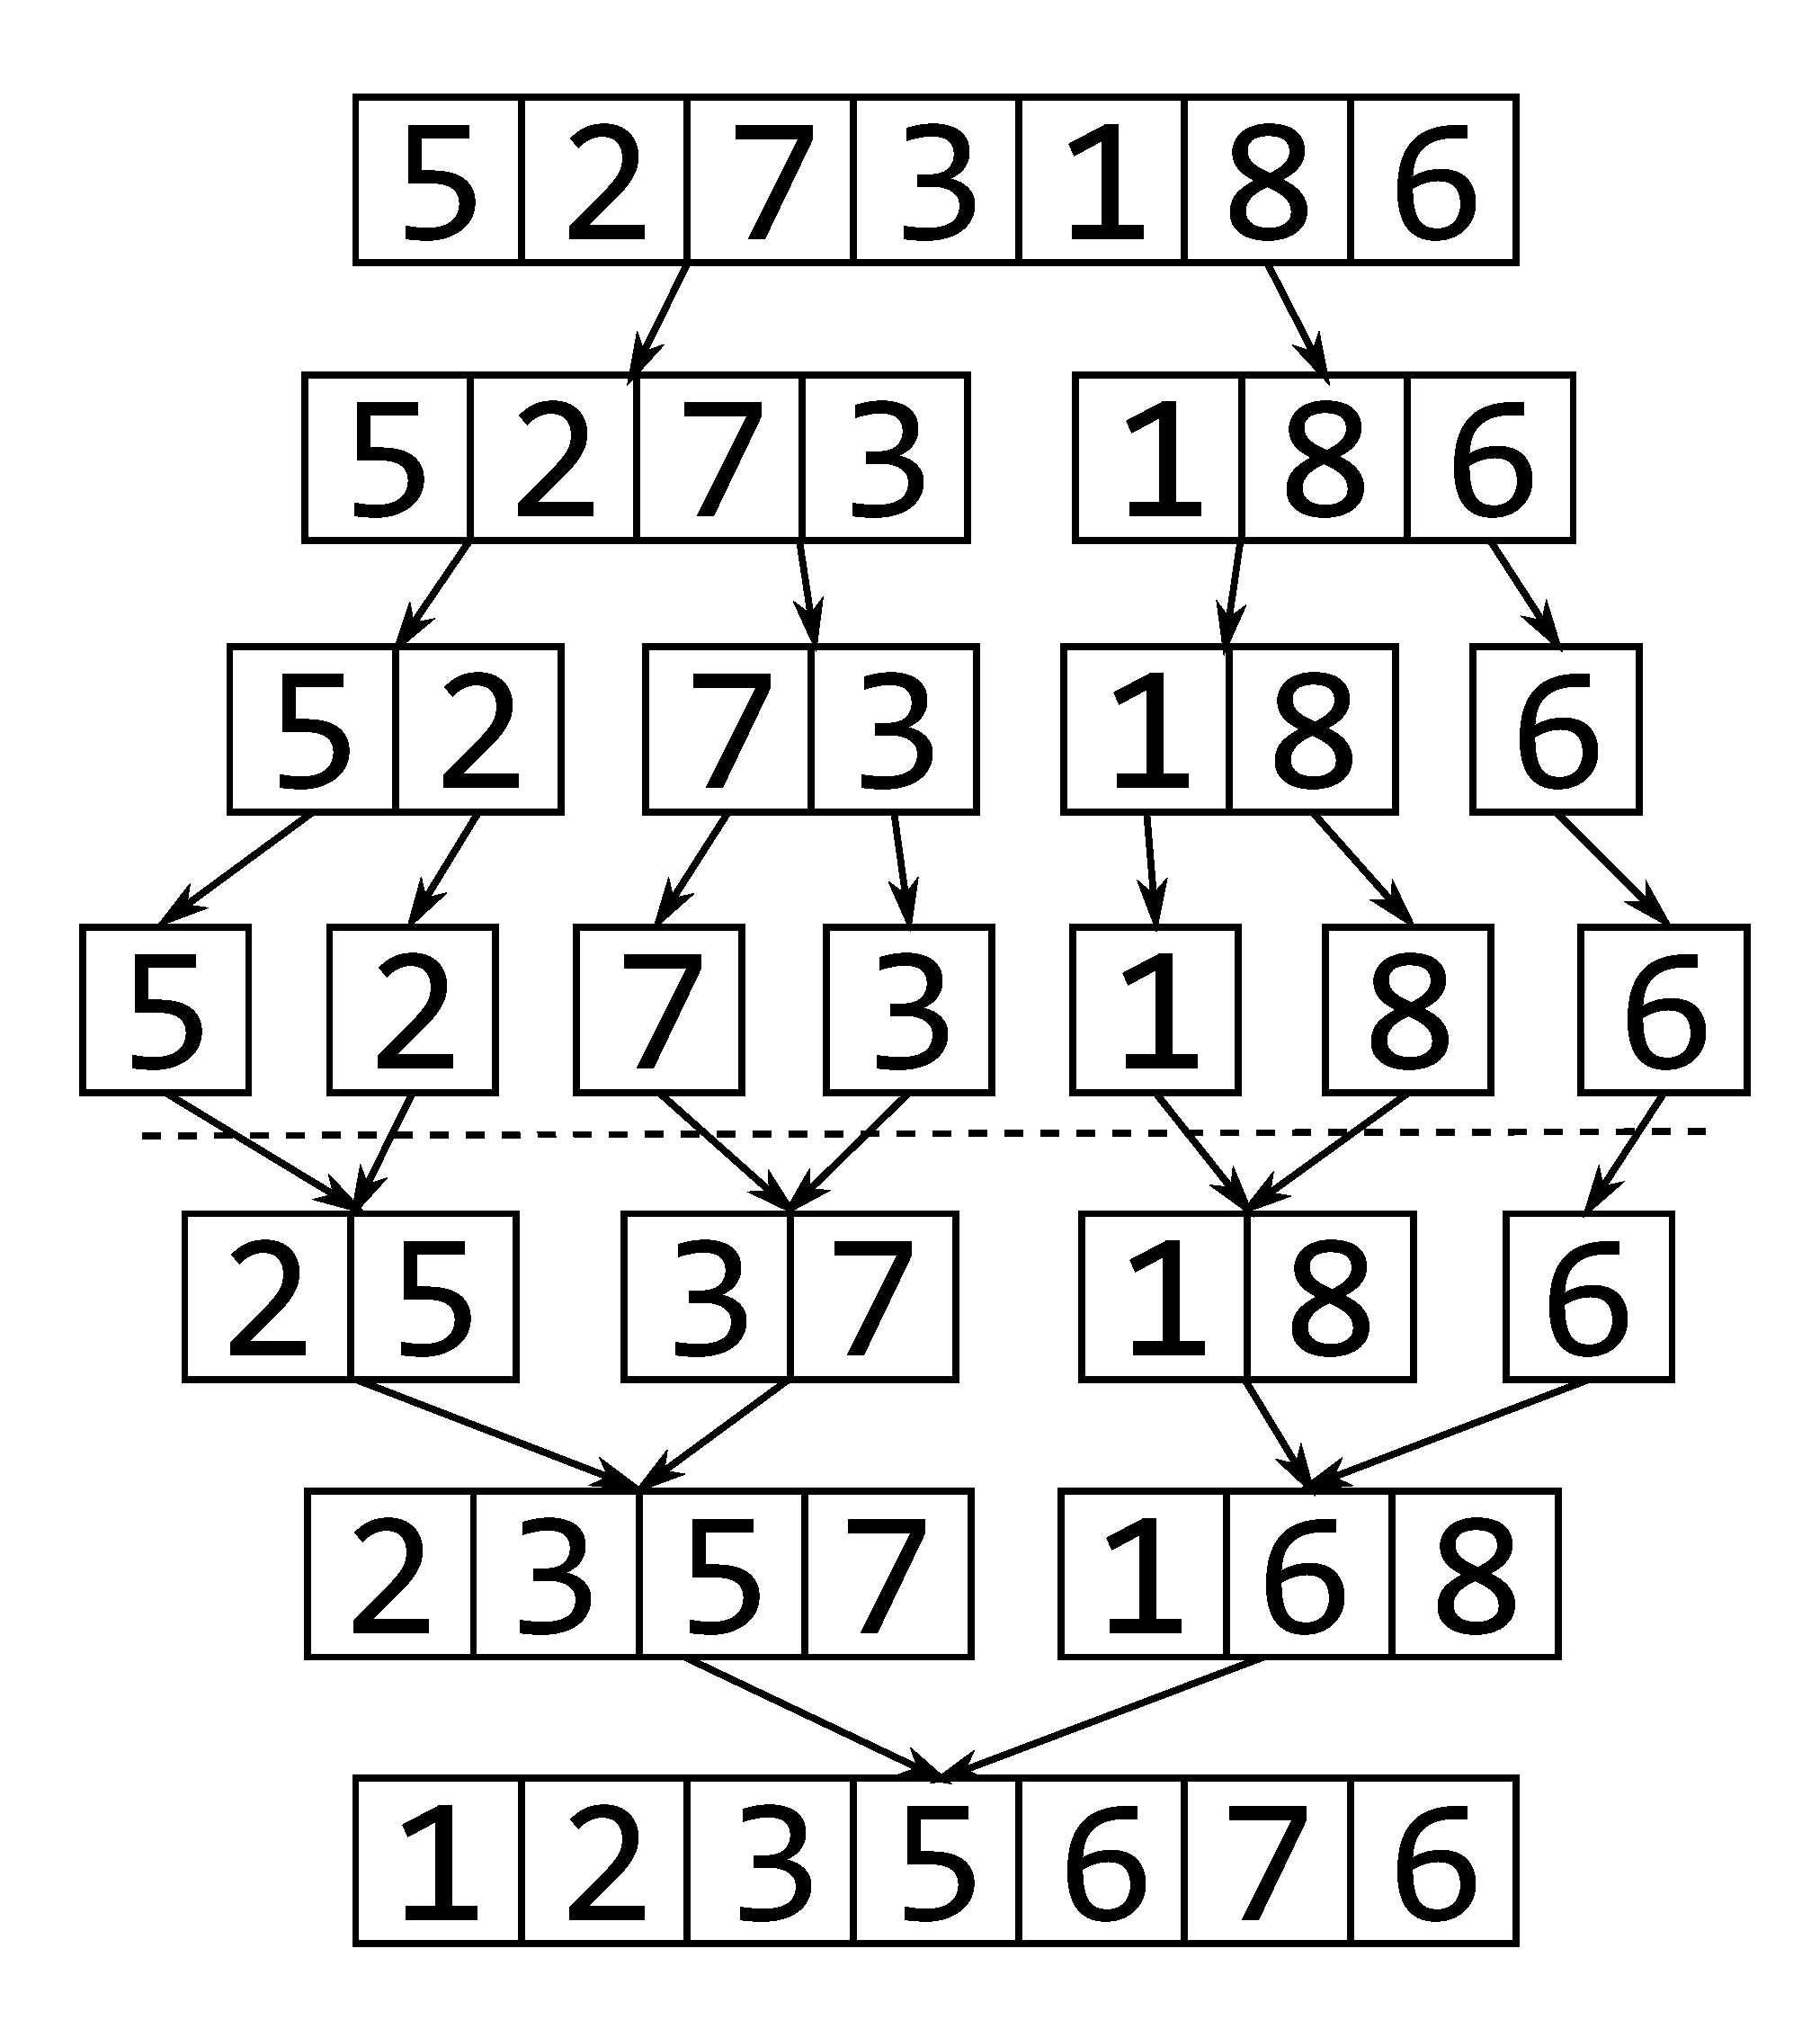
\includegraphics[height=60mm]{slike/mergesort.pdf}
    \end{center}
    \vspace{-0.7cm}
    \caption[Urejanje z zlivanjem]{Grafična predstavitev urejanja z zlivanjem.}
    \caption*{{\small Vsaka vrstica števil predstavlja svojo 
    globino rekurzije, vse dokler niso polja dolga le po en element.
    Nato se začne izvajati četrta točka algoritma, ponazorjena z vrsticami
    nižje od črtkane črte, ki združi podpolja v urejeno polje.}}
    \label{fig:mergesortimage}
\end{figure}

\begin{algorithm}[h!t!]
  \caption{Urejanje z zlivanjem}\label{algo:mergesort}
  \begin{algorithmic}[1]
    \Function{mergesort}{a, prvi, zadnji}
        \If{$zadnji - prvi < 2$} \Return \EndIf
        \State $srednji \gets \lfloor(prvi + zadnji) / 2\rfloor$
        \State \textsc{mergesort}$(a, prvi, srednji)$
        \State \textsc{mergesort}$(a, srednji + 1, zadnji)$
        \State \textsc{merge}$(a, prvi, srednji, zadnji)$
    \EndFunction
    \\
    \Function{merge}{a, prvi, srednji, zadnji}
        \State $i \gets prvi$
        \State $j \gets srednji$
        \State $t \gets prvi$
        \State $za\check{c}asen \gets$\textsc{kopiraj}$(a, prvi, zadnji)$ 
        \Comment{kopiramo polje $a$ v pomnilnik}
        \While{$i < srednji \wedge j < zadnji$}
            \If{$a[i] < a[j]$}
                \State $a[t] \gets za\check{c}asen[i]$
                \State $i \gets i + 1$
            \Else
                \State $a[t] \gets za\check{c}asen[j]$
                \State $j \gets j + 1$
            \EndIf
            \State $t \gets t + 1$
        \EndWhile
        \While{$i < srednji$}
            \State $a[t] \gets za\check{c}asen[i]$
            \State $t \gets t + 1$
        \EndWhile
        \While{$j < srednji$}
            \State $a[t] \gets za\check{c}asen[j]$
            \State $t \gets t + 1$
        \EndWhile
    \EndFunction
  \end{algorithmic}
\end{algorithm}

\subsubsubsection{Časovna in prostorska zahtevnost} \nopagebreak
Časovna zahtevnost je v najboljšem, povprečnem in najslabšem primeru 
$\mathcal{O}(n\log_2 n)$. Časovna zahtevnost urejanja z zlivanjem ni odvisna od
morebitne že delne urejenosti ali neurejenosti podatkov v polju. 

Prostorska zahtevnost je v vsakem primeru $\mathcal{O}(n)$.\\ % ker O(n + log n)
(povz. po Knuth, 1998, str. 158.) \\

V praksi je urejanje z zlivanjem najbolj učinkovito na
sekvenčnih medijih, kot na primer tračnih enotah, ali na podatkovnih strukturah, ki nimajo hitrega
neposrednega dostopa do nekega elementa z njegovim indeksom, kot na primer povezani seznami.

\subsection{Opredelitev problema in cilji}
Problem naloge je poiskati najučinkovitejši sortirni algoritem. Tak algoritem
mora biti prilagodljiv, saj mora biti čim hitrejši na različnih računalnikih in
različnih tipih podatkov. Prav to je problem sortirnih algoritmov, ki so
trenutno dostopni v vgrajenih knjižnicah za urejanje, kot na primer
\emph{algorithm} v C++. Algoritmi implementirani v knjižnicah so zelo
optimizirani za že vgrajene tipe in so napisani tako, da so hitri na večini
računalnikov. To pomeni, da vgrajeni algoritem odlično ureja vgrajene tipe na
povprečnem računalniku, ko pa se oddaljujemo od povprečja ali pa algoritmu damo
za urejati netipične podatke, se algoritem oddalji od optimalnosti. V tej nalogi
želimo poiskati tak sortirni algoritem, ki se lahko prilagaja računalniku in
podatkom, ter eksperimentalno ugotovi, kaj je pri trenutnih pogojih optimalen
sortirni algoritem. Zaželeno je tudi, da je enostaven za uporabo, vendar ima uporabnik
kljub temu nad njim dovolj nadzora.

\subsection{Hipoteze}
\begin{enumerate}
  \item \label{hip:dif:type:dif:algo} Učinkovitost sortirnega
    algoritma je zelo odvisna od lastnosti elementov, ki jih urejamo.
  \item \label{hip:komp:vs:nekomp} Kompoziten sortirni algoritem se obnese boljše na različnih tipih podatkov kot vsak
    posamezen algoritem.
    % kaj pa kakšna da bo beatov build-in sort
\end{enumerate}

\pagebreak
\mbox{}

\pagebreak

\section{Metode dela}
Za preverjanje hipotez sem si izbral eksperiment. Hipotezi je z njim najlažje
potrditi ali ovreči, drugih virov na to temo pa ni v izobilju. Pri pripravi eksperimenta
sem potreboval tudi nekaj sekundarnih virov. Za izvedbo eksperimenta sem implementiral vse 
v teoretičnem delu opisane sortirne algoritme. Za implementacijo sem si izbral programski 
jezik C++, predvsem zato, ker se program prevede v strojno kodo, nad katero ima programer
veliko nadzora. Zmožen je optimizacije na najnižji ravni, medtem ko je pisanje kode kljub
temu nezahtevno opravilo, kot pri drugih programskih jezikih tretje generacije.

\subsection{Implementacija sortirnih algoritmov}
\label{chapter:sortimplementation}
Vsak izmed sortirnih algoritmov je implementiran kot funkcija z dvema parametroma.
Vsaka funkcija sprejme dva iteratorja z naključnim dostopom (\emph{Random Access
Iterator} ali kar \emph{RAI}),
ki kažeta na prvi element dela polja, ki ga urejamo, in na prvi element za koncem tega dela.
Slednji je lahko neveljaven v polju (kaže preko njegovega konca).
Tako obliko funkcij sem si izbral predvsem zato, ker je v skladu z zapisom, ki ga uporablja
\mbox{C++-ova} knjižnica \emph{algorithm}. Drugi razlog je, da s tem zapisom dosežemo minimalno število
parametrov pri želeni funkcionalnosti. Če bi želeli le en parameter, bi bilo to
izvedljivo, vendar bi se morali odpovedati zmožnosti, da lahko sedaj uredimo le željeni
del polja. V primeru zgolj enega parametra to ne bi bilo možno, vedno bi se
urejalo celotno polje.

Vsak sortirni algoritem, ki sem ga implementiral, ureja zgolj z uporabo operatorja $<$
(``je manjše''), ki je usklajen z relacijo linearne urejenosti $\leq$ iz uvoda. Vsak
algoritem je definiran kot funkcija tipa \emph{void}, kar pomeni, da ne vrne ničesar, in
torej spremeni vrstni red elementov polja, ki ji ga podamo.

\subsection{Implementacija kompozitnega sortirnega algoritma}
\label{chapter:tweaksort}
Ker so sortirni algoritmi vsak zase dobri na zgolj nekaterih dolžinah polj in se pri tej
lastnosti razlikujejo, nas to privede do zamisli, da bi pri dani dolžini $n$ uporabili tisti
sortirni algoritem, ki je pri tem $n$ najboljši. Ta zamisel je prikazana na sliki~\ref{fig:tweaksortidea}.
Torej moramo vedeti, pri katerem $n$ je
potrebno uporabiti kateri sortirni algoritem, kar pa si bomo morali zapomniti
v konfiguracijo.% V ta
%namen sem definiral tip \emph{conf\_\!t}, v katerem je shranjena konfiguracija kompozitnega
%sortirnega algoritma. 

\begin{figure}[ht]
    \begin{center}
        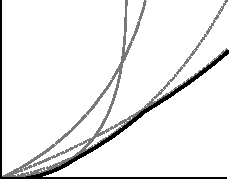
\includegraphics[width=80mm,height=45mm]{slike/tweaksortidea.pdf}
    \end{center}
    \vspace{-0.7cm}
    \caption[Ideja kompozitnega sortirnega algoritma]{Ideja kompozitnega sortirnega algoritma.}
    \caption*{{\small Sive krivulje prikazujejo algoritme, ki niso kompozitni, črna pa kompozitni algoritem.
    Krivulja kompozitnega algoritma ustreza spodnji meji ostalih krivulj, torej se vedno uporablja 
    najhitrejši sortirni algoritem pri tistem $n$.}}
    \label{fig:tweaksortidea}
\end{figure}

Konfiguracija pove, kateri sortirni algoritem naj se uporablja pri
katerem $n$. Lahko se jo predstavi kot niz znakov z zelo preprostimi
pravili. To je zaželeno predvsem zato, ker je konfiguracija namenjena temu, da je trajna
in berljiva ter da si jo uporabnik shrani. Ker je predstavljena kot niz
znakov, jo lahko tudi zapiše v datoteko in jo po želji tudi spremeni.

Kompozitni sortirni algoritem torej vedno uporabi tisti sortirni algoritem, ki je za  
trenutni $n$ določen v konfiguraciji. Tako spremenjen algoritem za urejanje bi v idealnem
primeru torej vhodno polje vedno uredil s čimbolj optimalnim sortirnim algoritmom.
Pomaga nam tudi dejstvo, da imajo nekateri algoritmi za urejanje zaradi principa deli in vladaj
še to lepo lastnost, da polja delijo na manjša podpolja. Ta manjša polja lahko spet
uredimo z optimalnih algoritmom za njihovo dolžino. To nam prinese možnost veliko hitrejšega
urejanja polj, saj se lahko odločimo, kateri sortirni algoritem bomo
uporabili, ne le za vhodno polje, temveč tudi za nekatera podpolja, ki jih ustvarijo
sortirni algoritmi, kot na primer hitro urejanje ali urejanje z zlivanjem.

Kompozitni sortirni algoritem mora torej pri svoji implementaciji poleg dveh 
iteratorjev z naključnim dostopom sprejeti tudi konfiguracijo. Procedura \emph{sort},
ki predstavlja kompozitni sortirni algoritem, deluje enako kot algoritem
\ref{algo:tweaksort}. 

\begin{algorithm}[h!t!]
  \caption{Kompozitni sortirni algoritem}\label{algo:tweaksort}
  \begin{algorithmic}[1]
    \Function{sort}{prvi, zadnji, conf}
        \State $n \gets zadnji - prvi$
        \State $algoritem \gets$ \textsc{najdi\_pravi\_algoritem}$(n, $\emph{conf}$)$
        \State \label{line:usealgo}Sortiraj z $algoritmom$.
    \EndFunction
  \end{algorithmic}
\end{algorithm}

Če v $algoritmu$, ki ga kličemo pri algoritmu~\ref{algo:tweaksort} na
vrstici~\ref{line:usealgo}, pride do rekurzivnega klica, naj kliče funkcijo \emph{sort} namesto
samega sebe.

V skladu s tem je bilo treba popraviti ostale sortirne algoritme, da namesto rekurzivnega
klica samega sebe kličejo proceduro \emph{sort} in tako pustijo, da se manjša polja morda uredijo z
drugim sortirnim algoritmom ter tako prispevajo k bolj učinkovitemu urejanju celotnega polja. Da pa
sortirni algoritmi sploh lahko kličejo glavno proceduro \emph{sort}, morajo kot
parameter prejeti tudi konfiguracijo, ki jo na koncu podajo nazaj proceduri \emph{sort}.

Funkcija \textsc{najdi\_pravi\_algoritem}, ki jo kliče procedura \textsc{sort}, se mora ob vsakem klicu odločiti, kateri
algoritem naj uporabi. Po celi konfiguraciji mora torej poiskati, kateri sortirni algoritem
naj uporabi, kar običajno terja časovno zahtevnost
$\mathcal{O}(n)$, kjer je $n$ število vnosov v konfiguracijo. Ker pa mora biti podana konfiguracija
smiselna, mora biti urejena naraščajoče. Torej lahko želeni dolžini priredimo sortirni
algoritem v logaritemskem času, in ne v linearnem, z dvojiškim iskanjem po urejenem polju, 
kot opisano v (Knuth, 1998, str. 409.). To je velika izboljšava še posebej za dolge konfiguracije, čeprav je lahko
pri krajših dvojiško iskanje celo malo počasnejše od linearnega.

\pagebreak
Da je konfiguracija smiselna, mora biti sestavljena iz zaporedij oblike
\[ :sort\ \konfarrow\ \check{s}tevilo; \edot\]
\begin{description}
  \item[$sort$] pove, kateri sortirni algoritem naj se uporablja na katerih poljih. Črka, ki
    prestavlja posamezen algoritem, je prva črka njegovega angleškega imena.
%    ($\mbox{$i - $\text{insertion}},\, s - \text{selection},\, q - \text{quick},\, h
%    - \text{heap},\, m - \text{merge}$)
  \item[$\check{s}tevilo$] predstavlja katerokoli možno dolžino polja, ki ga urejamo. Torej je lahko
    katerokoli nenegativno število. Dovoljeno je tudi število $-1$, ki predstavlja neskončno
($\infty$).
\end{description}

Zadostiti mora tudi naslednjima pogojema:
\begin{enumerate}
  \item števila morajo biti urejena naraščajoče in
  \item zadnje in samo zadnje število mora biti $-1$.
\end{enumerate}
S tema dvema pogojema dosežemo, da se za vse možne dolžine polj enolično
določi, kateri ``sort'' naj se uporablja, kar je tudi namen konfiguracije.

V nadaljevanju naloge bom pri vseh primerih konfiguracij zaradi večje preglednosti 
namesto ``\konfarrow'' pisal ``\lra''. \\

Primer smiselne konfiguracije:
\[ :i \lra 20;:h \lra 45;:i \lra 123;:q \lra 7925;:m \lra -1; \]
Konfiguracija upošteva vsa slovnična pravila.
Števila so urejena naraščajoče in samo zadnje število je $-1$. Ta konfiguracija je torej
pravilna in smiselna. Konfiguracija pove, da naj se polja, katerih dolžine so iz intervala $\left[0,
20\right]$ ureja z vstavljanjem, polja z dolžinami iz intervala $\left(20, 45\right]$ naj
se ureja s kopico, polja, ki imajo dolžine na intervalu $\left(45, 123\right]$ zopet z vstavljanjem,
polja z dolžinami na intervalu $\left(123, 7925\right]$ s porazdelitvami, polja, katerih dolžine pa so iz
intervala $\left(7925, \infty\right)$ oziroma tista, katerih dolžine so večje od 7925,
pa naj se ureja z zlivanjem. Tako je za prav vse možne dolžine enolično določeno, kateri
sortirni algoritem naj bo uporabljen.

Oglejmo si še nekaj realnih primerov, dobljenih za različne tipe podatkov.
\[ :i \lra 142;:q \lra -1;\]
\[ :m \lra -1; \]
Tudi ta dva primera sta smiselna. V prvem vidimo, da naj se uporablja urejanje z
vstavljanjem, če je dolžina polja manjša ali enaka 142, sicer naj se uporablja hitro
urejanje. Pri drugem primeru, ki je tudi eden izmed najkrajših možnih primerov
konfiguracije, se uporablja samo urejanje z zlivanjem.\\

%Primer nesmiselne konfiguracije:
%\[ :i \lra 60;:h \lra 45;:i \lra 145;:q \lra 7925;:m \lra 33456;:q \lra -1 \]
%Konfiguracija sicer upošteva vsa slovnična pravila, vendar je nesmiselna. Prva napaka je,
%da števila niso urejena naraščajoče, kar ne zagotavlja da je uporabljeni algoritem
%enolično določen. V konfiguraciji namreč piše, da naj se polja z
%dolžinami od 0 do 60 urejajo z vstavljanjem, tista z dolžinami od 60 do 45 pa s kopico.
%S tem sortirni algoritem za npr. polja dolžine 52 ni enolično določen.

%Še nekaj primerov nesmiselnih konfiguracij:
%\[ 50 \lra i:;q \lra -1; \]
%\[ :i \lra 22;:q \lra 450; \]
%\[ :s \lra 234;:q \lra -1;: m \lra 3456; \]
%Pri prvem primeru je konfiguracija ne le nesmiselna, temveč tudi nepravilno oblikovana.
%Pri drugem primeru je nesmiselno to, da konfiguracija ne vsebuje števila $-1$, in tako ne
%definira, kateri algoritem naj se uporablja za polja z dolžinami večjimi od 450.
%Pri zadnjem je nesmiselno to, da število $-1$ ni na koncu, torej so
%vsi vnosi za tem nepotrebni.

Definirajmo še množico \textbf{osnovnih konfiguracij}. To je množica konfiguracij, pri katerih
sortirni algoritem ni kompoziten, torej 
\[ \{``:i \lra -1;", ``:s \lra -1;", 
``:q \lra -1;", ``:h \lra -1", ``:m \lra -1;"\}. \]

\pagebreak
Ker se procedura \emph{sort} uporablja kot knjižnica, potebujemo tudi pretvornik
konfiguracije v niz znakov in obratno, zaradi česar je potrebno formalno definirati slovnico
konfiguracije, ki je (v notaciji BNF)\footnote{
Backus--Naur Form, standardna notacija za kontekstno-neodvisne slovnice.\\
vir: \url{http://www.cui.unige.ch/db-research/Enseignement/analyseinfo/AboutBNF.html}} 
sledeča:
\\
\begin{BNF}
  \begin{align*}
    \abnf{sort}{\q{i} \ali \q{s} \ali \q{q} \ali \q{h} \ali \q{m}}\\
    \abnf{število}{\in \N \ali \q{-1}} \\
    \abnf{vnos}{\q{:}\ntm{sort}\q{\mbox{--}\ \mbox{--}\ \mbox{$>$}}\ntm{število}\q{;}}\\
    \abnf{konfiguracija}{\ntm{vnos} | \ntm{konfiguracija}\ntm{vnos}}
  \end{align*}
\end{BNF}

\subsection{Iskanje optimalne konfiguracije}
\label{chapter:optimalconf}
Za hitrost procedure \emph{sort} je bistvena konfiguracija,
zato je iskanje optimalnega kompozitnega sortirnega algoritma pravzaprav iskanje optimalne
konfiguracije zanj. Ta razdelek je namenjen prav temu.  

Glavna ideja je, da dva kompozitna sortirna algoritma lahko primerjamo po času 
izvajanja. Tisti, ki porabi manj časa, je boljši pri dolžini polja, ki sta
ga urejala. S tem smo za algoritma $a$ in $b$ definirali relacijo $a$ je $n$-boljši od $b$:
\[ a \leq_n b \overset{\text{def}}{\Longleftrightarrow} a\ \text{je v povprečju na poljih dolžine $n$ boljši
od}\ b.\]
Tako lahko problem rešimo kar s požrešno metodo: 
pri posamezni dolžini ugotovimo, kateri algoritem je najboljši, in to vnesemo
v konfiguracijo. Glavni podatek, ki nam ga poda uporabnik, je meja učenja $M$. To je
največja dolžina, za katero bo algoritem še iskal optimalno konfiguracijo. Od te dolžine naprej
konfiguracija ni več nujno optimalna. Seveda v konfiguracijo pišemo le, če pride do 
spremembe na vodilnem mestu. Algoritem za iskanje najboljše konfiguracije je zapisan v
psevdokodi kot algoritem~\ref{algo:conf}.

Optimalno konfiguracijo bomo iskali takole: \\
za vsak $n$ od začetnega do $M$:
\begin{enumerate}[1.)]
  \item ustvarimo kandidate
  \item primerjamo kandidate
  \item najboljšega zapišemo v konfiguracijo
  \item nadaljujemo z naslednjim $n$.
\end{enumerate}

Zgornji štirje koraki so v algoritmu~\ref{algo:conf} zapisani kot štiri zaporedne vrstice v
\emph{while} zanki na vrsticah od~\ref{line:beginwhile} do~\ref{line:endwhile}.

Ustvarjanje kandidatov poteka po sledečem algoritmu: za vsak sortirni algoritem $s$
izvedemo sledeči korak:
kandidat je trenutni najboljši, ki pa namesto do $\infty$ z zadnjim sortirnim
algoritmom ureja le do prejšnjega $n$, potem pa naprej s $s$. Tako ustvarimo množico
vseh možnih kandidatov za trenutno najboljši sortirni algoritem.
To množico lahko opišemo tudi kot množico konfiguracij, ki nastane tako, da trenutni
najboljši konfiguraciji dodamo vsako izmed osnovnih konfiguracij.
V algoritmu~\ref{algo:conf} se
zgornji postopek izvede ob klicu funkcije \textsc{ustvari\_kandidate}.

Primer: recimo, da je trenutni najboljši algoritem 
\[ \mbox{``$:s \lra 10;:i \lra 47;:q \lra -1;$''} \] in trenutni $n$ 132.
Vsi kandidati so pri danem najboljšem algoritmu torej:
\begin{align*}
   \ & \mbox{``$:s \lra 10;:i \lra 47;:q \lra 131;:i \lra -1;$''}, \\ 
   \ & \mbox{``$:s \lra 10;:i \lra 47;:q \lra 131;:s \lra -1;$''}, \\
   \ & \mbox{``$:s \lra 10;:i \lra 47;:q \lra 131;:q \lra -1;$''}, \\
   \ & \mbox{``$:s \lra 10;:i \lra 47;:q \lra 131;:h \lra -1;$''}, \\
   \ & \mbox{``$:s \lra 10;:i \lra 47;:q \lra 131;:m \lra -1;$''}. 
\end{align*}

\begin{algorithm}[h!t!]
  \caption{Iskanje optimalne konfiguracije}\label{algo:conf}
  \begin{algorithmic}[1]
    \State \label{line:confinit}$naj \gets $``''
    \State $n \gets $ izbrana začetna vrednost
    \While{$n < M$} \label{line:beginwhile}
        \State \label{line:kanddati} $kandidati \gets $\textsc{ustvari\_kandidate}$(naj)$
        \State \label{line:bestatn} $nova \gets $\textsc{izberi\_najboljšo\_pri\_n}$(n, kandidati, cmp)$
        \State \label{line:addconf} $naj \gets naj + $``$:nova.$\textsc{zadnji\_algo} $\lra n;$''
        \State \label{line:n++} $n \gets n + 1$
    \EndWhile \label{line:endwhile}
    \State \textsc{nastavi\_zadnjo\_mejo}$(naj, -1)$
    \State \Return $naj$
  \end{algorithmic}
\end{algorithm}

Ker je prejšnji postopek za iskanje optimalne konfiguracije precej dolgotrajen, še posebej
pri velikih $n$, ga lahko pospešimo. Določene $n$ izpustimo in to tako, da jih pri krajših
poljih izpustimo manj, pri daljših, ki se urejajo dalj časa, pa več. Tako moramo uvesti še
dve spremenljivki, $razmik$ in $pospe\check{s}ek$. $Razmik$ pove trenutno število $n$-jev, ki jih
bomo preskočili, $pospe\check{s}ek$ pa pove, za koliko naj se $razmik$ poveča pri vsaki iteraciji.
Primer: če začnemo z $n = 4$ in $razmikom$ 1 ter $posp\check{s}ekom$ 2, potem bomo preverjali
najboljši algoritem pri vrednostih \mbox{$n = 4, 5, 8, 13, 20, 29, 40, 53,\dots$}

S preskakovanjem nekaterih $n$-jev pridobimo na hitrosti algoritma, vendar izgubimo na
natančnosti. Zdaj ob spremembi najboljšega algoritma ne vemo več, pri točno katerem $n$ je
potrebno zamenjati na nov algoritem. Ob takem primeru pa lahko natančneje poiščemo točko
presečišča z bisekcijo. Seveda moramo pri tem postopku predpostaviti, da imata kompozitna
sortirna algoritma na intervalu med prejšnjim in trenutnim $n$ zgolj eno presečišče.
Algoritem za iskanje presečišča med dvema kompozitnima sortirnima algoritmoma je zapisan v
psevdokodi kot algoritem~\ref{algo:intersection} in opisan v sledečih korakih:

\begin{enumerate}
  \item \textbf{Najdemo začetno stanje.} Na vrsticah~\ref{line:findlow} in~\ref{line:findhigh} algoritma
   \ref{algo:intersection} ugotovimo, kateri sortirni
    algoritem je boljši pri $m$ in $M$, torej na mejah območja, na katerem se nahaja
    presečišče. Rezultat primerjave pri $m$ in $M$ je logična vrednost, ki jo shranimo v
    v spremenljivki $spodaj$ za $m$ in $zgoraj$ za $M$.
  \item \textbf{Preverimo obstoj presečišča.} Če sta spodaj in zgoraj enaka, presečišča ni na intervalu $[m, M]$ in zato
    vrnemo ali zgornjo ali spodnjo mejo, tisto, ki je bližje pravemu presečišču. To je
    naloga \emph{if} stavka na vrsticah~\ref{line:interif} do~\ref{line:endinterif}.
  \item \textbf{Preverimo, če smo že našli presečišče.} \label{line:intervalwidthcheck}Če je razlika med $m$ in $M$ manjša od 1, potem je $m$ enak $M$ in je tam tudi
    presečišče. Našli smo rešitev in vrnemo vrednost $m$. Prejšnji pogoj je pravzaprav
    pogoj \emph{while} zanke na vrstici~\ref{line:interwhile}
  \item \textbf{Najdemo podinterval s presečiščem.} Preverimo, kateri algoritem je boljši pri srednji vrednosti $\frac{m+M}{2}$
    (vrstica~\ref{line:getmiddle}).
    Če je enak kot pri spodnji, je presečišče na intervalu $\left[\frac{m+M}{2}, M\right]$. Če pa je
    enak kot zgornji, pa je presečišče na intervalu $\left[m, \frac{m+M}{2}\right]$.
    Zgornjo ali spodnjo mejo nato spremenimo tako, da ustreza želenemu intervalu. To
    nalogo opravlja \emph{if} stavek na vrsticah od~\ref{line:bisectionif} do~\ref{line:endbisectionif}.
  \item \textbf{Ponovimo na želeni polovici.} Ponovimo korake od~\ref{line:intervalwidthcheck} naprej. To ponavljanje je
    predstavljeno z \emph{while} zanko na vrsticah~\ref{line:interwhile} --
   \ref{line:endinterwhile}.
\end{enumerate}

\begin{algorithm}[h!t!]
  \caption{Presečišče dveh kompozitnih sortirnih algoritmov}\label{algo:intersection}
  \begin{algorithmic}[1]
    \Function{presečišče}{m, M, alfa, beta, cmp}
      \State $spodaj \gets alfa \leq_m beta$ \label{line:findlow} 
      \State $zgoraj \gets alfa \leq_M beta$ \label{line:findhigh}
      \If{$spodaj = zgoraj = \False$} \label{line:interif}
        \Return m \Comment{presečišče ni na}
      \ElsIf{$spodaj = zgoraj = \True$}
        \Return M \Comment{intervalu $[m, M]$}
      \EndIf \label{line:endinterif}
      \While{$M - m > 0$} \label{line:interwhile}
        \State $sredina \gets alfa \leq_{\lfloor\frac{m+M}{2}\rfloor} beta$
        \label{line:getmiddle}
        \If{$sredina = spodaj$} \label{line:bisectionif}
          \State $m \gets \lfloor\frac{m+M}{2}\rfloor$
        \Else
          \State $M \gets \lfloor\frac{m+M}{2}\rfloor$
          \EndIf \label{line:endbisectionif}
        \EndWhile \label{line:endinterwhile}
      \State \Return $m$
    \EndFunction
  \end{algorithmic}
\end{algorithm}

\subsection{Implementacija algoritma za iskanje optimalne konfiguracije}
\label{chapter:optimalconfimplementation}
Ta razdelek je namenjeno predvsem predstavitvi implementacije algoritma opisanega v
razdelku~\ref{chapter:optimalconf}. Poglavje je namenjeno tudi opisu uporabe knjižnice, ki
implementira algoritem za iskanje optimalne konfiguracije in ga lahko bralec, ki ga
implementacija ne zanima, brez večje škode za nadaljnje razumevanje preskoči.

Funkcija, ki implementira algoritem za iskanje optimalne konfiguracije, 
se imenuje \emph{learn} in je definirana tako:

\begin{lstlisting}
    conf_t learn(const size_t M, 
                 const Compare<container_t>& cmp);
\end{lstlisting}

\begin{itemize}
  \item Parameter $M$ predstavlja mejo učenja. Parameter je
    konstanten, funkcija ga ne sme spreminjati. M ima tip \emph{size\_t}, kar je najmanj 32
    bitno nenegativno celo število, torej predstavlja ravno tista števila, ki so veljavne
    dolžine polj.
  \item Parameter $cmp$ predstavlja objekt tipa $Compare$, ki pomaga pri primerjanju
    različnih sortirnih metod. Parameter je konstanten, funkcija ga ne spreminja.
    Parameter je podan kot referenca (označeno z \&), kar pomeni, da se ob klicu funkcije
    ne bo kopirala njegova vrednost, ampak se bo podal kar točno ta objekt. To je precej
    pomembno, saj je  ta parameter lahko precej velik in je zaradi tega
    kopiranje neprimerno. 
\end{itemize}

Objekt $Compare$ je definiran tako:
\begin{lstlisting}
    Compare(const size_t iterations, 
            const size_t limit, 
            const double acceleration, 
            const container_t& data);
\end{lstlisting}


\begin{itemize}
  \item Parameter $iterations$ pomeni, koliko iteracij posamezne sortirne metode bo naredil
    program, preden zabeleži njen rezultat. Večje kot je to število, bolj statistično
    zanesljive so meritve.
  \item Parameter $limit$ pomeni število elementov, ki jih lahko hkrati hranimo v pomnilniku.
    Večje kot je to število, hitrejši bo program in bolj natančne bodo meritve. Biti mora najmanj $M$. Program bo v
    pomnilniku hranil največ $iterations \cdot M$ elementov, tudi če je dovoljen limit večji od
    tega.
  \item Parameter $acceleration$ pomeni pospešek povečevanja dolžine polj, ki jih bo
    program urejal. Razmik med dolžinami se torej vsako iteracijo poveča za
    $acceleration$. Nujno mora biti pozitiven ali enak $0$. Če je enak nič, potem se bo
    algoritem obnašal kot osnovni algoritem za iskanje optimalne konfiguracije 
    (algoritem~\ref{algo:conf}). Začetna vrednost razmika med elementi je 1, prva dolžina
    pri kateri pa bo algoritem iskal najboljšo konfiguracijo pa bo 4. Ti dve vrednosti sem
    izbral, ker sta ob testiranjih dajali najboljše rezultate.
  \item Parameter $data$ predstavlja podatke, iz katerih bo program jemal naključne
    elemente za polja, ki jih bo urejal. Polja bodo enakega tipa kot $data$, saj ima
    lahko tip podatkovne strukture velik vpliv na hitrost algoritmov. Podatki naj
    predstavljajo čim bolj tipične podatke, ki bodo kasneje urejeni, saj bodo tako
    rezultati boljši. Ta parameter je podan kot referenca, s čimer preprečimo kopiranje
    tega običajno velikega parametra v pomnilniku.
\end{itemize}
Vsi parametri so podani kot konstantni, saj se znotraj funkcije ne smejo spreminjati. 

\subsection{Merjenje časa izvajanja posameznih algoritmov}
Merjenje časa izvajanja posameznih sortirnih algoritmov je pravzaprav edini način za
primerjanje njihove učinkovitosti, zato se mu velja podrobneje posvetiti.

Parametri, ki nam jih poda uporabnik, so v definirani v razdelku
\ref{chapter:optimalconf}. Za merjenje časa sta pomembna le dva, to sta $iterations$ in
$limit$. Parameter, ki ga še potrebujemo, pa je dolžina polja, ki ga bo sortirni algoritem
urejal, imenujmo ga $n$.

Naiven algoritem za merjenje je naslednji:                                 
Naredimo polje dolžine $n$ in si zapomnimo trenuten čas. Premešamo polje in ga
uredimo z želenim algoritmom. Ponovimo zadnja dva koraka tolikokrat, da je število
ponovitev enako številu, ki ga je podal uporabnik. Nato si spet zapomnimo čas. Kvocient
med razliko in številom iteracij je naš povprečen čas.

Glavna napaka zgornjega algoritma je v tem, da v celoten čas šteje tudi tisti čas, ko
mešamo polje, ne le tistega, ko se polje ureja. To bi lahko odpravili tako, da bi pred
in po vsakem urejanju zabeležili čas, čase nato sešteli in jih delili z številom iteracij,
vendar to ne bi bilo dovolj natančno, saj merjenje tako kratkih časovnih intervalov,
še posebej, ko se urejajo kratka polja, enostavno ni dovolj natančno, da bi bilo
statistično zanesljivo. Zaželeno je torej, da se meri zgolj čas, ki ga algoritem porabi za
urejanje polja, in večja natančnost meritve, kar narekuje večkratno urejanje. To storimo
tako, da uredimo več polj zaporedoma in izmerimo skupni čas urejanja, iz katerega nato
izračunamo povprečno
vrednost. Ker želimo, da merimo zgolj čas, ko algoritem ureja, moramo pred tem 
premešana polja shraniti v pomnilnik. Tu nastopi parameter $limit$, ki pove, koliko
elementov smemo imeti naenkrat v pomnilniku. Večji kot je limit, več meritev se bo izvedlo naenkrat,
in rezultat bo bolj natančen.

Čas izvajanja sem meril z funkcijo \emph{clock\_gettime}, ki ima od vseh znanih
funkcij največjo natančnost (meri do nanosekunde natančno), kar je dovolj
za naše potrebe.

Algoritem, ki meri čas posameznega algoritma ,je zapisan je v psevdokodi kot
algoritem~\ref{algo:time} in opisan v sledečih korakih:

\begin{enumerate}
  \item \textbf{Inicializacija.} Definirajmo spremenljivko $\check{c}as$ in $napredek$, ter ju nastavimo na 0
    (vrstica~\ref{line:init}, algoritem~\ref{algo:time}).
  \item \textbf{Ugotovimo, koliko polj si lahko pripravimo.} \label{time:start} Ker lahko 
    polja, ki si jih bomo pripravili za testiranje, zavzemajo precej veliko količino
    pomnilnika, je njihovo število odvisno od
    limita, ki nam ga je podal uporabnik. Pripravimo si največ $k = \lfloor limit/n \rfloor$
    polj, kjer je $n$ dolžina polj.
    Če pripravimo samo $k$ polj, zagotovo ne bomo prebili limita uporabnika.
    Če pa je razlika med napredkom in želenim številom iteracij še manjša
    od $k$, potem si  moramo pripraviti le toliko polj, kot je še želenih iteracij.
    To naredi vrstica~\ref{line:koliko}, kjer \textsc{min} predstavlja funkcijo, ki vrne
    manjšega od dveh parametrov.
  \item \textbf{Pripravimo si želeno število polj.} To naredi na vrstici
   \ref{line:polja} klicana funkcija \textsc{naredi\_naključna\_polja}. Njeno obnašanje
    je sledeče: naredi vektor polj, ki so enakega tipa kot tisto, ki nam ga je podal 
    uporabnik kot parameter $data$. Nato polja napolni z
    naključnimi elementi iz podanega polja s podatki. Z izbiro naključnih elementov in ne 
    naključnih rezin preprečimo, da bi morda dobili drugačne nezaželene rezultate. To bi
    se lahko zgodilo, če bi uporabnik na primer pozabil premešati polje, preden ga poda, in bi se, če bi jemali 
    zgolj rezine, vedno urejala že urejena polja, kar bi dalo precej drugačne rezultate 
    kot sicer.
  \item \textbf{Izmerimo čas urejanja.} Zapomnimo si trenuten čas (vrstica~\ref{line:getstarttime}), nato uredimo vsa 
    predpripravljena polja z želenim
    sortirnim algoritmom (vrstice~\ref{line:beginsortfor}~--~\ref{line:endsortfor}) in si
    nato spet zapomnimo čas (vrstica~\ref{line:getendtime}).
  \item \textbf{Povečamo skupni čas urejanja in napredek.} Razliko v času prištejemo spremenljivki $\check{c}as$ in povečamo napredek za $k$. 
  \item \textbf{Ponavljamo do želenega števila iteracij.} Če je napredek večji ali enak želenemu številu ponovitev, končajmo. 
    Drugače ponovimo vse korake od~\ref{time:start} naprej. To ponavljanje je prikazano v
    \emph{repeat} zanki med vrsticama~\ref{line:repeattimestart} in
   \ref{line:repeattimeend}.
  \item \textbf{Izračunamo povprečje.} Delimo $\check{c}as$ s številom iteracij, ki so bile izvedene (tako dobimo čas
    izvajanja za urejanje enega samega polja) in to je iskana vrednost, ki jo vrnemo na
    vrstici~\ref{line:returnaverage}.
\end{enumerate}

\begin{algorithm}[h!t!]
  \caption{Merjenje časa}\label{algo:time}
  \begin{algorithmic}[1]
    \State \label{line:init} $\check{c}as \gets napredek \gets 0$
    \Repeat \label{line:repeattimestart}
      \State \label{line:koliko} $koliko \gets $\textsc{min}$(\lfloor limit / n \rfloor, iteracije - napredek)$
      \State \label{line:polja} $polja \gets $\textsc{naredi\_nalkjučna\_polja}$(koliko, data)$
      \State \label{line:getstarttime} $start \gets $\textsc{dobi\_čas}$()$
      \For{i}{0}{koliko} \label{line:beginsortfor}
        \State uredimo polje $polja[i]$ z želenih algoritmom
      \EndFor \label{line:endsortfor}
      \State \label{line:getendtime} $stop \gets $\textsc{dobi\_čas}$()$
      \State $\check{c}as \gets \check{c}as + stop - start$
      \State $napredek \gets napredek + koliko$
    \Until{$napredek \geq iteracije$} \label{line:repeattimeend} \\
    \Return \label{line:returnaverage}$\check{c}as / iteracije$
  \end{algorithmic}
\end{algorithm}
Tako merimo zgolj čas, ko algoritmi urejajo, hkrati pa se držimo limita v pomnilniku, ki
nam ga je določil uporabnik. Časa ustvarjanja polj tako ne upoštevamo k rezultatu, kot
je tudi prav.


\pagebreak
\section{Rezultati}
Naš kompozitni sortirni algoritem smo primerjali z vsakim posameznim algoritmom izmed
tistih, ki so bili opisani v teoretičnem uvodu v razdelku~\ref{chapter:teoreticni}. C++ algoritem
je algoritem, ki je že vgrajen v C++, v knjižnici \emph{algorithm}. Ta algoritem
nam je predstavljal oceno učinkovitosti kompozitnega algoritma.
Imena sortirnih algoritmov so taka kot v teoretičnem uvodu, kompozitni sortirni algoritem se v tabelah 
zaradi krajšega zapisa imenuje kar urejanje s konfiguracijo.
Vse algoritme sem testiral na štirih različnih tipih podatkov: 
\emph{int}, \emph{string}, \emph{huge} in \emph{slow}, ki so opisani v nadaljevanju.
Podatkovna struktura, ki sem jo urejal, je bila vektor\footnote{del STL
(\emph{angl.} standard template library) v C++,
implementirana v knjižnici \emph{vector}.}, torej podatkovna struktrura, ki
ustreza vsem zahtevanim kriterijem.

Pred testiranjem sem poiskal optimalno konfiguracijo za vsakega od tipov. Zgornja meja
učenja $M$ je bila 10.000, za vsako testirano dolžino je program naredil 10 iteracij, v pomnilniku
pa je bilo dovoljenih največ 100.000 elementov. Razmik med elementi se je pri vsaki iteraciji povečal za 20.
Limit je bil vedno dovolj velik, da je bilo možno v pomnilniku ustvariti vsa
polja za testiranje. Za vsak tip sem konfiguracijo poiskal večkrat, vsakič so si
bile med seboj zelo podobne, le mejne vrednosti posameznih algoritmov so se
rahlo spreminjale. Izbral sem tisto, ki je bila najbolj povprečna in je
izgledala najbolj smiselno.

Testiranje je bilo izvedeno na računalniku s procesorjem Intel\textregistered{} Core\texttrademark{}
2 Duo CPU T5870 @ 2.00GHz, 2 GB pomnilnika, na sistemu Kubuntu 10.10 z verzijo Linuxovega jedra 2.6.35-25-generic.
Program je bil preveden s prevajalnikov \texttt{gcc} verzije 4.4.5 parametri \texttt{-O3},
\texttt{-Wall}, \texttt{-Weffc++}, \texttt{-pedantic} in \texttt{-std=gnu++0x}.
Parameter \texttt{-O3} pomeni najvišjo stopnjo avtomatske optimizacije. Parameter \texttt{-std=gnu++0x} 
pa pove, kateri dialekt jezika je uporabljen, v našem primeru je to osnutek novega standarda za C++.
Ostali parametri niso tako pomembni, njihovi pomeni so pojasnjeni v strani z navodili za uporabo za program 
\texttt{gcc}.\footnote{\emph{angl.} man page. Dostopna je preko ukaza \texttt{man gcc}.}

Rezultati bodo vedno predstavljeni s tabelo, ki bo prikazovala čase urejanja
posameznih algoritmov pri določenem številu elementov. Ponavadi je to število
10.000, saj je bil pri tem številu elementov razpored sortirnih algoritmov po
učinkovitosti že močno določen in ne tudi pri večanju števila ne bi spreminjal.
Drugi razlog je tudi, da urejanje polj večih dolžin traja tudi dalj časa, bi
bilo s tem pridobivanje drugih rezultatov za dalj časa prekinjeno, še posebej
dolgo časa traja izdelovanje grafov.
Učinkovitost sortirnih algoritmov bo predstavljena tudi z 
grafi, na katerih bodo krivulje vseh sortirnih algoritmov. Najpomembnejše pa
bodo vrednosti v tabeli, ki bo prikazovala vsoto časov sortirnih algoritmov za
vse dolžine za določen tip. To je pravzaprav ploščina med krivuljo sortirnega
algoritma in absciso osjo na določenem intervalu. Tako lahko vsak sortirni
algoritem ocenimo kako dober je na nekem tipu, manjša kot je ploščina, boljši
je. Ker je to najbolj splošna ocena vsakega algoritma, ji velja dati posebno
težo.

\pagebreak
\subsection{Tip \emph{int}}
\label{chapter:rez:int}
Tip \emph{int} predstavlja 32 bitno predznačeno celo število. Zavzame malo prostora v 
pomnilniku. Primerjanje dveh objektov tega tipa je hitro v primerjavi z drugimi tipi.

Najdena optimalna konfiguracija za kompozitni sortirni algoritem za tip \emph{int} je sledeča:
\[ :s \lra 5;:i \lra 67;:q \lra -1; \edot \]

\begin{table}[h!]
  % \centering
  \caption[Rezultati za tip \emph{int}]{Rezultati za tip \emph{int}.}
  \caption*{{\small Bralec naj bo pozoren na časovne enote
  v stolpcih, saj se spreminjajo zaradi krajšega zapisa in natančnosti.}}
  \label{tab:rez:int} \vspace{1ex}
  \begin{tabular}{l!{\vrule width 1pt}r|r|r|r|r}
    \bf št. elementov    & \bf 10 el.& \bf 100 el.& \bf 1.000 el. & \bf 10.000 el. & \bf 100.000 el. \\ 
    \bf št. iteracij     & \bf 100.000 it. & \bf 10.000 it. & \bf 1.000 it. & \bf 100 it. &  \bf 10 it.\\ \hline
    \bf urejanje         & \bf čas [ns] & \bf čas [\usec] & \bf čas [\usec] & \bf čas[ms] & \bf čas[ms] \\ \noalign{\hrule height 1pt} 
    z vstavljanjem       &   153.71 &  3,87536 &  259,74  &  23.651,79  &  2.413,15 \\ \hline
    z izbiranjem         &   162.25 & 11,52539 & 1.173,38 & 120.852,69  & 12.686,12 \\ \hline
    hitro urejanje       &   418.77 &  6,06326 &   80,81  &   1.053,24  &     12,31 \\ \hline
    s kopico             &   356.11 &  6,63458 &   93,08  &   1.341,48  &     16,66 \\ \hline
    z zlivanjem          & 5.142.34 & 59,73560 &  582,05  &   7.167,58  &     75,58 \\ \hline
    C++ algoritem        &   185.49 &  4,24863 &   59,83  &     698,21  &      8,82 \\ \hline
    s konfiguracijo      &   169.79 &  3,61435 &   58,69  &     749,76  &      9,35 \\ 
  \end{tabular}
\end{table}

\begin{table}[h!]
  \centering
  \caption[Skupen čas urejanja za tip \emph{int}]{Skupen čas urejanja za tip \emph{int.}}
  \caption*{{\small Skupne čase urejanja smo dobili tako, da za posamezen algoritem 
  seštejemo ordinate vseh točk na sliki~\ref{fig:rez:int}, ki prikazujejo čase tega
  sortirnega algoritma. Vrednosti so zaradi preglednosti urejene naraščajoče.}}
  \label{tab:rez:intavegrage} \vspace{1ex}
  \begin{tabular}{|l|r|}
    \hline
    \bf sortirni algoritem   & \bf čas[ns], $\mathbf{1 \leq n \leq 10.000}$ \\ \noalign{\hrule height 1pt} 
    vgrajeni algoritem v C++ &    33.938.913 \\ \hline
    urejanje s konfiguracijo &    35.476.846 \\ \hline 
    hitro urejanje           &    50.638.687 \\ \hline
    urejanje s kopico        &    59.057.953 \\ \hline
    urejanje z zlivanjem     &   345.880.886 \\ \hline
    urejanje z vstavljanjem  &   797.124.676 \\ \hline
    urejanje z izbiranjem    & 3.874.923.520 \\ \hline
  \end{tabular}
\end{table}

\begin{figure}[h!]
    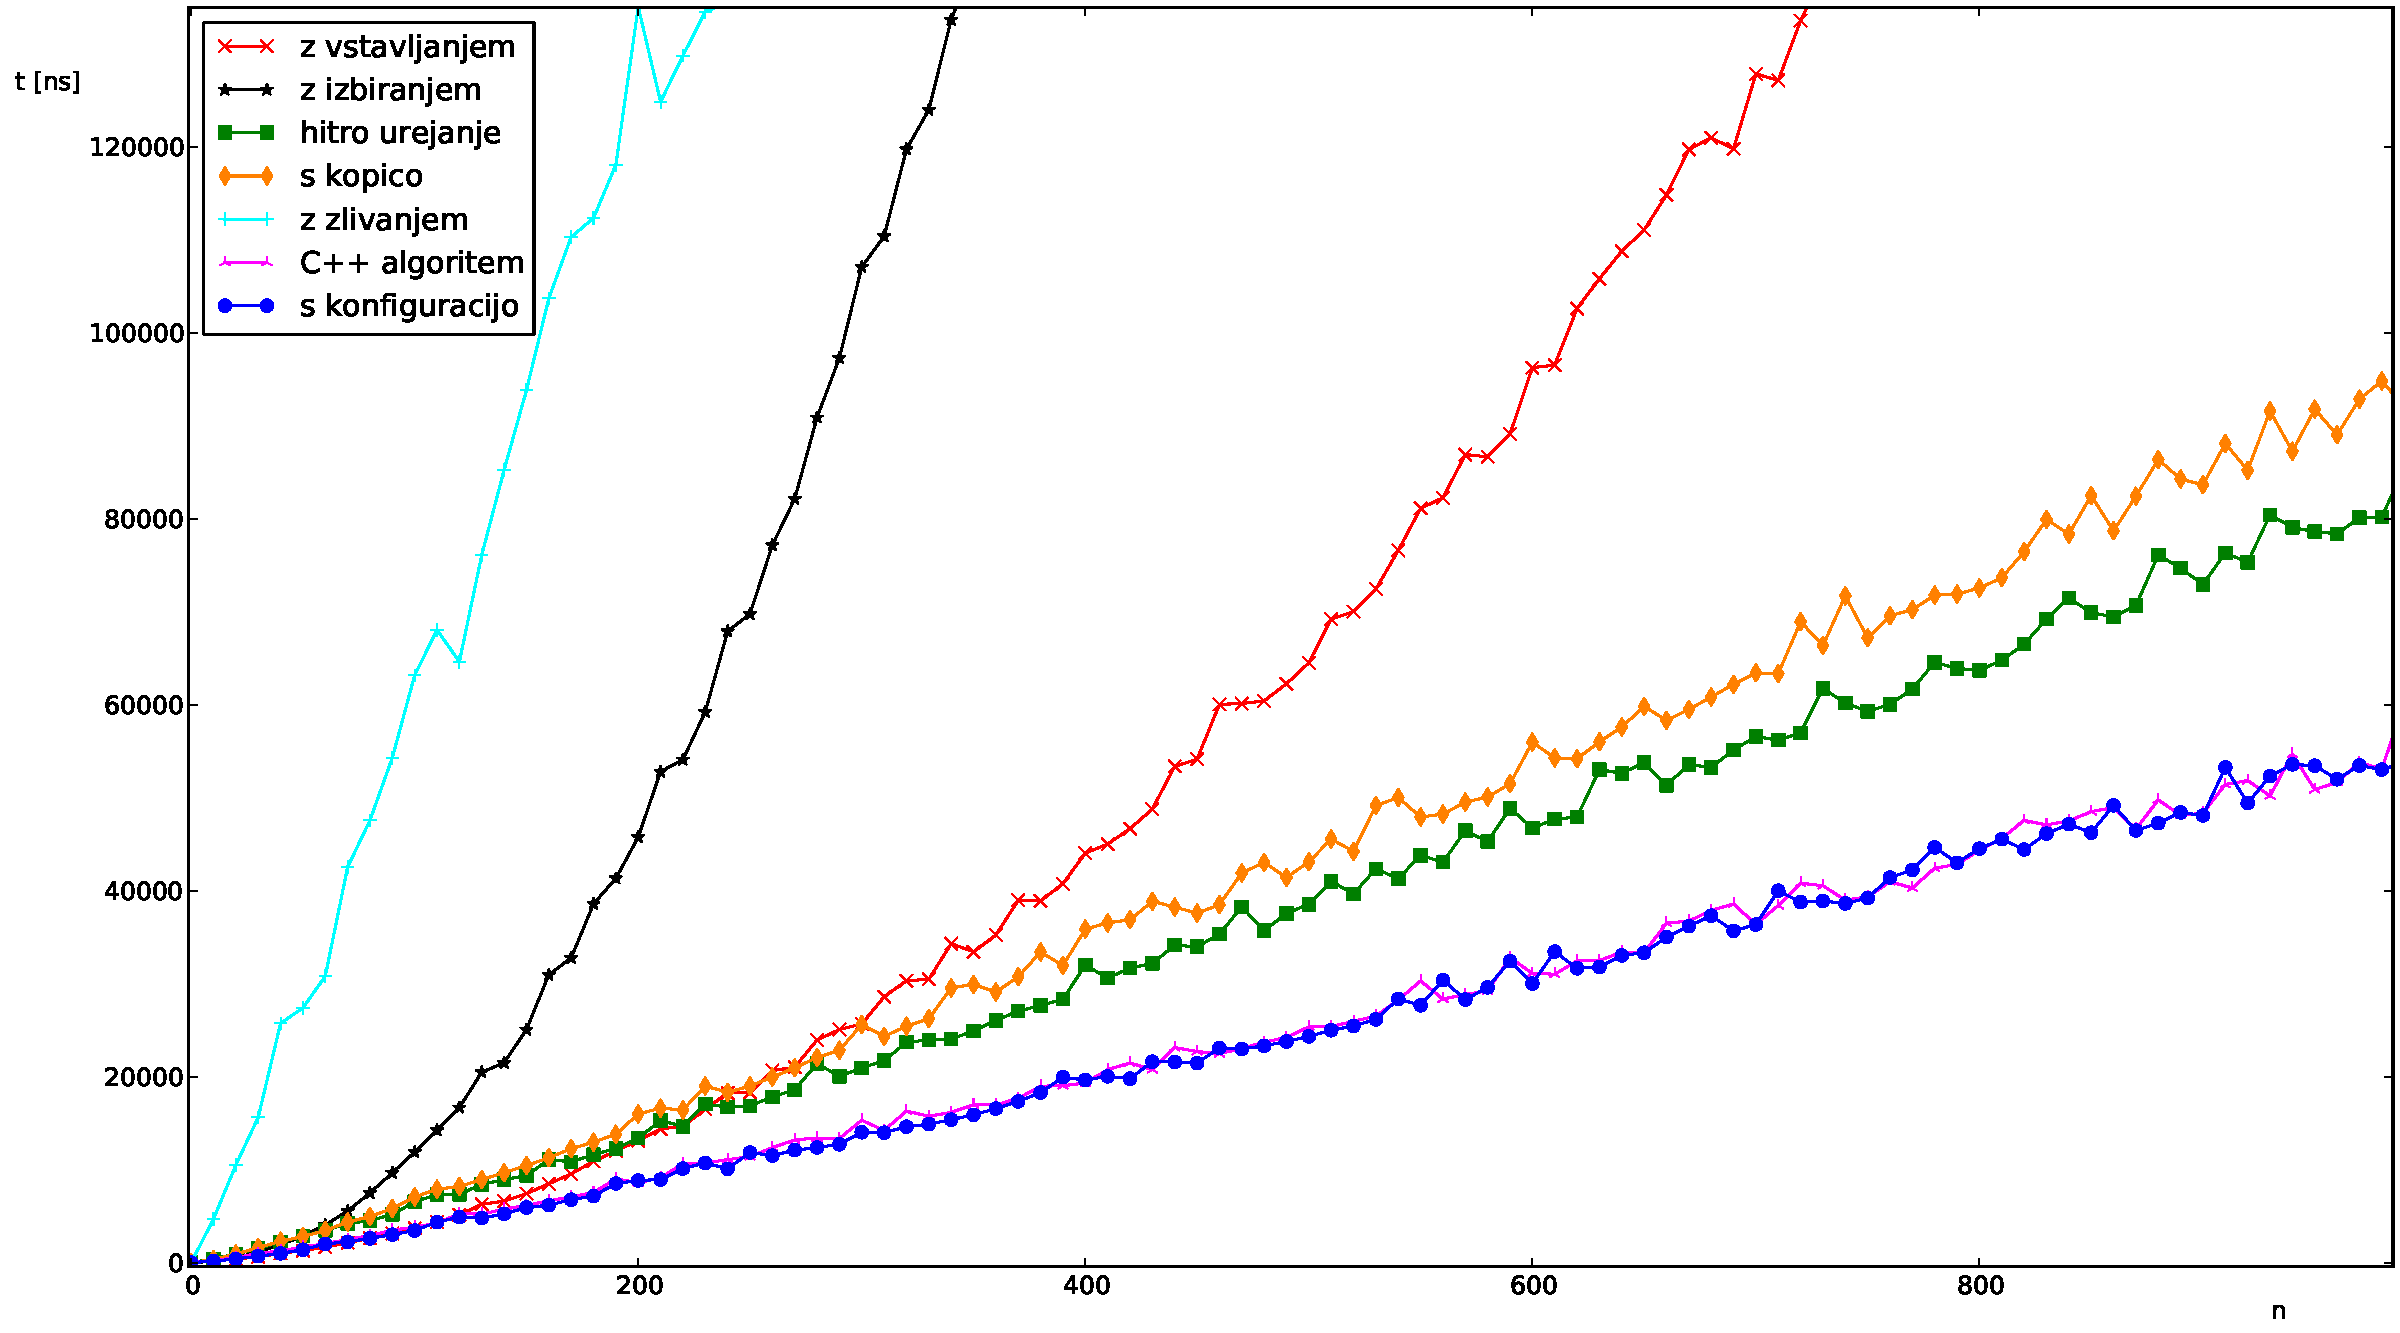
\includegraphics[width=\textwidth]{slike/int1000.pdf}
    \vspace{-0.7cm}
    \caption[Rezultati za tip \emph{int}, 1.000 el.]{Rezultati za tip \emph{int},
    1.000 elementov.}
    \caption*{{\small Graf prikazuje čase
    urejanja različnih sortirnih algoritmov v odvisnosti od dolžine polja. Polja
    so dolga od 1 do 1000 elementov. Za vsako dolžino polja je program naredil
    1.000 iteracij. Prikazan je le del grafa, da se vidi
    primerjava med učinkovitejšimi urejanji.}}
    \label{fig:rez:int1000}
\end{figure}

\begin{figure}[h!]
    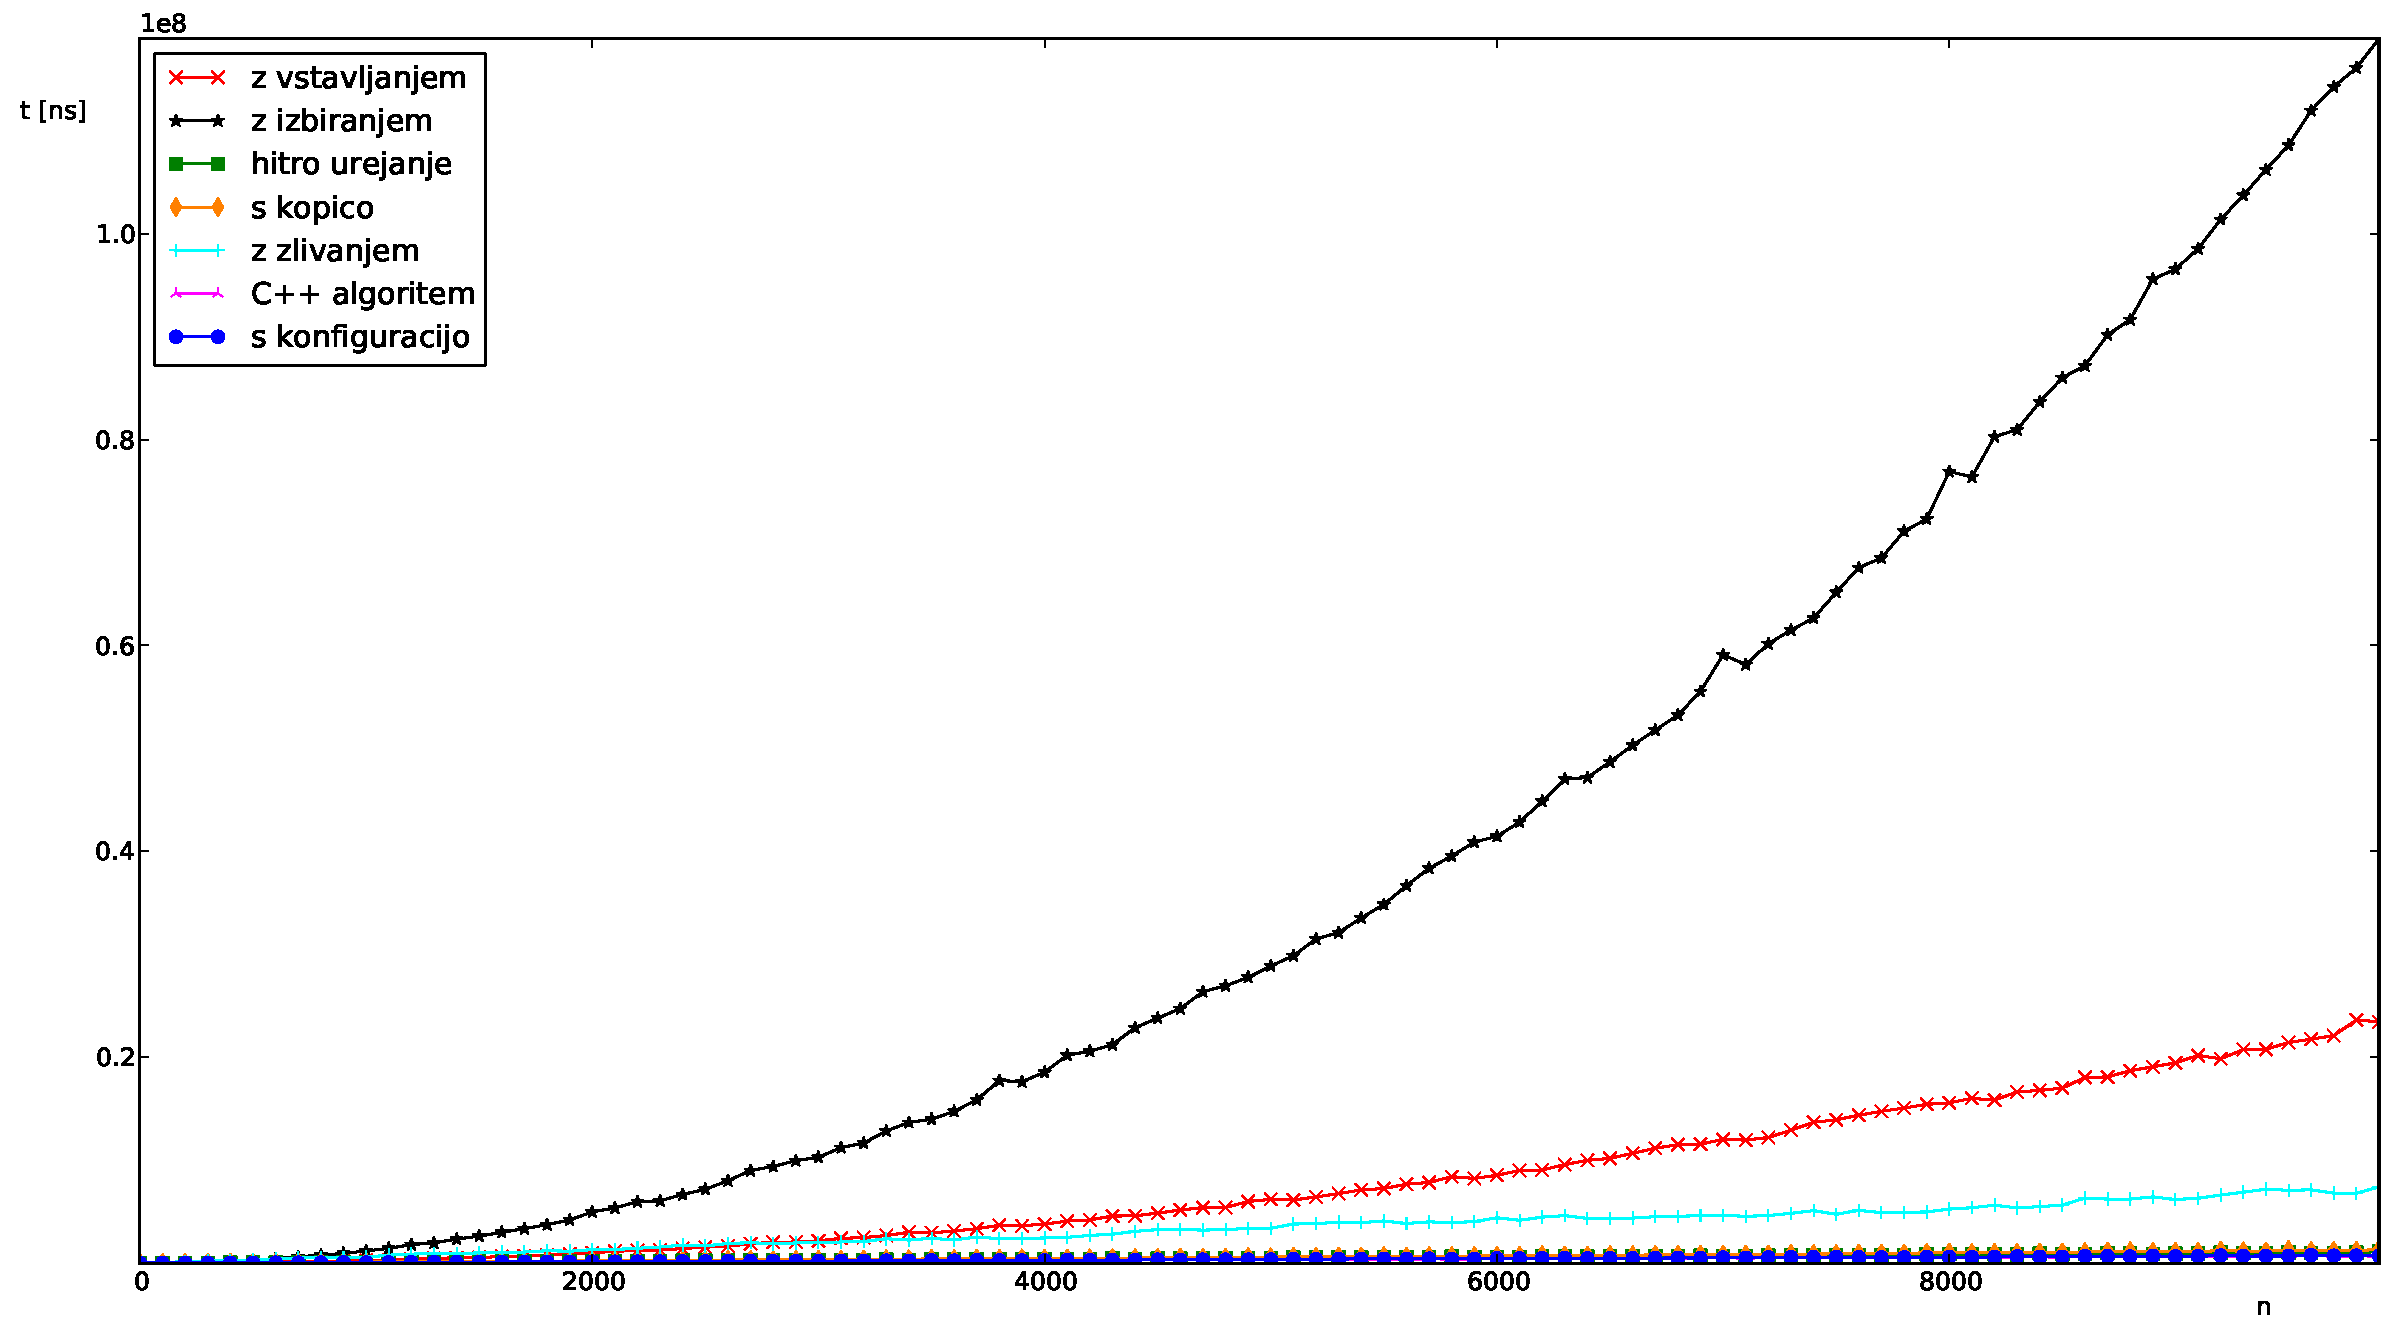
\includegraphics[width=\textwidth]{slike/int10000.pdf}
    \vspace{-0.7cm}
    \caption[Rezultati za tip  \emph{int}, 10.000 el.]{Rezultati za tip
    \emph{int}, 10.000 elementov.} 
    \caption*{{\small Graf prikazuje čase
    urejanja različnih sortirnih algoritmov v odvisnosti od dolžine polja, vse
    od dolžine 1 do 10.000. Program je za vsako dolžino polja naredil 100
    iteracij. Samo spodnji del grafa je prikazan na
    sliki~\ref{fig:rez:intblizu}.}}
    \label{fig:rez:int}
\end{figure}

\begin{figure}[h!]
    \begin{center}
        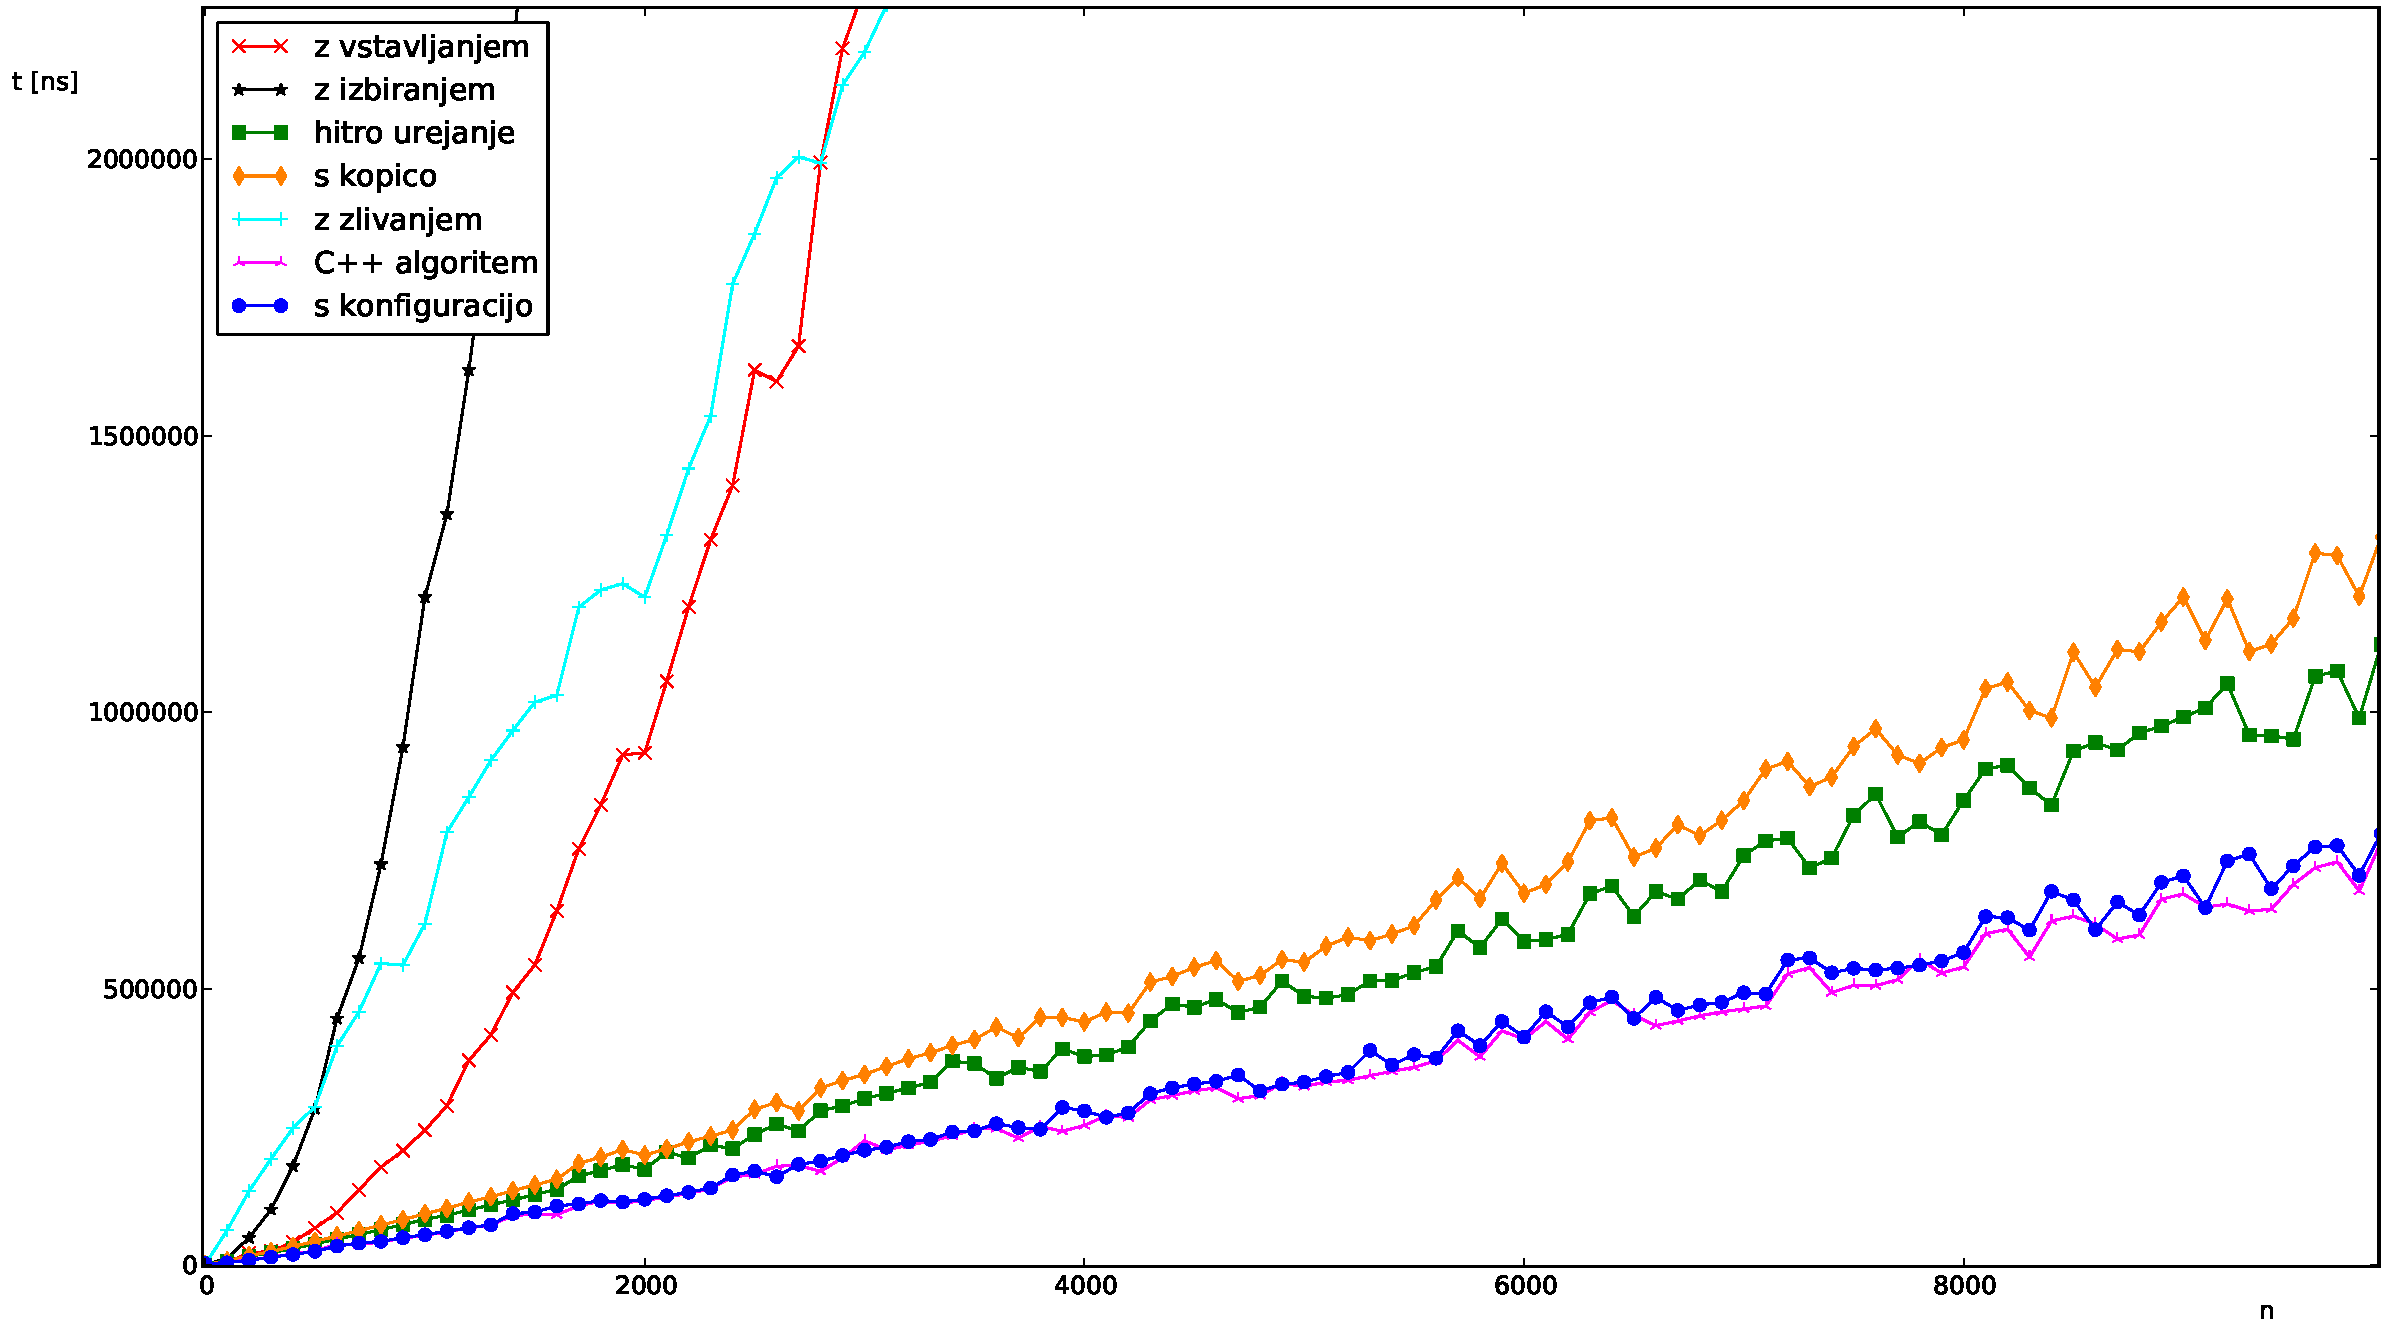
\includegraphics[width=\textwidth]{slike/int10000zoom.pdf}
    \end{center}
    \vspace{-0.7cm}
    \caption[Rezultati za tip \emph{int}, 10.000 el. -- izrez]{Prikazan
    spodnji del grafa na sliki~\ref{fig:rez:int}.} 
    \label{fig:rez:intblizu}
\end{figure}

\pagebreak
\mbox{}

\pagebreak
\subsection{Tip \emph{string}}
\label{chapter:rez:string}
Tip \emph{string} predstavlja niz znakov poljubne dolžine. Nizi, ki sem jih urejal, so
bili dolgi od enega do dvanajst znakov in so v pomnilniku zavzeli sorazmerno malo prostora
vendar več kot \emph{int}. Primerjava dveh nizov znakov lahko traja sorazmerno dolgo, saj se
nizi primerjajo leksikografsko, najprej po prvi črki, nato po drugi in tako vse do zadnje.
Primerjanje črke z drugo traja tako dolgo kot primerjanje dveh objektov tipa \emph{int}.
Primerjava dveh nizov znakov tako traja najmanj tako dolgo kot primerjava dveh števil, lahko
pa tudi veliko dlje, odvisno od števila enakih zaporednih črk med nizoma.

Najdena optimalna konfiguracija za kompozitni sortirni algoritem za tip \emph{string} je sledeča:
\[ :s \lra 5;:q \lra 3454;:m \lra 3844;:q \lra 4948; \] 
\[ :h \lra 6154;:m \lra 6530;:h \lra -1; \edot \]

\begin{table}[h!]
  \centering
  \caption[Rezultati za tip \emph{string}]{Rezultati za tip \emph{string.}}
  \label{tab:rez:string} \vspace{1ex}
  \begin{tabular}{l!{\vrule width 1pt}r|r|r|r}
    \bf št. elementov     & \bf 10 el.& \bf 100 el.& \bf 1.000 el. & \bf 10.000 el. \\ 
    \bf št. iteracij      & \bf 100.000 it. & \bf 10.000 it. & \bf 1.000 it. & \bf 100 it. \\ \hline
    \bf urejanje          & \bf čas [\usec] & \bf čas [\usec] & \bf čas [\usec] & \bf čas[\usec] \\ \noalign{\hrule height 1pt} 
    z vstavljanjem        & 2,24 & 160,40 & 18.925,12 & 2.077.954,54 \\ \hline
    z izbiranjem          & 1,53 & 151,75 & 18.456,58 & 2.146.882,90 \\ \hline
    hitro urejanje        & 2,44 &  44,26 &    704,11 &    15.663,25 \\ \hline
    s kopico              & 1,71 &  40,82 &    736,21 &    10.516,13 \\ \hline
    z zlivanjem           & 8,66 & 168,17 &  2.358,61 &    38.040,68 \\ \hline
    C++ algoritem         & 2,81 &  42,44 &    573,08 &     6.094,49 \\ \hline
    s konfiguracijo       & 1,55 &  35,78 &    644,23 &    10.576,94 \\ 
  \end{tabular}
\end{table}

\begin{table}[h!]
  \centering
  \caption[Skupen čas urejanja za tip \emph{string}]{Skupen čas urejanja za tip \emph{string.}}
  \caption*{{\small Skupne čase urejanja smo dobili tako, da za posamezen algoritem 
  seštejemo ordinate vseh točk na sliki~\ref{fig:rez:string10000}, ki prikazujejo čase tega
  sortirnega algoritma. Vrednosti so zaradi preglednosti urejene naraščajoče.}}
  \label{tab:rez:stringavegrage} \vspace{1ex}
  \begin{tabular}{|l|r|}
    \hline
    \bf sortirni algoritem   & \bf čas[ns], $\mathbf{1 \leq n \leq 10.000}$ \\ \noalign{\hrule height 1pt} 
    vgrajeni algoritem v C++ &    331.908.132 \\ \hline
    urejanje s konfiguracijo &    518.292.327 \\ \hline 
    urejanje s kopico        &    540.306.780 \\ \hline
    hitro urejanje           &    636.750.157 \\ \hline
    urejanje z zlivanjem     &  1.752.806.479 \\ \hline
    urejanje z vstavljanjem  & 72.328.942.517 \\ \hline
    urejanje z izbiranjem    & 74.442.461.661 \\ \hline
  \end{tabular}
\end{table}

\begin{figure}[h!]
    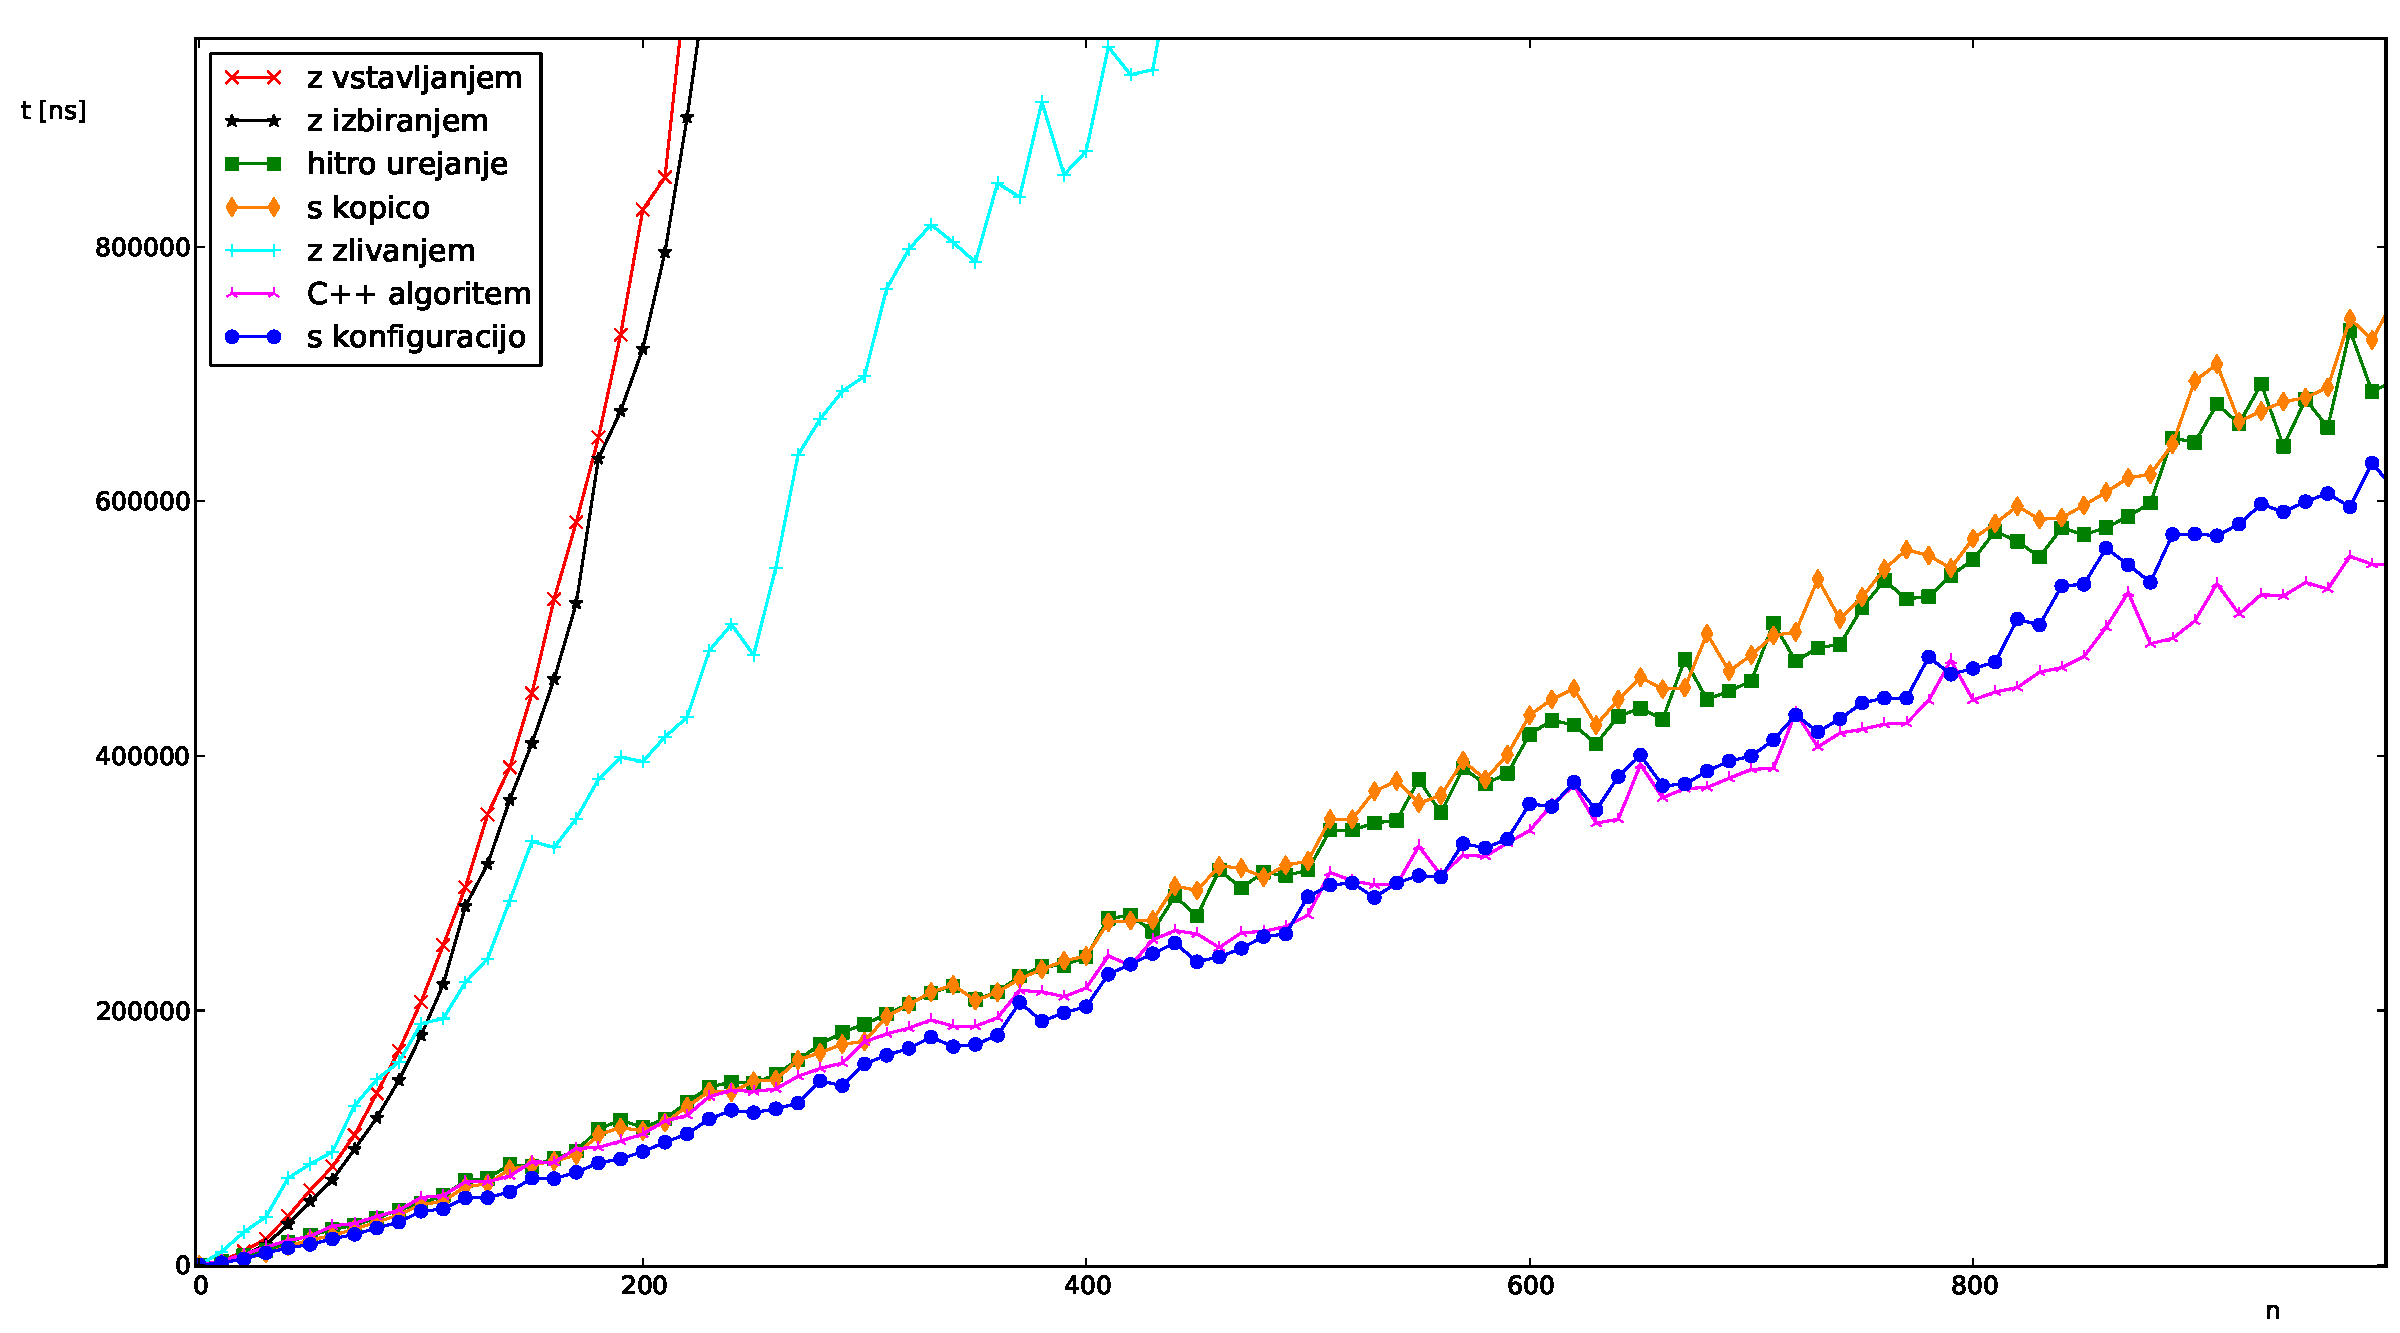
\includegraphics[width=\textwidth]{slike/string1000zoom.pdf}
    \vspace{-0.7cm}
    \caption[Rezultati za tip \emph{string}, 1.000 el. -- izrez]{Rezultati za tip
    \emph{string}, 1.000 elementov.}
    \caption*{{\small Graf prikazuje čase
    urejanja različnih sortirnih algoritmov za tip \emph{string} v odvisnosti od dolžine polja, vse
    od dolžine 1 do 1.000. Program je za vsako dolžino polja naredil 100
    iteracij. Približan je tako, da kaže zgolj popolne grafe učinkovitejših
    algoritmov, za boljšo primerjavo.}}
    \label{fig:rez:string1000}
\end{figure}

\begin{figure}[h!]
    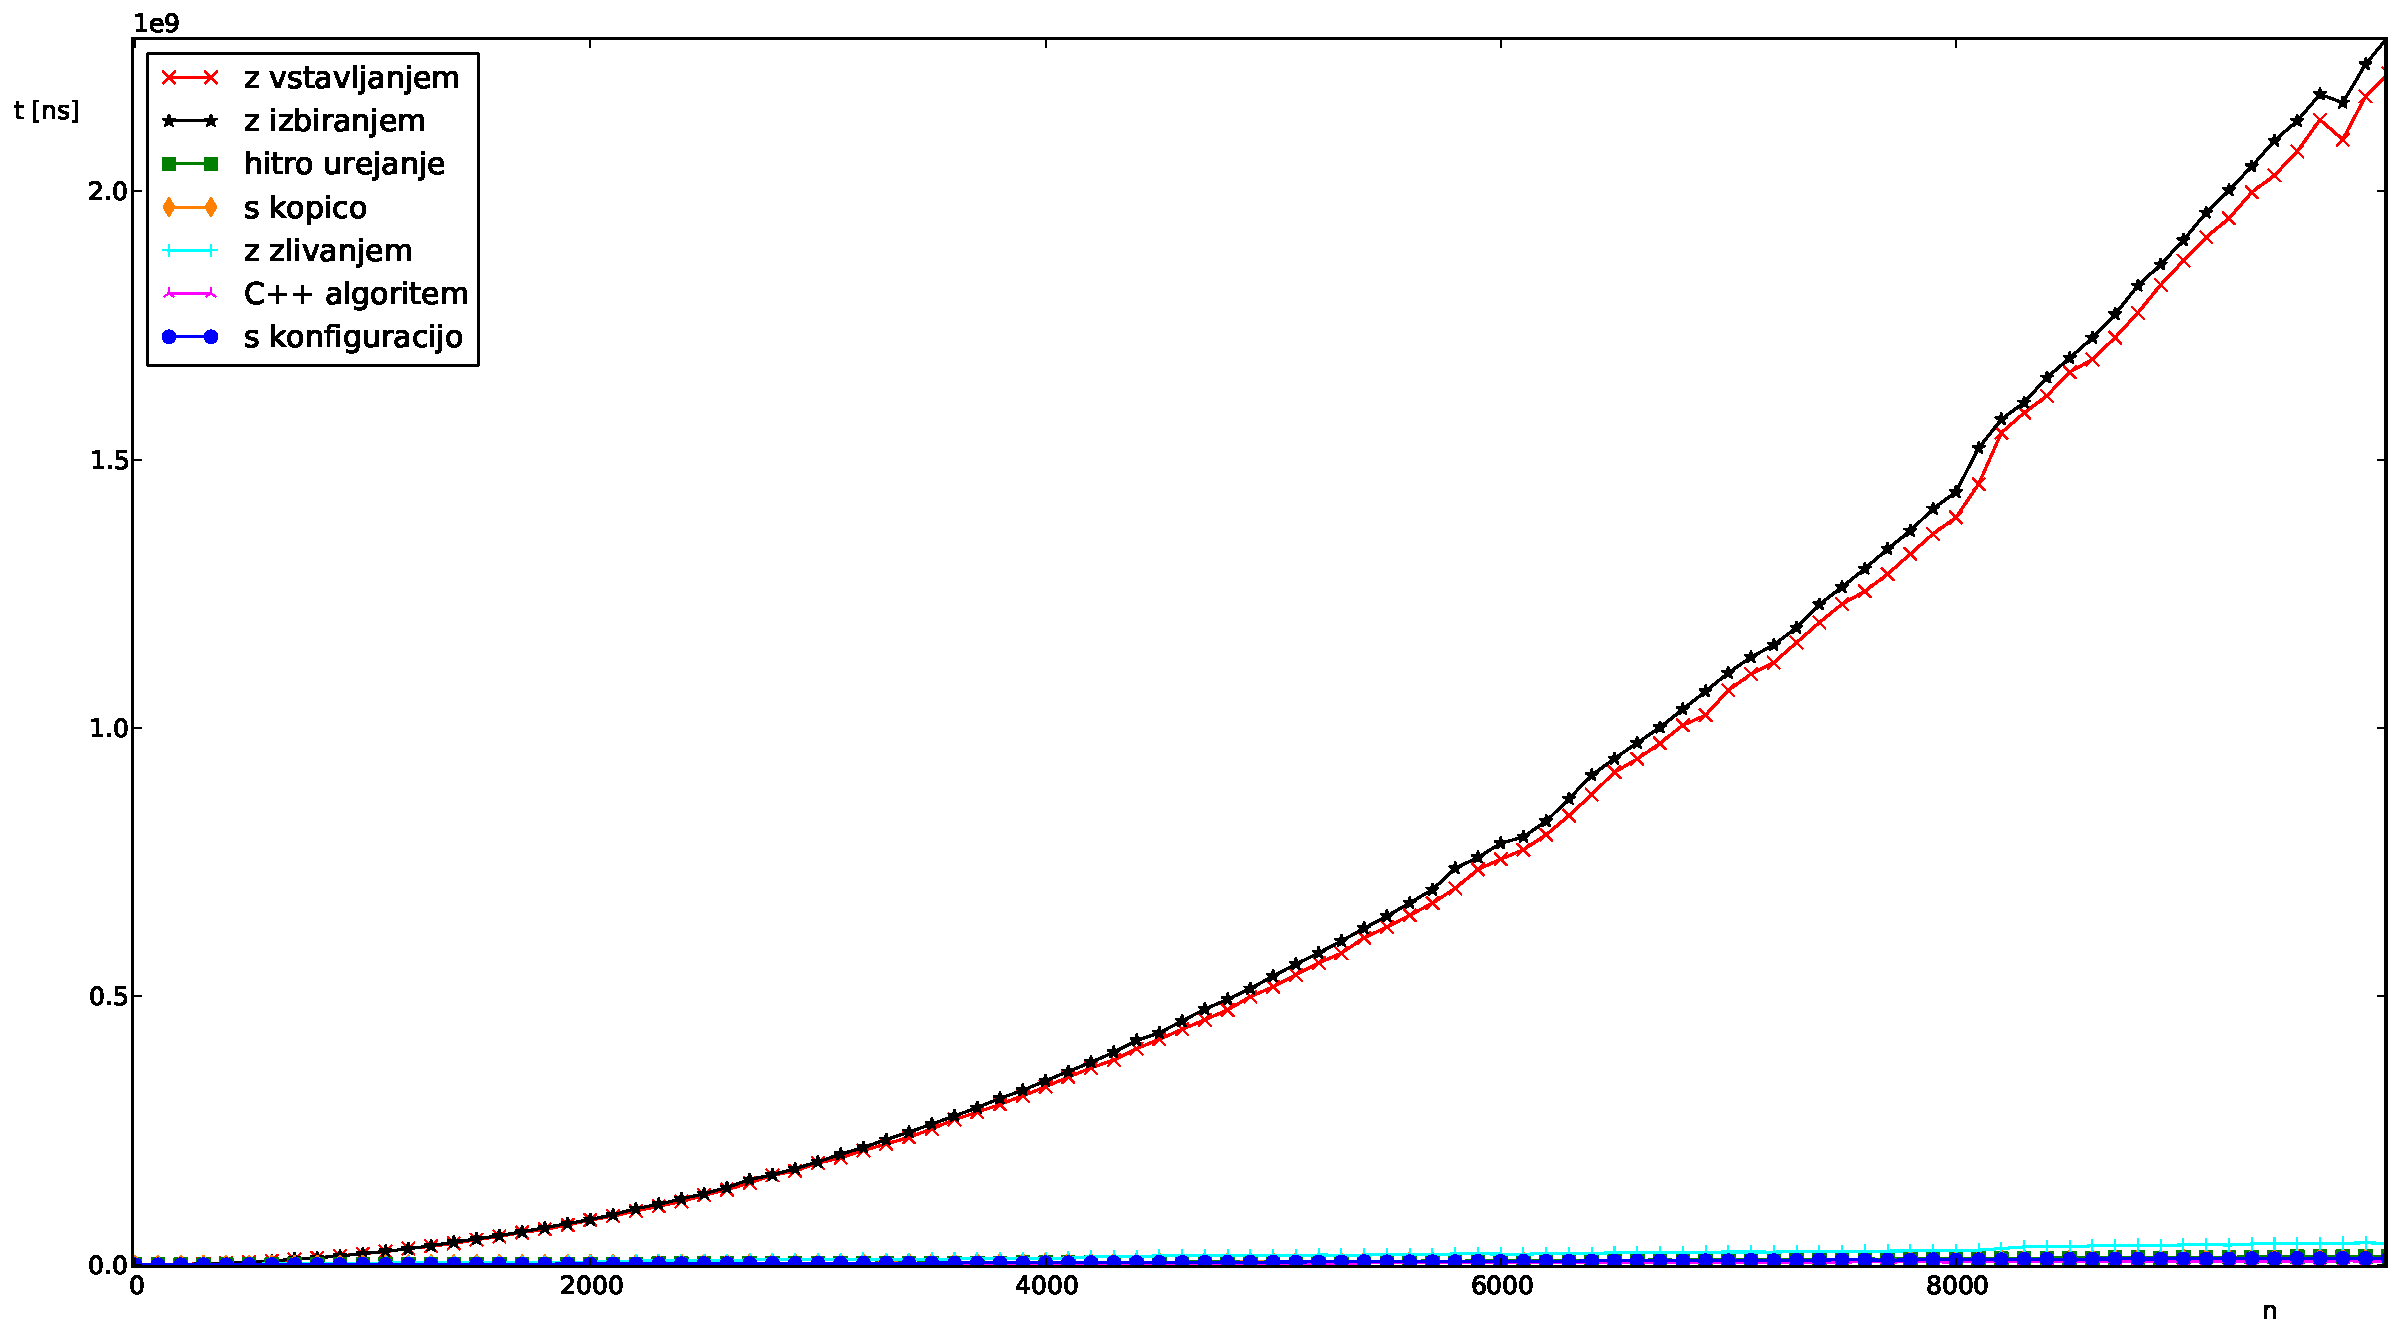
\includegraphics[width=\textwidth]{slike/string10000.pdf}
    \vspace{-0.7cm}
    \caption[Rezultati za tip \emph{string}, 10.000 el.]{Rezultati za tip
    \emph{string}, 10.000 elementov.}
    \caption*{{\small Graf prikazuje čase
    urejanja različnih sortirnih algoritmov za tip \emph{string} v odvisnosti od dolžine polja, vse
    od dolžine 1 do 10.000. Program je za vsako dolžino polja naredil 10
    iteracij. Spodnji del tega grafa je prikazan na
    sliki~\ref{fig:rez:string10000zoom}.}}
    \label{fig:rez:string10000}
\end{figure}

\begin{figure}[h!]
    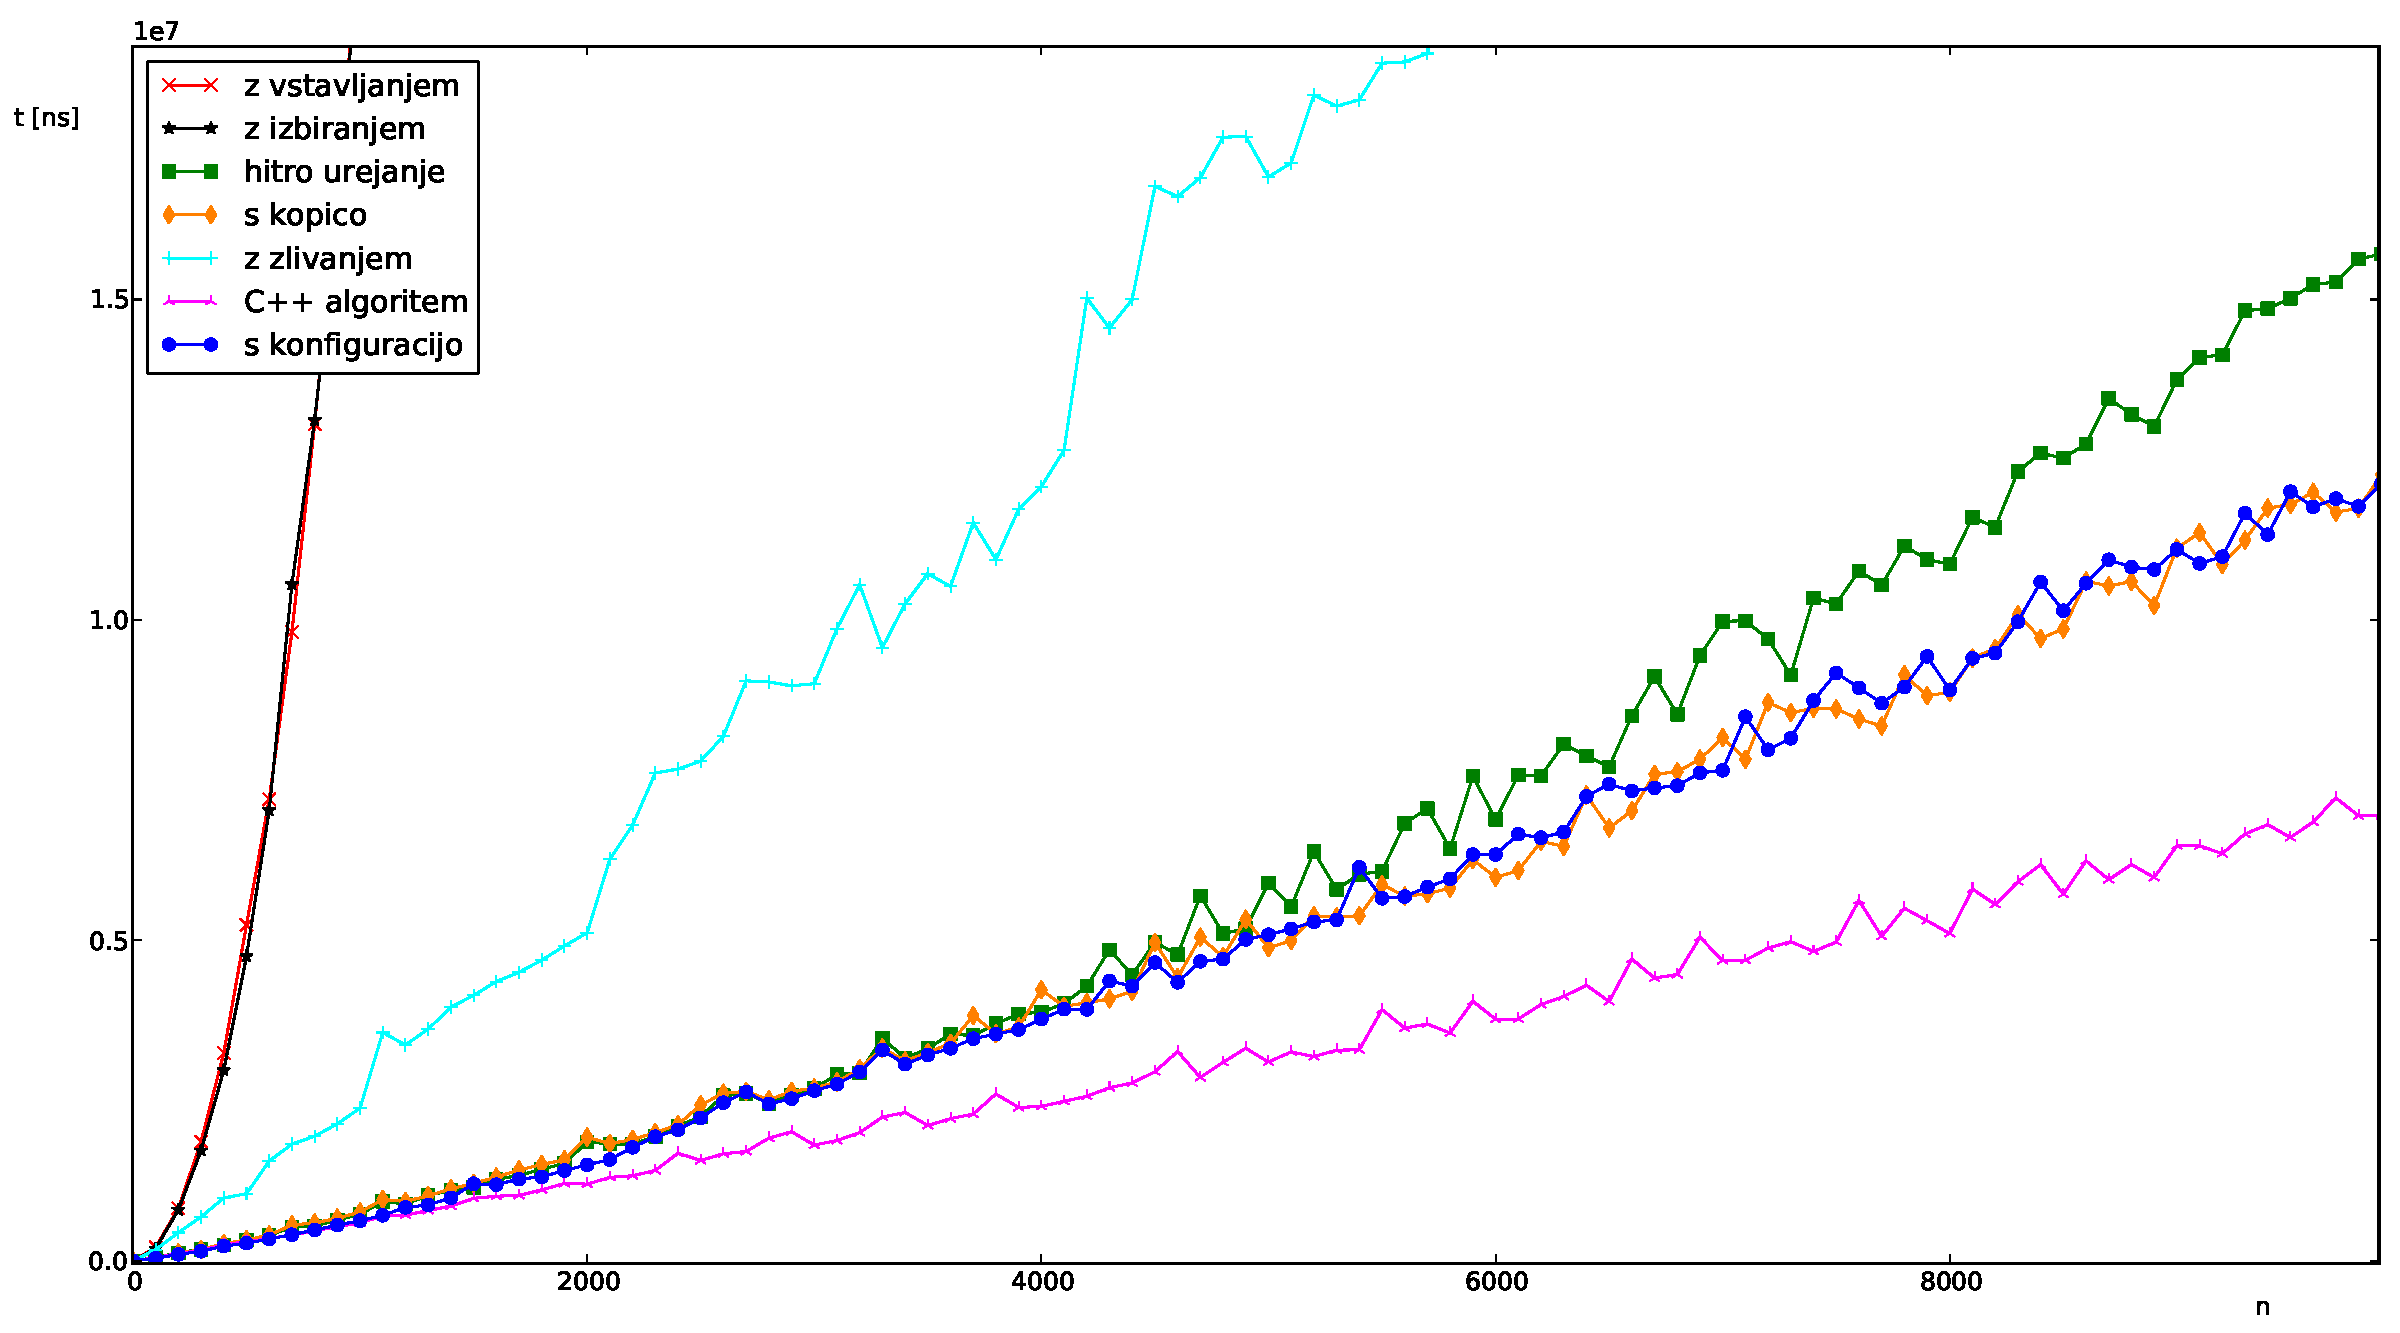
\includegraphics[width=\textwidth]{slike/string10000zoom.pdf}
    \vspace{-0.7cm}
    \caption[Rezultati za tip \emph{string}, 10.000 el. -- izrez]{Rezultati za
    tip \emph{string}, 10.000 elementov.}
    \caption*{{\small Slika prikazuje le spodnji del grafa na sliki~\ref{fig:rez:string10000},
    za boljšo primerjavo med učinkovitejšimi algoritmi.}}
    \label{fig:rez:string10000zoom}
\end{figure}

\pagebreak
\mbox{}

\pagebreak
\mbox{}

\pagebreak

\subsection{Tip \emph{huge}}
\label{chapter:rez:huge}
Tip \emph{huge} predstavlja uporabniški tip, katerega glavna lastnost je, da zavzame veliko pomnilnika.
Primerjava dveh objektov tega tipa traja tako dolgo kot primerjava dveh števil. Posamezen objekt
zavzame v pomnilniku veliko več prostora kot povprečen \emph{string} in zato tudi njegovo kopiranje 
traja dlje.

Najdena optimalna konfiguracija za kompozitni sortirni algoritem za tip \emph{huge} je sledeča:
\[ :i \lra 12;:s \lra 68;:q \lra 100;:s \lra 148;:q \lra 189;:s \lra 287;:q \lra -1; \edot \]

\begin{table}[h!]
  \centering
  \caption[Rezultati za tip \emph{huge}]{Rezultati za tip \emph{huge.}}
  \label{tab:rez:huge} \vspace{1ex}
  \begin{tabular}{l!{\vrule width 1pt}r|r|r|r}
    \bf št. elementov  & \bf 10 el.& \bf 100 el.& \bf 1.000 el. & \bf 10.000 el. \\ 
    \bf št. iteracij   & \bf 10.000 it. & \bf 1.000 it. & \bf 100 it. & \bf 10 it. \\ \hline
    \bf urejanje       & \bf čas [\usec] & \bf čas [\usec] & \bf čas [\usec] & \bf čas[\usec] \\ \noalign{\hrule height 1pt} 
    z vstavljanjem     &  5,32 & 306,65 & 41.567,63 & 13.789.989,83 \\ \hline
    z izbiranjem       &  5,57 &  89,48 &  2.034,52 &    177.534,11 \\ \hline
    hitro urejanje     &  6,21 & 102,77 &  1.386,03 &     23.740,07 \\ \hline
    s kopico           &  9,09 & 233,28 &  3.845,66 &     64.870,91 \\ \hline
    z zlivanjem        & 12,26 & 364,26 &  6.311,54 &    212.215,60 \\ \hline
    C++ algoritem      &  6,53 & 123,15 &  1.898,45 &     27.993,51 \\ \hline
    s konfiguracijo    &  5,78 &  77,41 &  1.215,61 &     21.840,79 \\ 
  \end{tabular}
\end{table}

\begin{table}[h!]
  \centering
  \caption[Skupen čas urejanja za tip \emph{huge}]{Skupen čas urejanja za tip \emph{huge.}}
  \caption*{{\small Skupen čas urejanja je pravzaprav vsota časov urejanja posameznega
  algoritma, ki so prikazani na grafu na sliki~\ref{fig:rez:huge1000}. 
  Vrednosti so zaradi preglednosti urejene naraščajoče.}}
  \label{tab:rez:hugeavegrage} \vspace{1ex}
  \begin{tabular}{|l|r|}
    \hline
    \bf sortirni algoritem   & \bf čas[ns], $\mathbf{1 \leq n \leq 1.000}$ \\ \noalign{\hrule height 1pt} 
    urejanje s konfiguracijo &   58.426.372,19 \\ \hline 
    hitro urejanje           &   67.858.490,70 \\ \hline
    urejanje z izbiranjem    &   75.267.185,97 \\ \hline
    vgrajeni algoritem v C++ &   81.821.545,08 \\ \hline
    urejanje s kopico        &  177.185.498,27 \\ \hline
    urejanje z zlivanjem     &  320.115.702,80 \\ \hline
    urejanje z vstavljanjem  & 1.341.428.566,28 \\ \hline
  \end{tabular}
\end{table}

\begin{figure}[h!]
    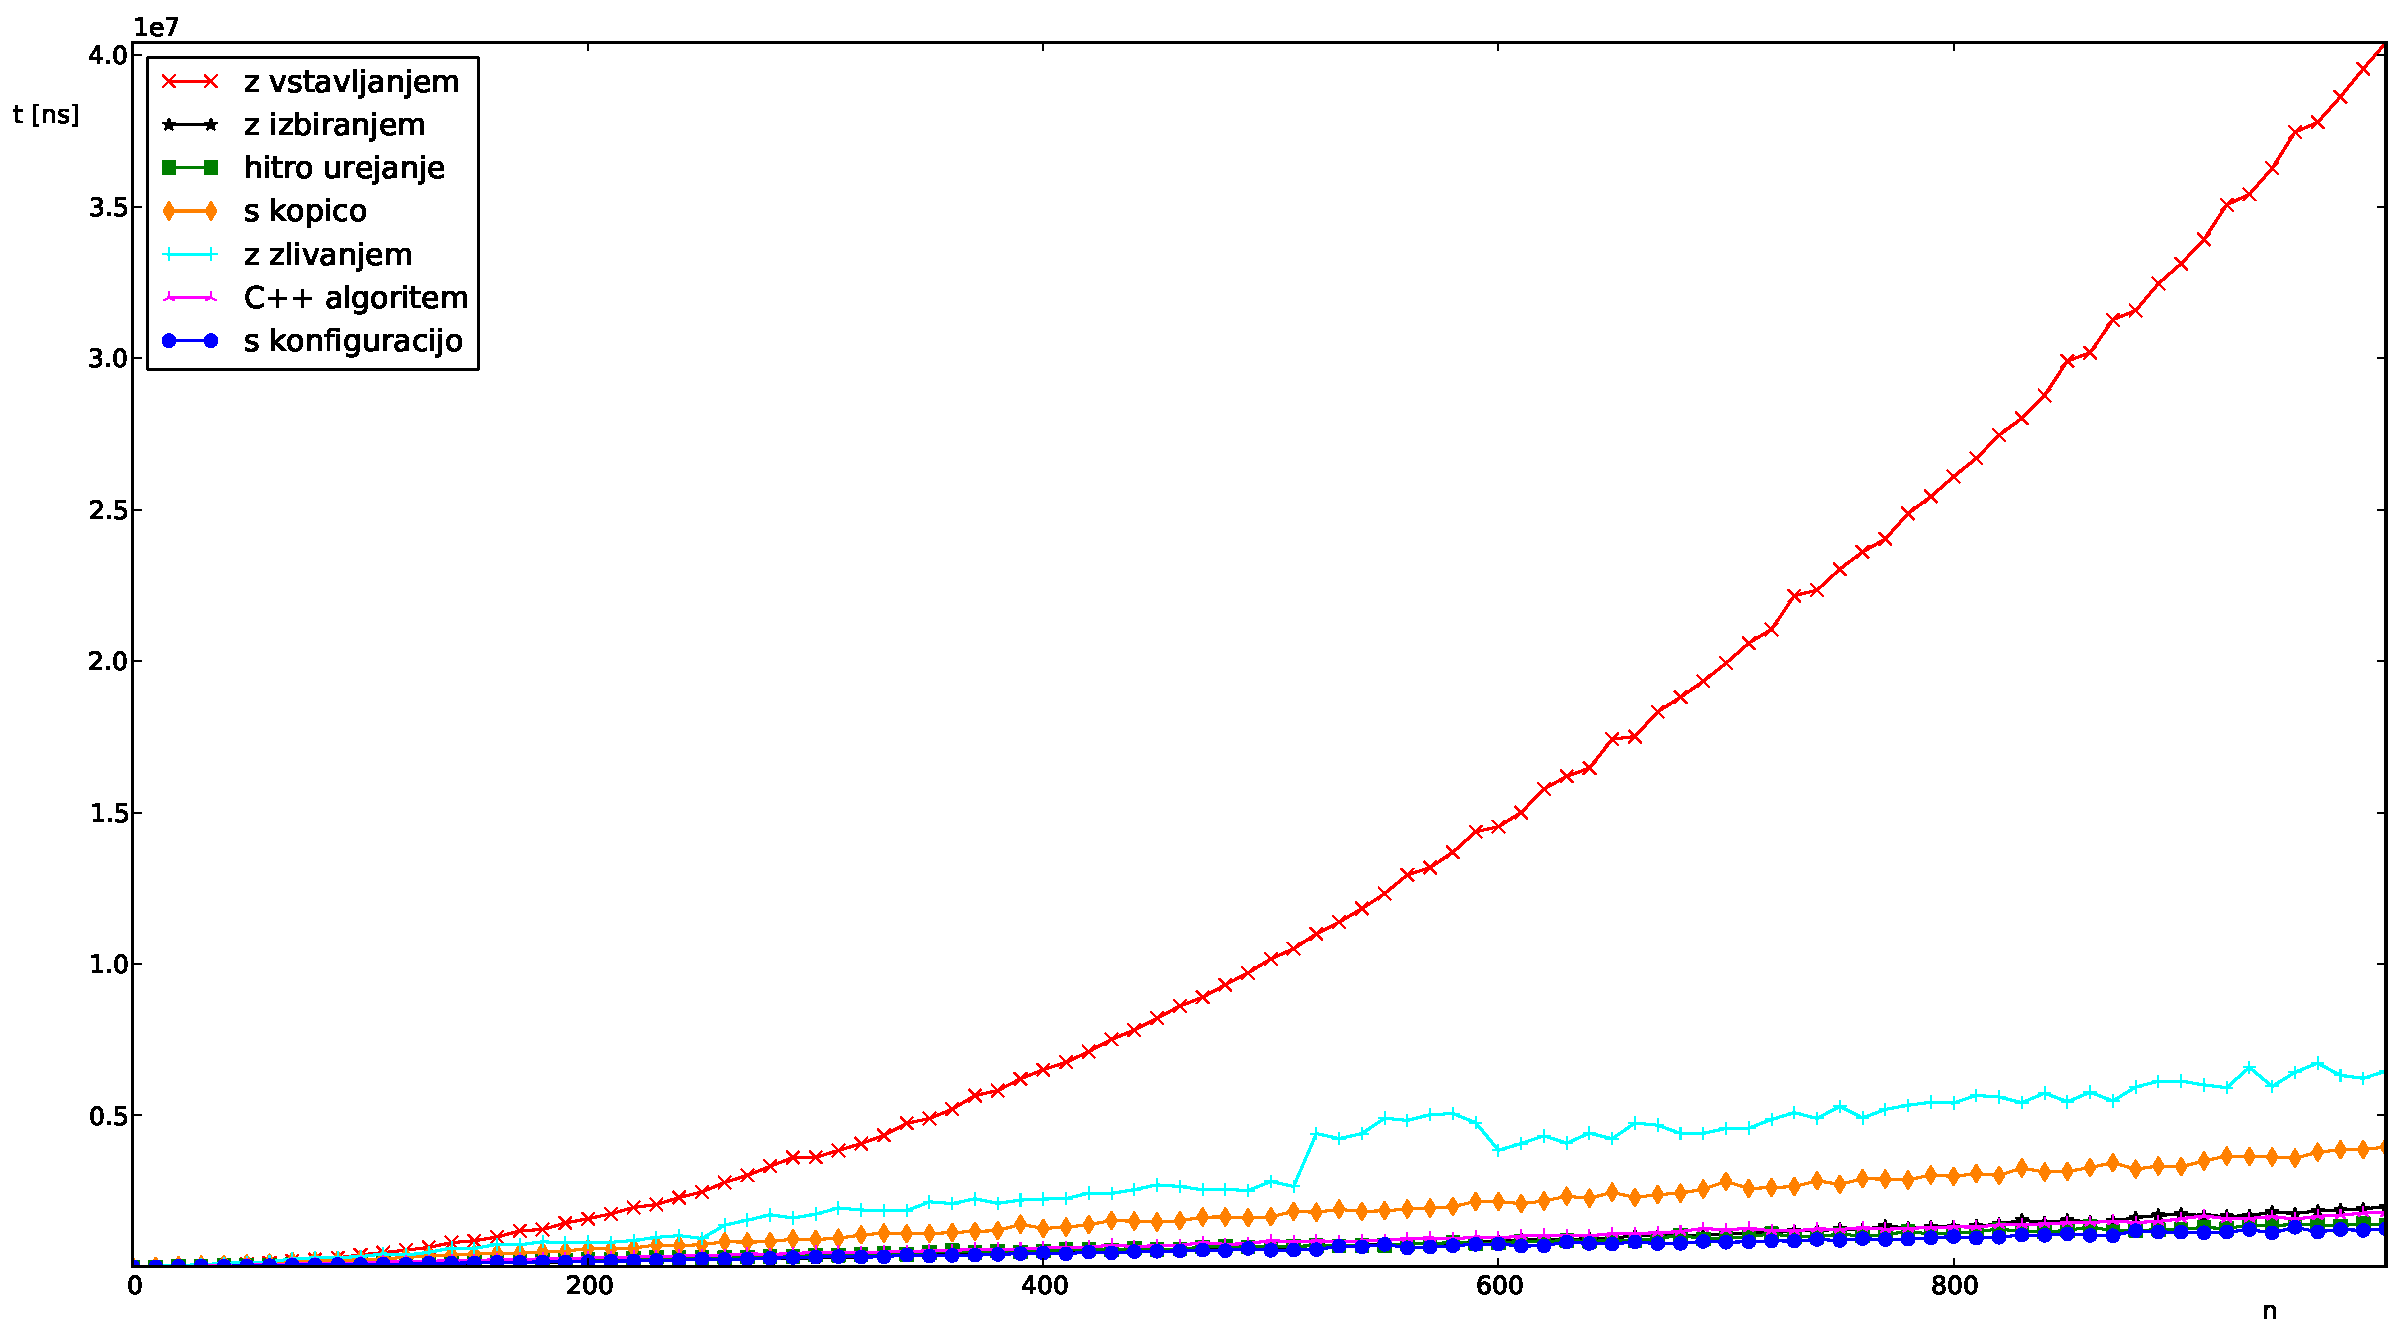
\includegraphics[width=\textwidth]{slike/huge1000.pdf}
    \vspace{-0.7cm}
    \caption[Rezultati za tip \emph{huge}, 1.000 el.]{Rezultati za tip
    \emph{huge} za polja z dolžino manjšo od 1000.}
    \caption*{{\small Graf prikazuje čase urejanja različnih sortirnih algoritmov
    za tip \emph{huge} v odvisnosti od dolžine polja, vse
    od dolžine 1 do 1000. Za vsako dolžino polja je program naredil 100 iteracij.
    Samo spodnji del grafa je prikazan na sliki~\ref{fig:rez:hugeblizu}.}}
    \label{fig:rez:huge1000}
\end{figure}

\begin{figure}[h!]
    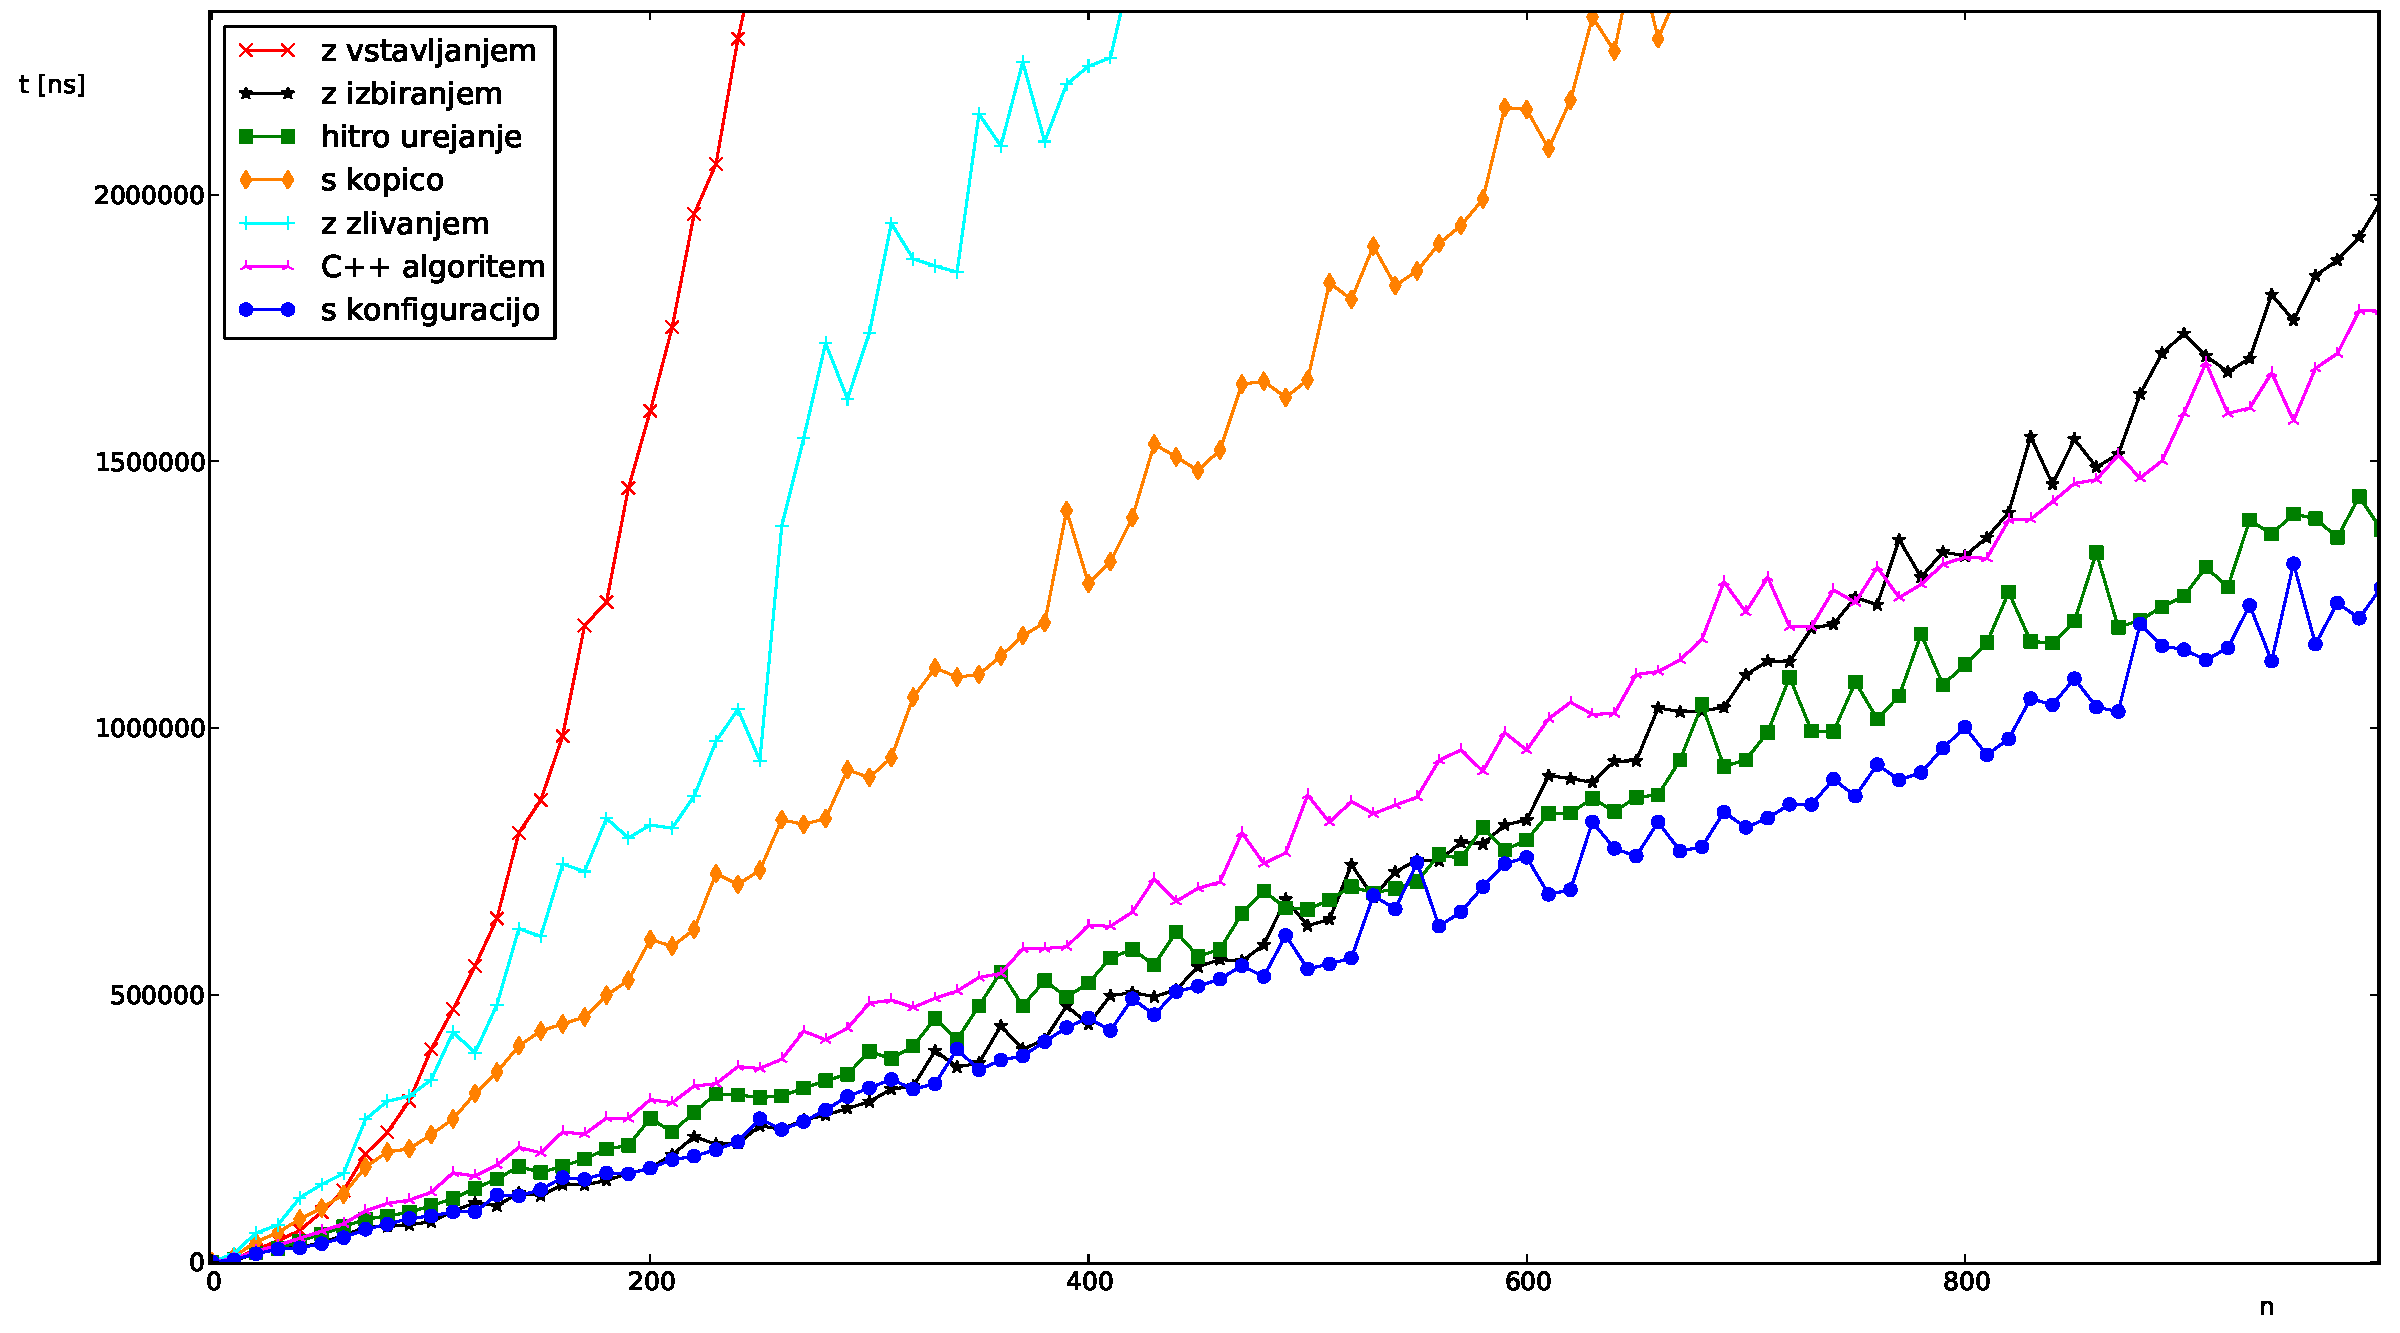
\includegraphics[width=\textwidth]{slike/huge1000zoom.pdf}
    \vspace{-0.7cm}
    \caption[Rezultati za tip \emph{huge}, 1.000 el. -- izrez]{Rezultati za tip
    \emph{huge}, 1.000 elementov.}
    \caption*{{\small Slika
    prikazuje samo spodnji del grafa na sliki~\ref{fig:rez:huge1000}, za
    boljšo primerjavo med učinkovitejšimi algoritmi.}}
    \label{fig:rez:hugeblizu}
\end{figure}

\pagebreak
\mbox{}

\pagebreak

\subsection{Tip \emph{slow}}
\label{chapter:rez:slow}
Tip \emph{slow} predstavlja uporabniški tip, katerega glavna lastnost je, da primerjanje dveh objektov
traja zelo dolgo. Primerjava dveh objektov tako traja veliko več časa kot primerjava dveh povprečnih
nizov znakov. V pomnilniku zavzame zelo malo prostora, približno toliko kot \emph{int}.

Najdena optimalna konfiguracija za kompozitni sortirni algoritem za tip \emph{slow} je sledeča:
\[ :i \lra 7;:m \lra -1; \edot \]

\begin{table}[h!]
  \centering
  \caption[Rezultati za tip \emph{slow}]{Rezultati za tip \emph{slow.}}
  \label{tab:rez:slow} \vspace{1ex}
  \begin{tabular}{l!{\vrule width 1pt}r|r|r|r}
    \bf št. elementov & \bf 10 el.& \bf 100 el.& \bf 1.000 el. & \bf 10.000 el. \\ 
    \bf št. iteracij  & \bf 10.000 it. & \bf 1.000 it. & \bf 100 it. & \bf 10 it. \\ \hline
    \bf urejanje      & \bf čas [\usec] & \bf čas [\usec] & \bf čas [\usec] & \bf čas[\usec] \\ \noalign{\hrule height 1pt} 
    z vstavljanjem    & 17,31 & 1.703,821 & 166.257,99 & 16.525.726,29 \\ \hline
    z izbiranjem      & 29,31 & 3.308,363 & 329.950,63 & 33.201.205,85 \\ \hline
    hitro urejanje    & 39,48 &   749,242 &  10.871,17 &   146.598,49  \\ \hline
    s kopico          & 24,97 &   681,290 &  11.211,39 &   157.949,93  \\ \hline
    z zlivanjem       & 18,33 &   400,140 &   6.117,13 &    85.727,57  \\ \hline
    C++ algoritem     & 20,37 &   506,029 &   7.745,60 &   105.082,31  \\ \hline
    s konfiguracijo   & 16,75 &   382,914 &   5.973,63 &    83.143,84  \\ 
  \end{tabular}
\end{table}

\begin{table}[h!]
  \centering
  \caption[Skupen čas urejanja za tip \emph{slow}]{Skupen čas urejanja za tip
  \emph{slow}.}
  \caption*{{\small Skupen čas urejanja za vsak posamezen algoritem dobimo
  tako, da seštejemo čase, ki jih je porabil pri vsakem $n$ posebej. Skupen čas
  urejanja pravzaprav predstavlja približek ploščine, ki jo na določenem intervalu omejita
  graf soritrnega algoritma in abscisna os na grafu na sliki~\ref{fig:rez:slow1000}.
  Vrednosti so zaradi preglednosti urejene naraščajoče.}}
  \label{tab:rez:slowavegrage} \vspace{1ex}
  \begin{tabular}{|l|r|}
    \hline
    \bf sortirni algoritem   & \bf čas[ns], $\mathbf{1 \leq n \leq 1.000}$ \\ \noalign{\hrule height 1pt} 
    urejanje s konfiguracijo &    275.974.571,31 \\ \hline 
    urejanje z zlivanjem     &    281.640.609,23 \\ \hline
    vgrajeni algoritem v C++ &    353.613.310,76 \\ \hline
    hitro urejanje           &    501.905.163,63 \\ \hline
    urejanje s kopico        &    505.171.708,97 \\ \hline
    urejanje z vstavljanjem  &  5.427.392.234,82 \\ \hline
    urejanje z izbiranjem    & 10.826.003.228,79 \\ \hline
  \end{tabular}
\end{table}


\begin{figure}[h!]
    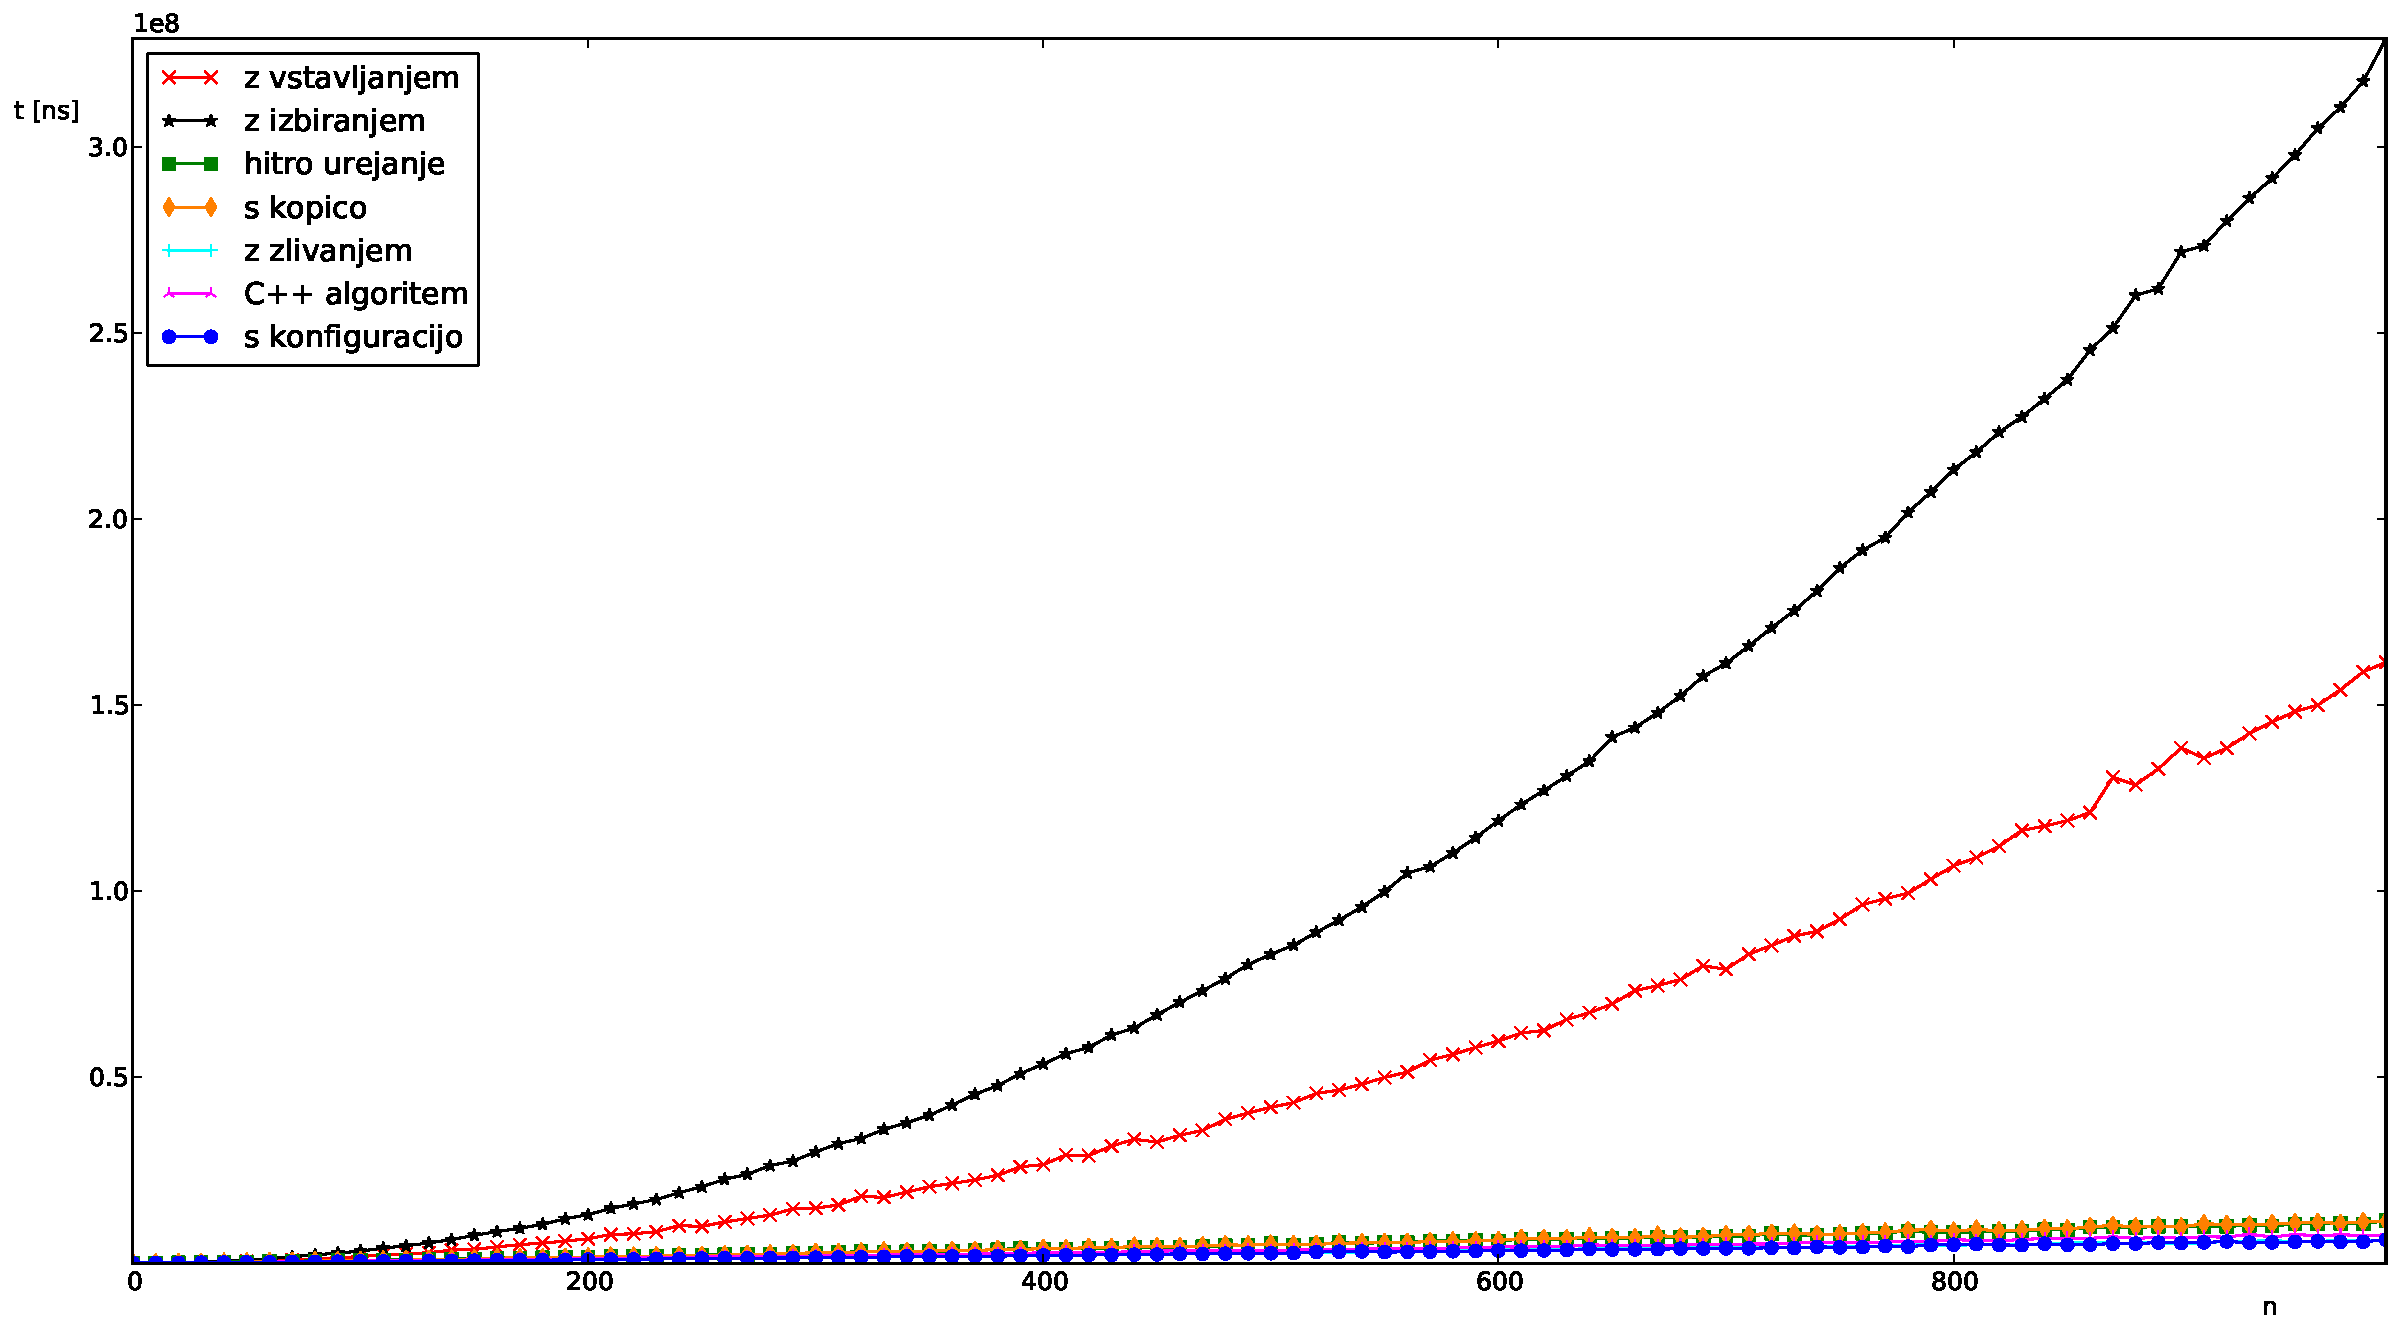
\includegraphics[width=\textwidth]{slike/slow1000.pdf}
    \vspace{-0.7cm}
    \caption[Rezultati za tip \emph{slow}, 1.000 el.]{Rezultati za tip
    \emph{slow} za polja z dolžino manjšo od 1.000.}
    \caption*{{\small Graf prikazuje čase
    urejanja različnih sortirnih algoritmov za tip \emph{slow} v odvisnosti od dolžine polja, vse
    od dolžine 1 do 1000. Za vsako dolžino polja je program naredil 10 iteracij.
    Samo spodnji del grafa je prikazan na sliki~\ref{fig:rez:slowblizu}.}}
    \label{fig:rez:slow1000}
\end{figure}

\begin{figure}[h!]
    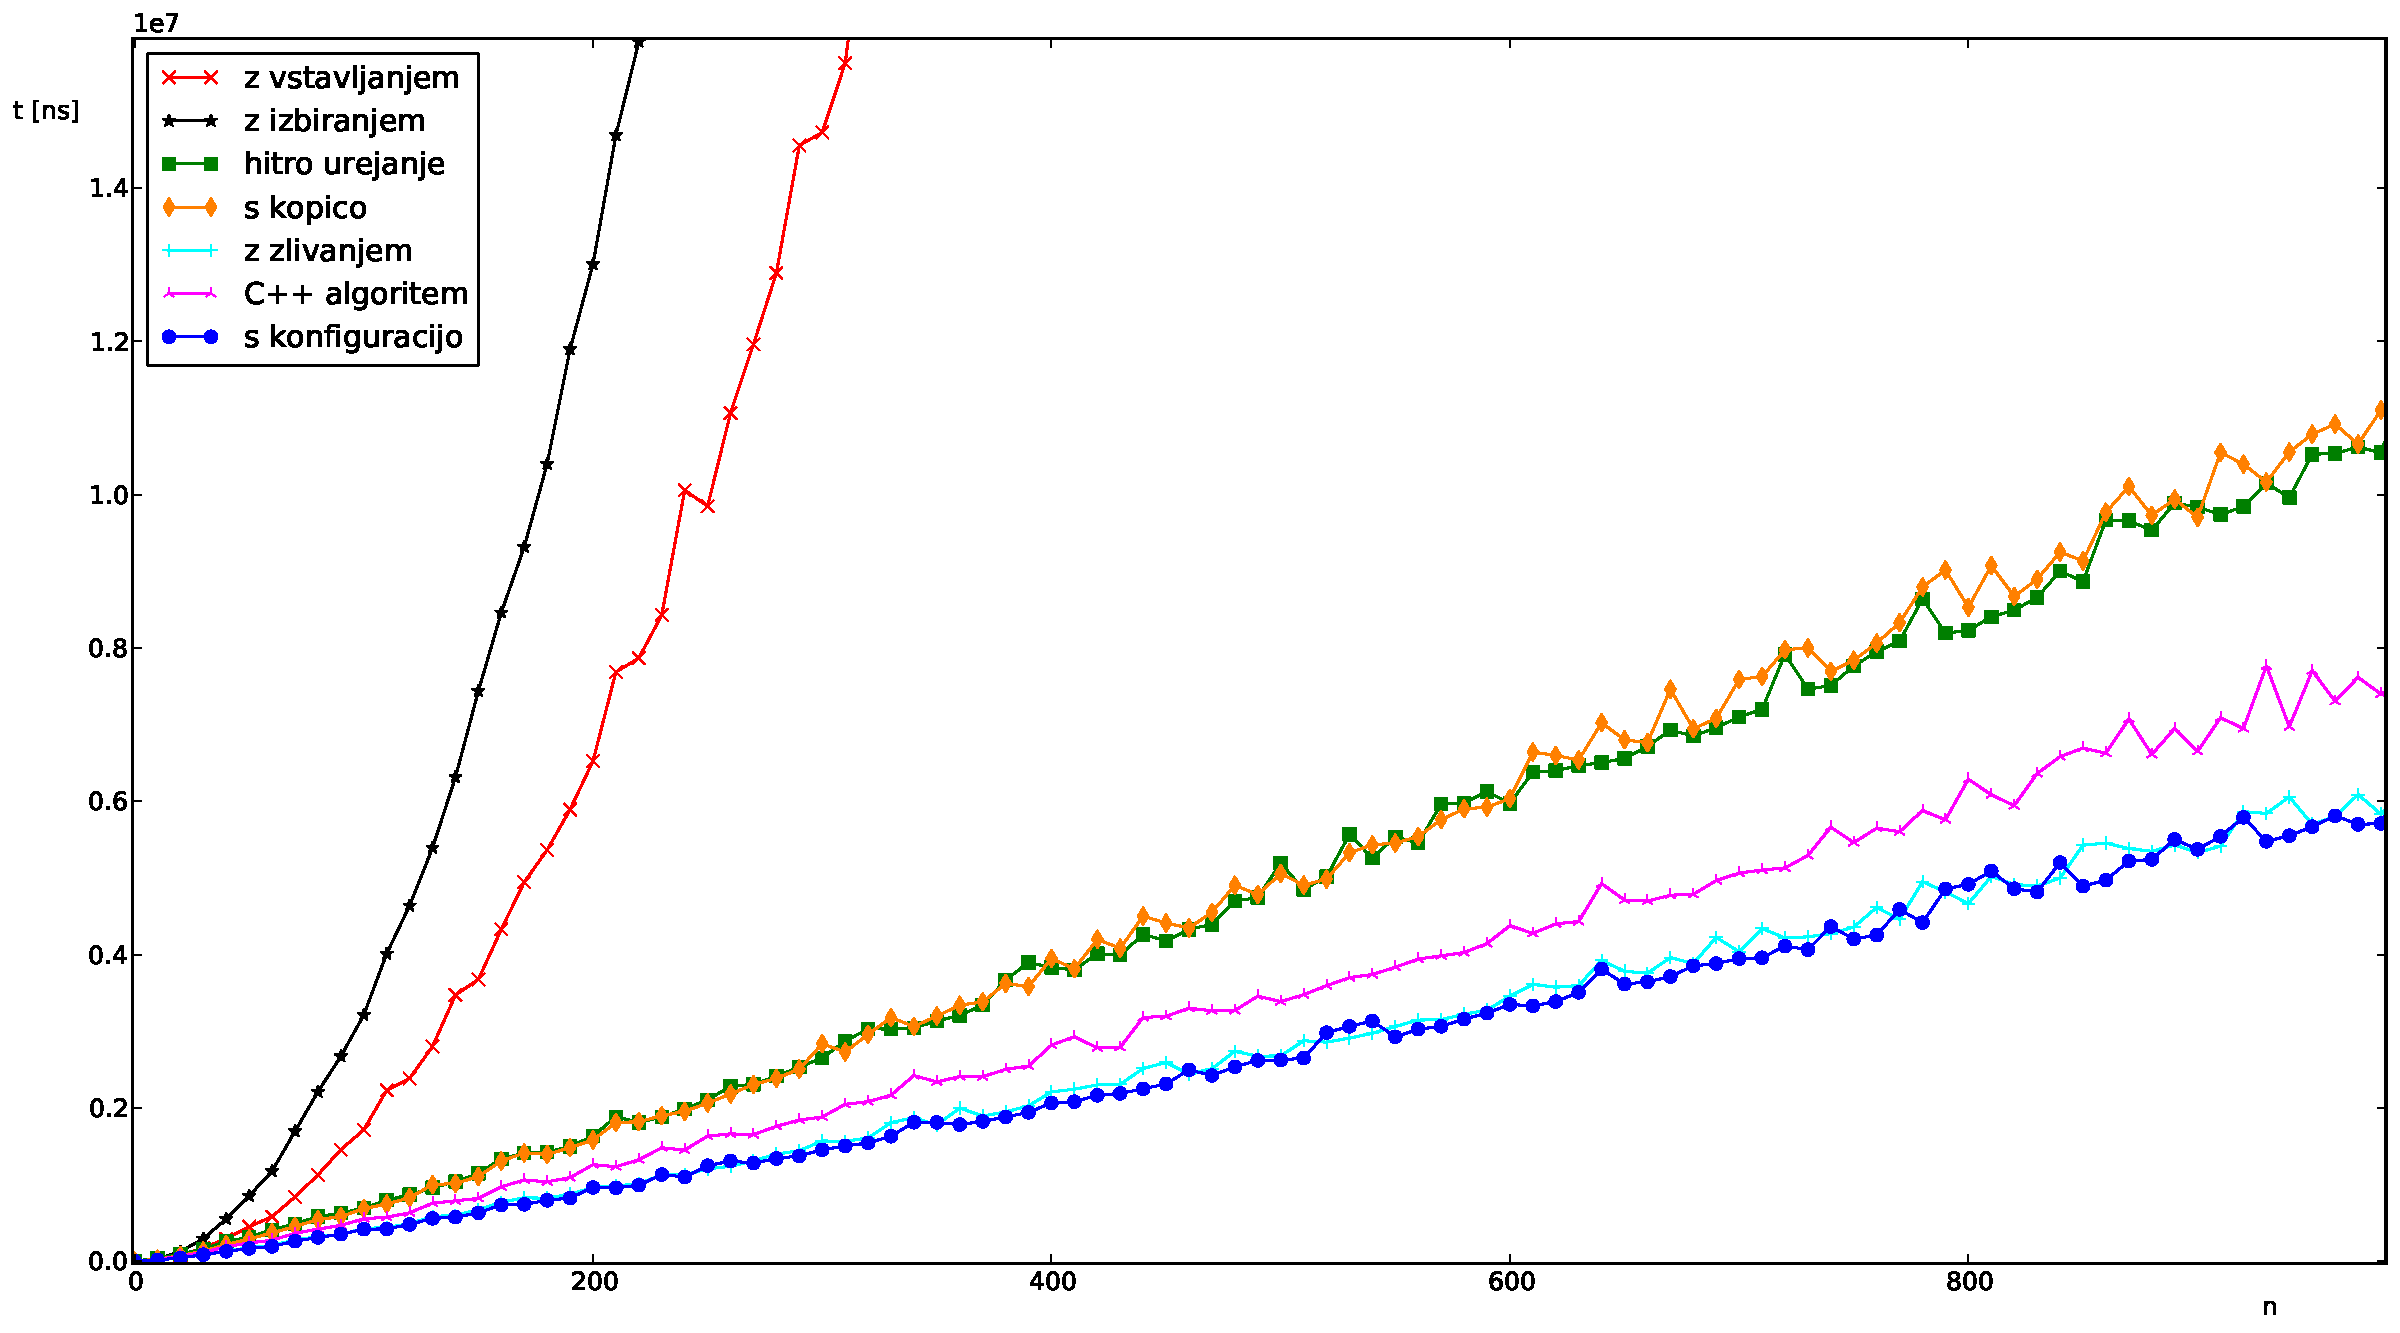
\includegraphics[width=\textwidth]{slike/slow1000zoom.pdf}
    \vspace{-0.7cm}
    \caption[Rezultati za tip \emph{slow}, 1.000 el. -- izrez]{Slika
    prikazuje zgolj spodnji del grafa na sliki~\ref{fig:rez:slow1000}, za
    boljšo primerjavo med učinkovitejšimi algoritmi. }
    \label{fig:rez:slowblizu}
\end{figure}

\pagebreak
\mbox{}

\pagebreak

\section{Ugotovitve in razprava}
\subsection{Tip \emph{int}}
Dobljena konfiguracija $:s \lra 5;:i \lra 67;:q \lra -1;$
se ujema s teoretičnim delom. Urejanje z izbiranjem in urejanje z vstavljanjem sta 
dobra na kratkih poljih, na daljših poljih pa je boljše hitro urejanje, kot zelo hiter algoritem na naključno
porazdeljenih podatkih. 

Rezultati v tabeli~\ref{tab:rez:int} za dolžino 10 kažejo podobno sliko. Urejanje z izbiranjem in urejanje 
z vstavljanjem sta boljša od vseh ostalih sortirnih algoritmov, urejanje s konfiguracijo in \mbox{C++-ov} 
algoritem, ki je prav tako kompoziten, sta za spoznanje slabša. Pri urejanju s konfiguracijo je to posledica
iskanja po konfiguraciji, česar urejanju z vstavljanjem ni potrebno delati. Sicer 
se urejanje s konfiguracijo obnaša popolnoma enako kot urejanje z vstavljanjem, saj vidimo, da se polja dolžine 
10 urejajo z le-tem. Urejanje z zlivanjem je pri tej dolžini daleč najslabše, saj naredi veliko 
rekurzivnih klicev in kopiranja elementov, kar je pri tako kratki dolžini zelo zamudno.

Pri stotih elementih se vrstni red že spremeni. Močno nazaduje urejanje z izbiranjem zaradi 
kvadratne časovne zahtevnosti tudi v najboljšem primeru. Urejanje z vstavljanjem je še vedno 
na prvem mestu med nekompozitnimi algoritmi, medtem ko se pri urejanju s konfiguracijo že kaže njegova
kompozitna narava, saj pri poljih dolžine 100 že uporablja hitro urejanje, ki polja razdeli na 
manjša podpolja, ki se potem, ko je njihova dolžina manjša ali enaka 67, uredijo z vstavljanjem.
Tako dosežemo hitrejše urejanje, kar se pozna že pri 100 elementih. Urejanje z zlivanjem je še 
vedno na zadnjem mestu, saj število elementov še ni dovolj veliko, da bi se vsi rekurzivni klici 
in kopiranje elementov splačali. Tudi na sliki~\ref{fig:rez:int1000} se vidijo
podobne ugotovitve. Urejanje z zlivanjem in urejanje z izbiranjem sta zelo
počasna (na sliki ravno ujamemo njuno presečišče), 
sledi jima urejanje z izbiranjem, sledita urejanje s kopico in tik na
njih hitro urejanje.  \mbox{C++-ov} algoritem in urejanje s konfiguracijo se praktično
prekrivata, vendar je urejanje s konfiguracijo za približno $n < 600$ zagotovo
boljše od \mbox{C++-ovega} algoritma, za $n$-je večje od 600 pa v večini primerov, a že
vidimo, da se približuje njuno presečišče.

Pri tisočih elementih pa se že pokaže pričakovana časovna zahtevnost algoritmov. Hitro urejanje in urejanje
s kopico napredujeta na prvo in drugo mesto med nekompozitnimi algoritmi. Urejanje z zlivanjem uspe 
prehiteti le urejanje z izbiranjem, ki je močno zasidrano na zadnjem mestu s kvadratno časovno 
zahtevnostjo. Urejanje z vstavljanjem zaradi svoje kvadratne časovne zahtevnosti v povprečnem 
primeru nazaduje, a je še vedno boljše od urejanja z zlivanjem.
Kompozitna algoritma zdaj že močno pokažeta svoje prednosti, urejanje s konfiguracijo se namreč 
obnaša popolnoma enako kot pri 100 elementih in je še malce boljše od vgrajenega
algoritma v C++.

Pri deset tisoč elementih se dokončno pokažejo pričakovane časovne zahtevnosti
algoritmov. Lepo vidne so tudi na sliki~\ref{fig:rez:int}, ko se vidijo zgolj
urejanje z izbiranjem, urejanje z vstavljanjem in urejanje z zlivanjem.
Urejanje z zlivanjem napreduje, čeprav je še vedno močno počasnejše kot hitro urejanje ali
urejanje s kopico, medtem ko se urejanje z vstavljanjem premakne na predzadnje 
mesto. Oba kompozitna algoritma sta precej boljša od ostalih algoritmov, kot se
vidi na sliki~\ref{fig:rez:intblizu}. Spremeni se tudi prvo mesto -- vgrajeni algoritem v C++
prehiti urejanje s konfiguracijo. To spremembo smo že predhodno slutili, saj sta
se drug drugemu čedalje bolj približevala. \mbox{C++-ov} algoritem je boljši na daljših
poljih, ker ima boljšo implementacijo osnovnih algoritmov in je tudi
prilagojen za vgrajene tipe v C++. 

Pri sto tisoč elementih se le dokončno potrdijo mesta algoritmov,
algoritma s kvadratno časovno zahtevnostjo sta 32 krat
in 170 krat slabša od urejanja z zlivanjem, ter kar 200 krat in kar 1000 krat slabša od hitrega 
urejanja. Kompozitna algoritma sta na prvem mestu, s tem, da je urejanje s
konfiguracijo na drugem mestu.

V tabeli~\ref{tab:rez:intavegrage} vidimo seštevek vseh časov urejanja pri vseh
dolžinah za vsak posamezen algoritem. Vidimo, da je najboljši \mbox{C++-ov} algoritem,
tik za njim pa urejanje s konfiguracijo. Oba algoritma sta primerna za urejanje
polj s števili, urejanje s konfiguracijo bi bilo celo boljše, če bi gledali
ploščine pod grafi samo do 1.000 elementov. Če pa bi gledali ploščine do 100.000
elementov pa bi bil \mbox{C++-ov} algoritem še boljši kot sedaj. 
Algoritmu, vgrajenemu v C++ in urejanju s konfiguracijo sledita hitro urejanje in urejanje
s kopico, nato pa urejanje zlivanjem. Urejanje z vstavljanjem, se je kljub svoji
pričakovani kvadratni časovni zahtevnosti uvrstilo precej blizu urejanja z
zlivanjem. Urejanje z izbiranjem je na zadnjem mestu in se je izkazalo skrajno 
neprimerno za urejanje polj s števili. 


\subsection{Tip \emph{string}}
Konfiguracija za ta tip je $:s \lra 5;:q \lra 3454;:m \lra 3844;:q \lra 4948;:h
\lra 6154;:m \lra 6530;:h \lra -1;$
in se precej razlikuje od tiste, dobljene za tip \emph{int}. Urejanje
s pričakovano kvadratno časovno zahtevnostjo se pojavi zgolj na začetku in še to samo za 
polja do pet elementov. Nato se vse do konca uporabljajo algoritmi s časovno zahtevnostjo 
$\mathcal{O}(n\log_2n)$. Proti koncu se tudi hitro urejanje izkaže za manj učinkovito (ne 
pozabimo, da ima kvadratno časovno zahtevnost v najslabšem primeru) in ga premagata urejanje
z zlivanjem in urejanje s kopico, ki imata vedno časovno zahtevnost $\mathcal{O}(n\log_2n)$. 

Pri desetih elementih je najboljše urejanje z izbiranjem, kot lahko vidimo v
prvem stolpcu tabele~\ref{tab:rez:string}.
Uporaba tega urejanja kaže na to, da je pri nizih znakov bolj učinkovito opravljati več
primerjav in manj kopiranj. Njegov tekmec z enako časovno zahtevnostjo, urejanje z 
vstavljanjem, je bil tu slabši, saj opravlja manj primerjanj in več kopiranj, kar se pri
nizih znakov, ki so nekajkrat večji od števil, ne splača. Urejanje z zlivanjem je podobno
kot pri tipu \emph{int} najslabše, saj se veliko kopiranja in rekurzivnih klicev pri tako 
kratkih poljih ne splača. Zelo dober rezultat je doseglo tudi urejanje s kopico, kar kaže 
na večjo učinkovitost nerekurzivnih algoritmov pri kratkih poljih. Urejanje s konfiguracijo
je sicer že sestavljeno in sicer iz hitrega urejanja in urejanja z izbiranjem. Malo počasnejše 
je le od slednjega, zaradi iskanja po konfiguraciji in rekurzivnih klicev.
V primerjavi s poljem števil traja v povprečju približno desetkrat dlje, da uredimo polje nizov,
kar potrjuje, da se nizi počasneje primerjajo in kopirajo.

Pri stotih elementih obe urejanji s kvadratno časovno zahtevnostjo že nazadujeta, slabše je le urejanje z zlivanjem,
ki se mu vse kopiranje v dodaten pomnilnik in rekurzivni klici 
še vedno ne splačajo. Urejanje s kopico, kot nerezkurziven algoritem
z ustreznim razmerjem med primerjavami in zamenjavami, je na prvem mestu med nekompozitnimi algoritmi.
Urejanje s konfiguracijo že pokaže svoje prednosti, saj prehiti vse algoritme, tudi vgrajeni 
algoritem v C++. Pri hitrem urejanju je število rekurzivnih klicev še vedno preveliko, da bi se splačalo.
Na sliki~\ref{fig:rez:string1000} vidimo, kako je urejanje s konfiguracijo do
malo manj kot 600 elementov v polju boljše od vgrajenega algoritma v C++, potem
pa se situacija obrne. Oba algoritma s kvadratno časovno zahtevnostjo precej
hitro izgineta iz slike, saj sta že pri pri 100 elementih v polju popolnoma
nekonkurenčna ostalim. Prav tako je s svojim izdatnim kopiranjem elementov
počasno tudi urejanje z zlivanjem.

Pri tisočih elementih močno napredujeta algoritem, vgrajen v C++, in hitro urejanje. Pri \mbox{C++-ovemu} algoritmu
se vidi njegova splošna optimizirana implementacija za vgrajene tipe in za daljša polja. Hitremu urejanju se 
rekurzivni klici splačajo, saj je malo boljši od še vedno odličnega urejanja s kopico. Urejanje s konfiguracijo 
je sicer malo slabše od vgrajenega algoritma v C++, a še vedno bolje od vseh nekompozitnih algoritmov.
Oba algoritma s kvadratno časovno zahtevnostjo sta močno na zadnjih dveh mestih urejanje z izbiranjem 
še vedno malo boljše od urejanja z vstavljanjem kljub kvadratni časovni zahtevnosti v vsakem primeru.

Pri deset tisoč elementih je \mbox{C++-ov} algoritem še vedno zanesljivo na prvem mestu. Urejanje s 
konfiguracijo ni več kompozitno, uporablja le urejanje s kopico, zato je tudi
njegov rezultat malce slabši od urejanja s kopico samega (kot vidno na
sliki~\ref{fig:rez:string10000zoom}), zaradi branja
konfiguracije. Za polja z dolžinami od 6155 do 6530 urejanje s konfiguracijo uporablja
urejanje z zlivanjem, čeprav je precej slabše od ostalih algoritmov s podobno časovno zahtevnostjo. Urejanje s
konfiguracijo ga kljub temu uporablja, ker izkorišča njegovo rekurzivno naravo in krajša polja uredi s
primernejšim algoritmom. Urejanje z zlivanjem pa tudi krajša polja uredi z zlivanjem, kar se, kot smo 
videli pri desetih ali stotih elementih, ne splača, in je zato precej počasno.
Pri poljih z deset tisoč elementi je torej najboljši nekompozitni algoritem 
urejanje s kopico, sledi hitro urejanje. Tudi na zadnjem mestu se zgodi zamenjava, urejanje z izbiranjem
postane, zaradi kvadratne časovne zahtevnosti v vseh primerih, slabše od % tukaj morajo biti vejice, ker se drugače spremeni pomen stavka 
urejanja z vstavljanjem. Oba algoritma sta popolnoma neprimerna za dolga polja,
saj praktično 200 krat počasnejša od urejanja s kopico. To se tudi vidi na
sliki~\ref{fig:rez:string10000}, saj se drugih algoritmov praktično ne vidi.
Tak vrsti red bi se verjetno nadaljeval tudi naprej, razlike med algoritmi bi se
samo povečevale.

Poglejmo še splošno učinkovitost sortirnih algoritmov prikazano v
tabeli~\ref{tab:rez:stringavegrage}. Vidimo, da je daleč najboljši vgrajeni
algoritem v C++, sledi mu urejanje s konfiguracijo. Podobno kot pri tipu
\emph{int}, bi bilo tudi tukaj urejanje s konfiguracijo boljše, če bi vzeli
manjši interval dolžin, saj je bolj učinkovito na krajših poljih. Na daljših
poljih je veliko bolj učinkovit \mbox{C++-ov} algoritem. Urejanju s konfiguracijo tesno
sledi urejanje s kopico, ki ga urejanje s konfiguracijo tudi uporablja za velika
polja. Ker velika polja prispevajo večji delež k skupnemu času, je torej
razumljivo, da je urejanje s kopico tako blizu urejanju s konfiguracijo.
Pravzaprav bi se njuna razlika pri večanju intervala zmanjševala.
Hitro urejanje je pri poljih z nizi znakov malce manj učinkovito, veliko manj
učinkovito pa je urejanje z zlivanjem. Urejanje z vstavljanjem in urejanje z
izbiranjem sta na splošno zelo neprimerni za urejanje polj z nizi znakov, kar
vidimo iz njunega skupnega časa, ki je kar 125 večji od časa, ki ga je porabilo
urejanje s kopico.

\subsection{Tip \emph{huge}}
V konfiguraciji $:i \lra 12;:s \lra 68;:q \lra 100;:s \lra 148;:q \lra 189;:s
\lra 287;:q \lra -1;$ vidimo, da se, kot vedno do sedaj, na začetku uporablja algoritem s kvadratno
časovno zahtevnostjo. Kasneje se izmenjujeta urejanje z izbiranjem in hitro
urejanje, ki se na koncu tudi izkaže za učinkovitejše. To izmenjevanje ni
posledica eksperimentalnih napak, pomeni le, da sta takrat urejanje z izbiranjem
in urejanje z vstavljanjem približno enako dobra. Ker sta njuni krivulji zelo
skupaj imata zelo veliko presečišč, ki se tudi kažejo v konfiguraciji in lahko
tudi posledica obnašanja hitrega urejanja, ki je odvisno od vhodnih podatkov.

Pri desetih elementih v polju sta najboljši urejanje z vstavljanjem in urejanje
z izbiranjem kot lahko vidimo v tabeli~\ref{tab:rez:huge}.
Urejanje s konfiguracijo se ne obnaša kompozitno, saj ureja le z
vstavljanjem. Slabše je tako od urejanja z vstavljanjem kot od urejanja z
izbiranjem, saj ne more pridobivati hitrosti na kompozitnosti, temveč jo
kvečjemu izgublja z nepotrebnim iskanjem po konfiguraciji. Urejanje z zlivanjem
je daleč najslabše, saj se je  kopiranje že v prejšnjih primerih izkazalo kot
neučinkovito, kopiranje velikih elementov pa je še počasnejše. 

Pri stotih elementih je urejanje s konfiguracijo že na prvem mestu. Uporablja
hitro urejanje, ki je na drugem mestu med nekompozitnimi algoritmi. Že pri
poljih dolžine 100 se lepo
vidi, kako velikost elementov vpliva na učinkovitosti sortirnih algoritmov.
Urejanje z zlivanjem je še vedno zadnje, saj se kopiranje veliki elementov ne
splača kljub časovni zahtevnosti $\mathcal{O}(n\log_2 n)$. Urejanje z
vstavljanjem, ki prav tako veliko kopira, je na drugem mestu. Po drugi strani
urejanje z izbiranjem, ki kopira zelo malo, primerja pa zelo veliko, je
klub svoji kvadratni časovni zahtevnosti na prvem mestu med nesestavljenimi
algoritmi. Dobro je tudi hitro urejanje, slabše pa je urejanje s kopico, ki
elemente veliko kopira, saj jih preureja v kopico, ter nato zamenja koren in spet
naredi kopico\dots \mbox{C++-ov} algoritem je nekje na sredini. Tudi na sliki
\ref{fig:rez:hugeblizu} se vidi, da je to
uporabniški tip, za katerega ni optimiziran.
Pri tisočih elementih je najbolj opazna sprememba močno zadnje mesto urejanja z
vstavljanjem (presečišče z urejanjem z zlivanjem ima na
sliki~\ref{fig:rez:hugeblizu} približno pri $n = 110$). K temu pripomore predvsem veliko kopiranja in kvadratna časovna
zahtevnost v povprečnem primeru. Urejanje z zlivanjem je napredovalo na račun
urejanja z vstavljanjem, vendar je še vedno na predzadnjem mestu, zaradi
kopiranja celotnega polja v dodaten pomnilnik. To se vidi na
sliki~\ref{fig:rez:huge1000}, saj so zadnji trije algoritmi praktično edini
vidni na sliki.
Vidi se (slika \ref{fig:rez:hugeblizu}), da urejanje s
konfiguracijo v večini uporablja hitro urejanje, ki je na skupnem drugem mestu, 
sledi mu vgrajeni algoritem v C++, ki se mu sicer obrestuje njegova kompozitna
narava, vendar ni optimiziran za uporabniške tipe. 
Urejanje z izbiranjem je malo nazadovalo, vendar je, kljub svoji kvadratni
časovni zahtevnosti, še vedno boljše od urejanja s kopico.
Zelo malo kopiranj elementov se tudi pri poljih dolžine
tisoč še vedno zelo obrestuje.

Pri deset tisoč elementih zaradi kvadratne časovne zahtevnosti nazaduje urejanje
z izbiranjem. Vrstni red ostalih se ne spremeni bistveno, poudarijo pa se
razlike med algoritmi. 
Urejanje z vstavljanjem je na zadnjem mestu, kar 630 krat slabše od urejanja s
konfiguracijo. Urejanje z zlivanjem je močno zadnje
med algoritmi s pričakovano časovno zahtevnostjo $\mathcal{O}(n\log_2n)$. 
Urejanje s kopico je malo boljše, najboljše pa je hitro urejanje, ki od teh
očitno naredi najmanj kopiranj. Med urejanjem s kopico in hitrim urejanjem je
\mbox{C++-ov} algoritem, urejanje s konfiguracijo pa je tudi kar močno zasidrano na
prvem mestu.

Če pogledamo splošno učinkovitost sortirnih algoritmov prikazano v
tabeli~\ref{tab:rez:hugeavegrage} pri tem tipu vidimo, da
je v primerjavi s prejšnjimi tipi, tu precej nazadoval algoritem, vgrajen v C++.
Najboljše je urejanje s konfiguracijo, s kar nekaj prednosti pred hitrim
urejanjem. Hitremu urejanju presenetljivo sledu urejanje z izbiranjem, ki je
bilo v prejšnjih tipih najslabše, tu pa je zaradi izredno malo premikov, ki jih
naredi med urejanjem, doseglo odlično tretje mesto. Šele četrti je vgrajeni
algoritem v C++, ki se mu vidi, da ni optimiziran za uporabniške tipe. Vsi
štirje zgoraj omenjeni algoritmi so kar primerni za urejanje polj z elementi
tipa \emph{huge}. Peto in šesto mesto sta zasedla urejanje s kopico in urejanje
z zlivanjem, naredita kar veliko kopiranj elementov. Urejanje z vstavljanjem, ki
prav tako naredi veliko kopiranj, poleg tega pa ima še pričakovano kvadratno časovno
zahtevnost je daleč na zadnjem mestu in zelo neprimerno za uporabo na poljih z
elementi tip \emph{huge}. 

\subsection{Tip \emph{slow}}
V konfiguraciji
$:i \lra 7;:m \lra -1;$, dobljeni za tip \emph{slow}, 
vidimo, da se najprej uporablja urejanje z vstavljanjem, nato pa
urejanje z zlivanjem. Ker primerjanje dveh elementov tipa \emph{slow} traja precej dolgo, so dobri algoritmi, ki
naredijo sorazmerno malo primerjav in več kopiranj. 

V tabeli~\ref{tab:rez:slow} vidimo, da je pri desetih elementih najboljši nekompozitni algoritem urejanje z
vstavljanjem, sledi mu sledi urejanje z zlivanjem. Situacija je ravno
obratna kot pri tipu \emph{huge}. Ti dve urejanji naredita najmanj primerjanj
elementov, zato sta tudi najhitrejši, kljub rekurzivni naravi urejanja z
zlivanjem. Urejanje s konfiguracijo uporablja obe
najboljši nekompozitni urejanji in je z malo prednosti na prvem mestu. Najslabše
je presenetljivo hitro urejanje, drugo najslabše pa urejanje z izbiranjem, ki
naredi ogromno primerjav in zelo malo premikov. Hitro urejanje tudi naredi
precej veliko primerjav in je poleg tega še rekurzivno, kar se, kot smo videli tudi
na prejšnjih primerih, ne splača na tako krakih poljih. Urejanje s kopico je kot
nerekurziven algoritem na tretjem mestu med nekompozitnimi. V širši
konkurenci ga je premagal tudi vgrajeni algoritem v C++, ki se mu zapletena
implementacija in optimizacija pri tako kratkih poljih ne splačata.
Vidimo tudi, da urejanje polj tipa \emph{slow} traja približno trikrat več časa kot
urejanje polj elementov tipa \emph{huge}, desetkrat več časa kot urejanje polja
z nizi znakov in kar več kot stokrat dlje kot urejanje polja števil.

Pri poljih dolgih sto elementov najprej opazimo, da je urejanje z vstavljanjem
nazadovalo iz drugega mesta na predzadnje. To lahko v celoti pripišemo njegovi
kvadratni časovni zahtevnosti. Urejanje z zlivanjem je najboljše med
nekompozitnimi algoritmi, saj naredi zelo malo primerjanj elementov in se mu
splača celo kopiranje celotnega polja v dodaten pomnilnik. Drugače je urejanje z
izbiranjem močno na zadnjem mestu zaradi ogromnega števila primerjav in
kvadratne časovne zahtevnosti, hitro urejanje pa je še vedno slabše od urejanja s
kopico. \mbox{C++-ov} algoritem je še vedno na tretjem mestu s kar velikim zaostankom.
Enak vrstni red se vidi tudi na
slikah~\ref{fig:rez:slow1000}~in~\ref{fig:rez:slowblizu}. Na prvi se vidi, da
sta urejanji s pričakovano kvadratno časovno zahtevnostjo daleč najslabši, na
drugi pa že zgoraj opisani vrstni red.

Pri tisoč elementih se zgodi le ena zamenjava v vrstnem redu, hitro urejanje
postane učinkovitejše od urejanja s kopico, kar lahko vidimo na
sliki~\ref{fig:rez:slowblizu} kot njuno presečišče pri približno $n = 600$.
Ker imata oba enako povprečno časovno zahtevnost, hitro urejanje pa celo slabšo, je to lahko le posledica
principa deli in vladaj, torej se je rekurzivnost hitremu urejanju obrestovala
pri malce daljših poljih. Ostali vrstni red algoritmov ostane popolnoma enak,
razlike med algoritmi se samo povečajo.

Pri poljih dolgih deseti tisoč elementov vrstni red algoritmov ostane enak,
povečajo se zgolj razlike med njimi. Daleč spredaj sta urejanje s konfiguracijo,
ki mu tesno sledi urejanje z zlivanjem z najmanj izvedenimi primerjavami in zato najboljših
rezultatom med nekompozitnimi algoritmi. Tretji je C++ algoritem, nato hitro urejanje,
urejanje s kopico, urejanje z vstavljanjem in na zadnje mesto prikovano urejanje z izbiranjem z
ogromnim številom primerjav in kvadratno časovno zahtevnostjo v vsakem primeru.
Pri večanju dolžine polja bi se verjetno vrstni red ohranjal, le razlike med
algoritmi bi se povečevale. Vidimo tudi, da urejanje polja z 10.000 elementi
tipa \emph{slow} traja kar 35 krat dlje od urejanja polja z elementi tipa
\emph{int} enake dolžine, če primerjamo najučinkovitejša algoritma. Če pa
primerjamo najslabša algoritma, pa urejanje polja z elementi tipa \emph{slow}
traja kar 2600 krat dlje kot urejanje polja z elementi tipa \emph{int}.

Če pogledamo skupen čas urejanja algoritmov v tabeli~\ref{tab:rez:slowavegrage},
je razvidno, da je na splošno najboljše je urejanje s konfiguracijo. Vidi se mu,
da v veliki meri
uporablja urejanje z zlivanjem, ki urejanju s konfiguracijo kar tesno sledi. 
Urejanje z zlivanjem je zelo primerno, saj primerjava dveh objektov tipa
\emph{slow} traja precej dolgo, urejanje z zlivanjem pa naredi malo primerjav.
na naslednjem mestu  je \mbox{C++-ov}  algoritem, ki očitno ni optimiziran za 
uporabniške tipe. Tesno skupaj mu sledita
hitro urejanje in urejanje s kopico. Urejanje z vstavljanjem se pokaže za
splošno precej neučinkovito, za popolnoma neučinkovito pa se izkaže urejanje z
izbiranjem, ki naredi zelo veliko primerjav, poleg tega pa ima še kvadratno
časovno zahtevnost v vsakem primeru.

\section{Sklep}
Ugotovili smo, da je učinkovitost posameznega sortiranega algoritma odvisna od
lastnosti elementov, ki ga sortiramo. To se je še posebej lepo vidi v primerjavi
tipov \emph{huge} in \emph{slow}, ki sta namenoma zasnovana tako, da imata
precej različne lastnosti. Odvisnost algoritmov od lastnosti podatkov je posledica
različnega števila primerjav in zamenjav, ki jih naredijo, prav tako pa je tudi
posledica njihove časovne zahtevnosti. To se je lepo pokazalo tudi v precej
raznolikih konfiguracijah, ki pa so vseeno kazale grob vzorec Pri majhnih $n$ se je
vedno izkazal za najučinkovitejšega algoritem s pričakovano kvadratno časovno
zahtevnostjo, pri velikih $n$ pa je bil vedno   
najprimernejši algoritem s pričakovano časovno zahtevnostjo $\mathcal{O}(n\log_2
n)$. Raznolikost dobljenih konfiguracij in različen vrstni red sortirnih
algoritmov pri različnih tipih sta rezultata zaradi katerih lahko z gotovostjo
potrdimo hipotezo~\ref{hip:dif:type:dif:algo}.

Kompoziten algoritem je bil v veliko primerih boljši od posameznih
algoritmov. Pravzaprav je bil malo slabši le v skrajnih primerih, ko je bil
sestavljen le iz enega algoritma. To se je zgodilo pri zelo kratkih poljih, ko
je bil čas urejanja tako zelo majhen, da je praktično nepomembno, s katerih
sortirnim algoritmom uredimo polje. Taka konfiguracija se je pojavila tudi pri
tipu \emph{string}, kjer pa je čas urejanja tako dolg, da se je iskanje po
konfiguraciji izkazalo za zanemarljivo, saj razlike ni bilo moč
zaznati. Tako je tudi v skrajnih primerih
algoritem praktično enako dober kot algoritem, iz katerega je sestavljen.
V takih primerih hipoteze~\ref{hip:komp:vs:nekomp} ne moremo potrditi, 
lahko pa primerjamo skupen čas urejanja posameznih algoritmov.
Pri skupnem času urejanja je kompozitni algoritem vedno boljši od
posameznih algoritmov in ravno skupni čas urejanja ima največjo težo, saj to
uporabniku zagotavlja najučinkovitejše urejanje v povprečju. 
Ker se je kompozitni sortirni algoritem
v tem pogledu najbolje obnesel, lahko potrdimo hipotezo~\ref{hip:komp:vs:nekomp}.

\section{Zaključek}
Menim, da so bili doseženi vsi cilji naloge. Kompozitni sortirni algoritem, z
angleškim imenom \emph{tweaksort}, se je izkazal za odličen sortirni algoritem,
ki je izjemno prilagodljiv. Prilagodi je lahko tako računalniku kot podatkom, ki
jih ureja. Vsi v nalogi opisani algoritmi so implementirani v
knjižnici, ki je priložena kot priloga~\ref{pril:koda}. 
Knjižnica je tudi dejansko uporabna v realnih situacijah in javno dostopna na spletnem
naslovu \url{http://gimvic.org/slak/tweaksort/} skupaj s primeri uporabe. Metoda dela se je izkazala za
pravilno, eksperiment je bil izpeljan tako, da je bila podvrženost merskim 
napakam čim manjša. Lahko bi ga seveda izboljšali tako, da bi povečevali 
število iteracij in urejali tudi polja večjih dolžin. Neraziskana ostaja  
odvisnost algoritmov od podatkovne strukture, če izpustimo
zahtevo po naključnem dostopu v polju. Prav tako bi lahko naprej raziskovali tudi
odvisnost uspešnosti sortirnih algoritmov od predhodnega vrstnega reda podatkov v polju.
\pagebreak

\section{Viri}
\begin{enumerate}
  \item KOZAK, Jernej. 1986. \emph{Podatkovne strukture in algoritmi}. Ljubljana: DMFA SRS.
  \item WIRTH, Niklaus. 1985. \emph{Računalniško programiranje, 2. del}. Ljubljana: DMFA SRS.
  \item PLESTENJAK, Bor. 2010. \emph{Uvod v numerične
    metode} (v pripravi, vrezija: 4. marec 2010).
    Dostopno na spletnem naslovu: \url{http://www-lp.fmf.uni-lj.si/plestenjak/vaje/nafgg/Predavanja/Knjiga_NM.pdf}
  \item KNUTH, Donald. 1998. \emph{The Art of Computer Programming, Volume 3: Sorting and
    Searching}. Addison-Wesley. ISBN 0-201-89685-0.
\end{enumerate}


\section{Priloge}
\begin{enumerate}
  \item \label{pril:koda} Zgoščenka z knjižnicami, v katerih so implementirani
    vsi algoritmi.
\end{enumerate}

\end{document}
% vim: spell spelllang=sl
\end{document}
